\section{Results from \texorpdfstring{$bb\tau\tau$}{bbtautau}}

In each of the three $\tau\tau$ channels studied ($\mu\tau_{h}$, $e\tau_{h}$, and $e\mu$), events are divided based on whether they contain exactly 1 or 2 b-tag jets, and further divided into signal and control regions (SRs and CRs) using the DNN categorization score as described in Section \ref{section:DNN-event-categorization}. The control regions demonstrate good agremeent between observed events in data, and the sum of the contributions from expected backgrounds that are modeled in simulated and embedded samples. The signal regions are defined to be sensitive to the $h \rightarrow aa \rightarrow bb\tau\tau$ signal. The postfit final observed and expected distributions of the di-tau invariant mass $m_{\tau\tau}$ reconstructed with SVFit (described in Section \ref{section:svfit}) are shown in Fig. \ref{fig:results_mtt_postfit_mtall} for the $\mu\tau_{h}$ channel, Fig. \ref{fig:results_mtt_postfit_etall} for the $e\tau_{h}$ channel, and Fig. \ref{fig:results_mtt_postfit_emall} for the $e\mu$ channel. In all figures, the hypothesized yield for the $h\rightarrow aa \rightarrow bb\tau\tau$ signal is shown for the pseudoscalar mass $m_a = 35$ GeV and assuming a branching fraction $B(H \rightarrow aa \rightarrow bb\tau\tau) = 10\%$.
\begin{figure}[ht]
    \begin{center}
        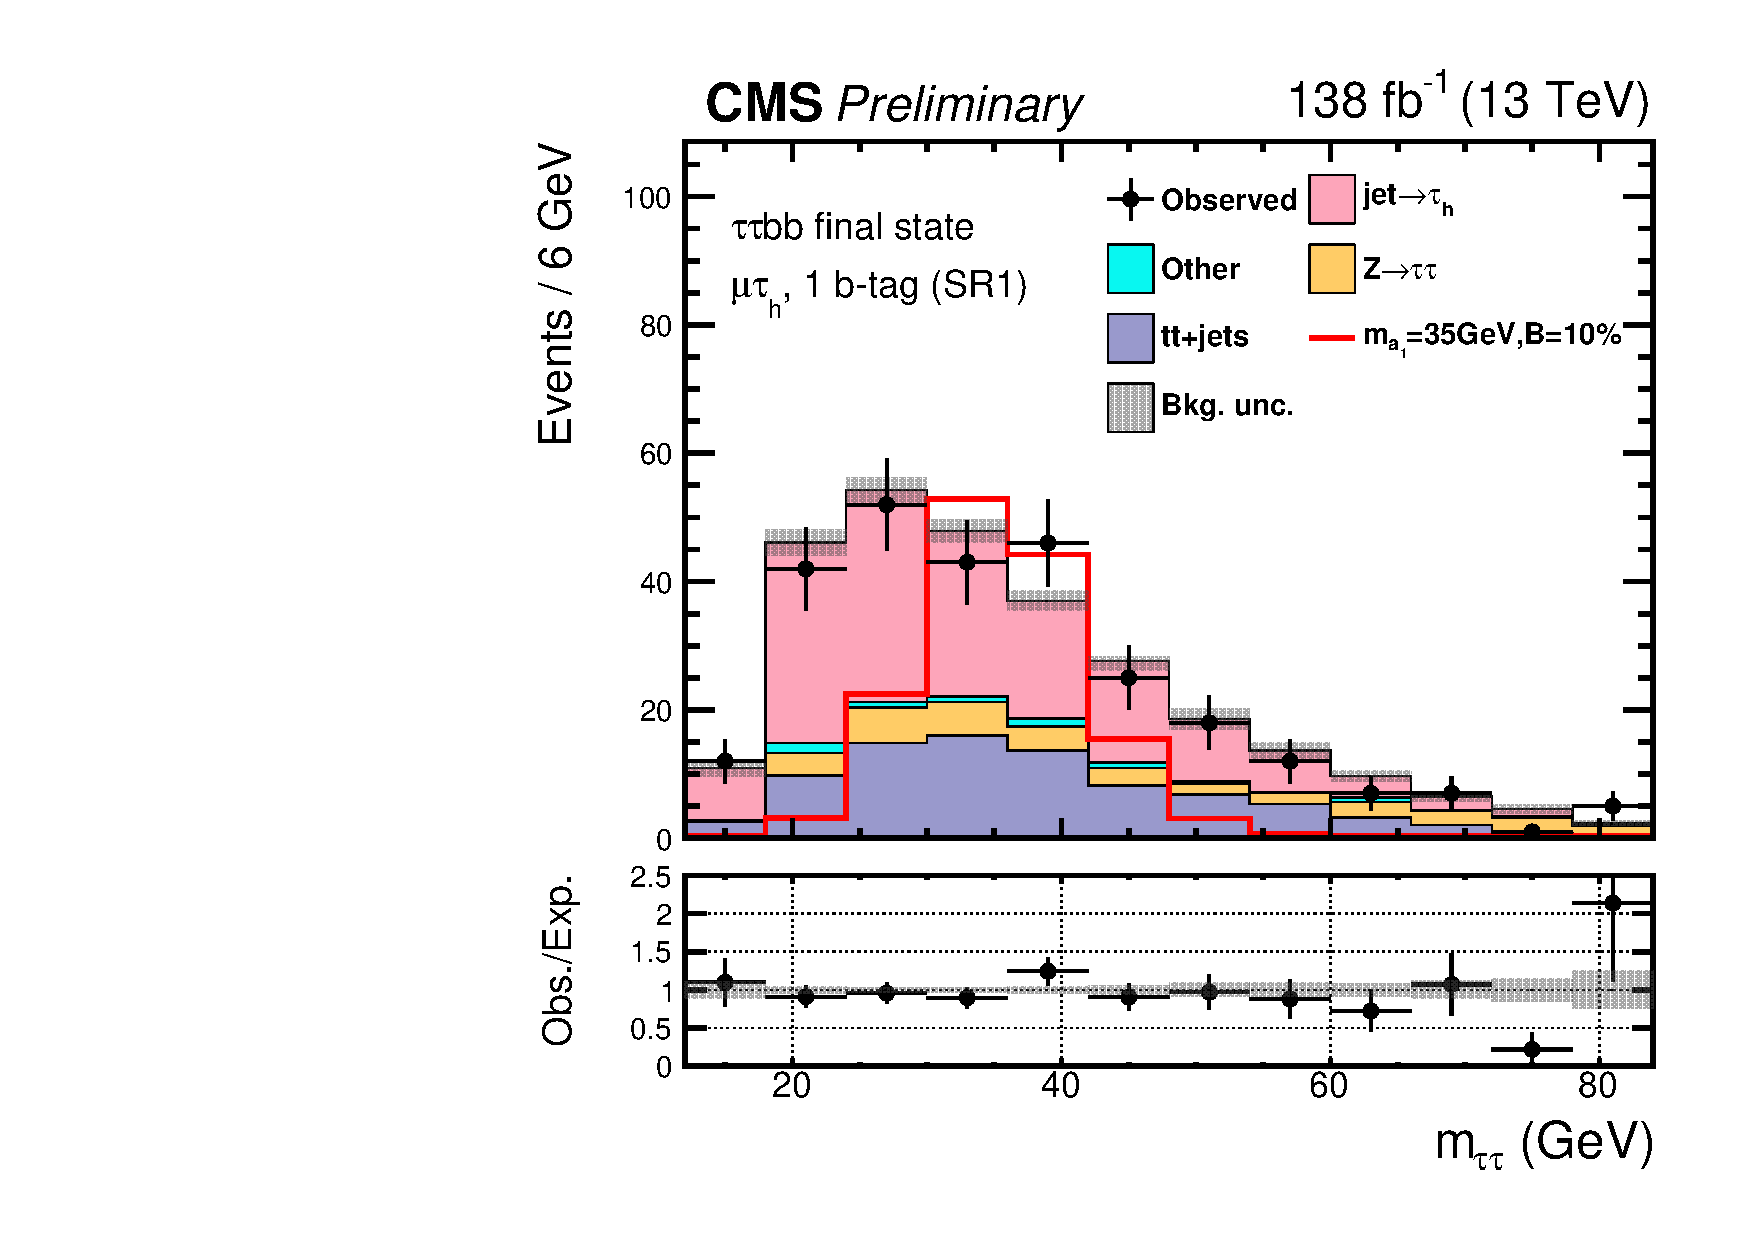
\includegraphics[width=0.32\textwidth]{figures/ch-10-results/mt_all_1_post_prelim-yes.pdf}
        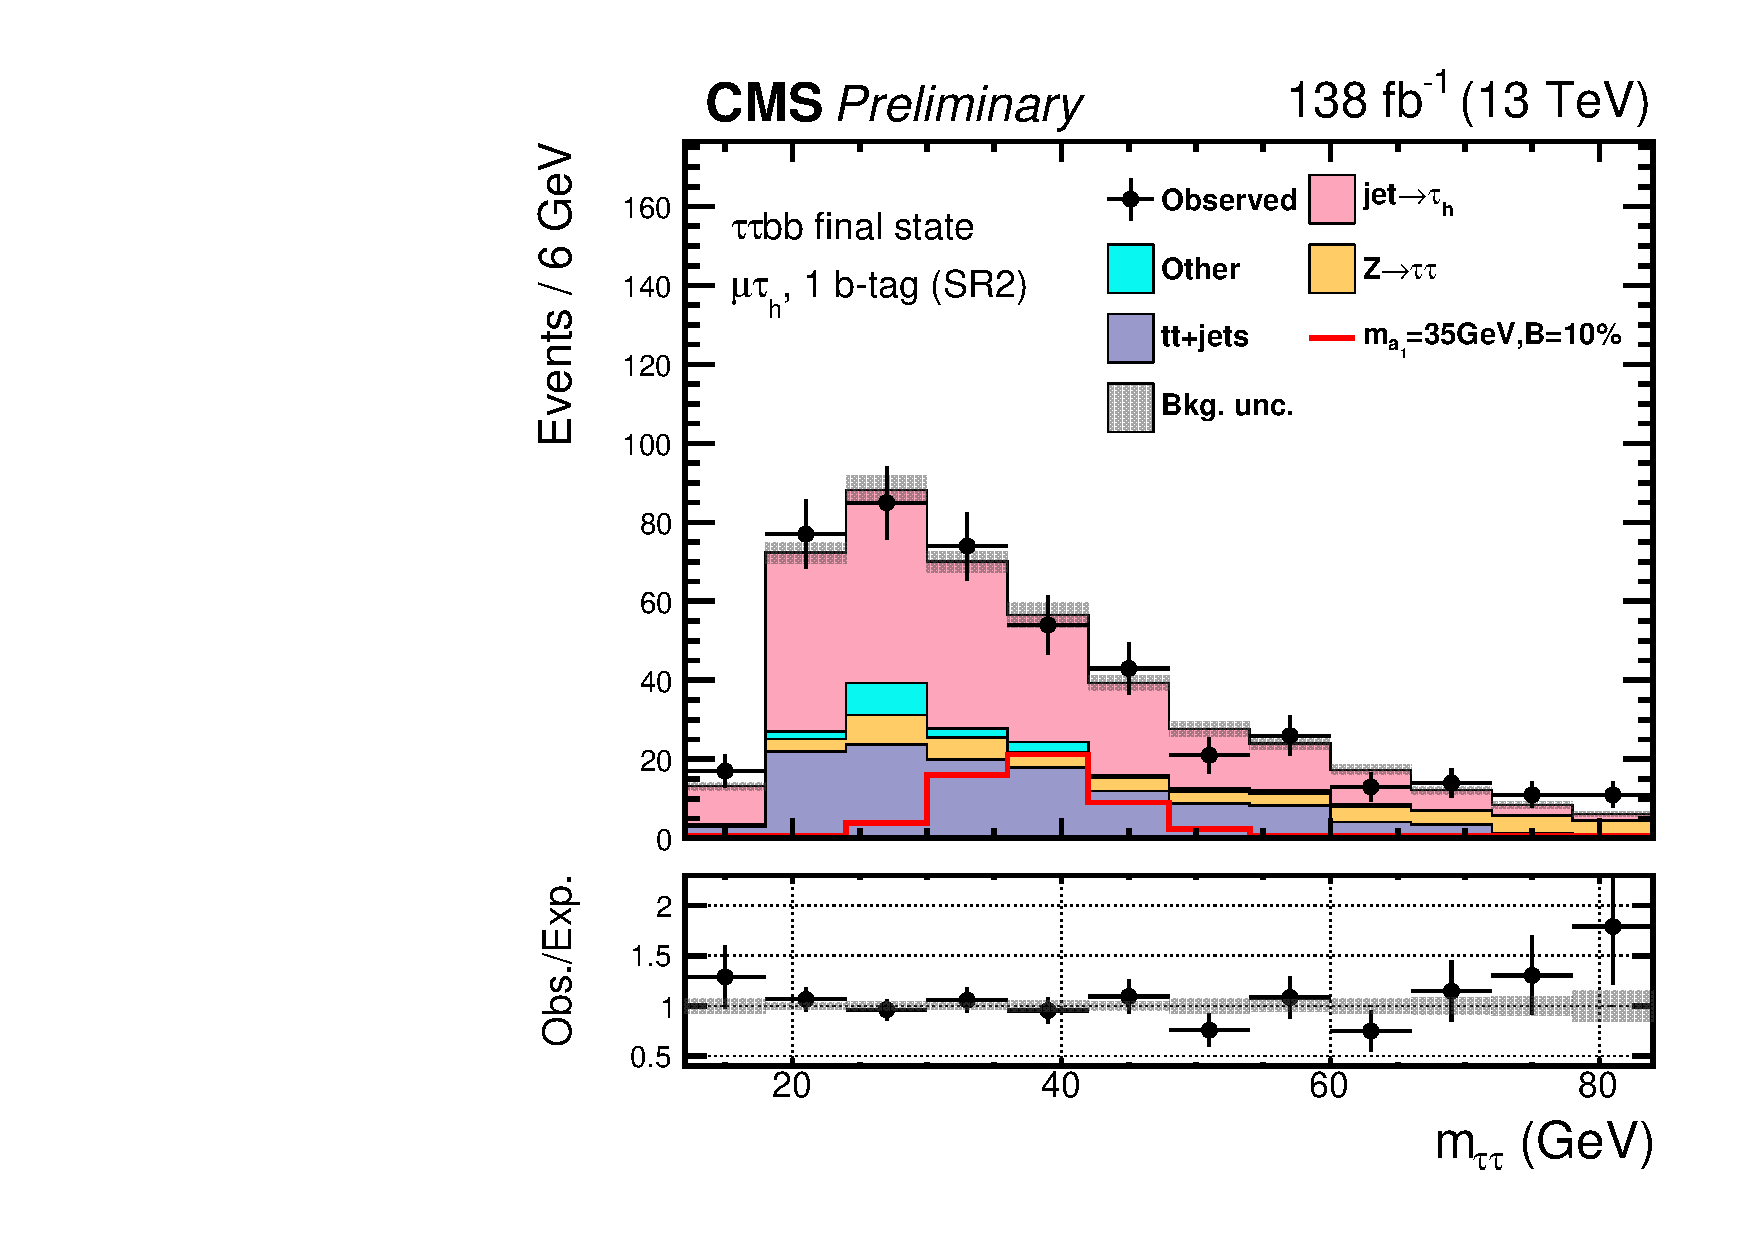
\includegraphics[width=0.32\textwidth]{figures/ch-10-results/mt_all_2_post_prelim-yes.pdf}
        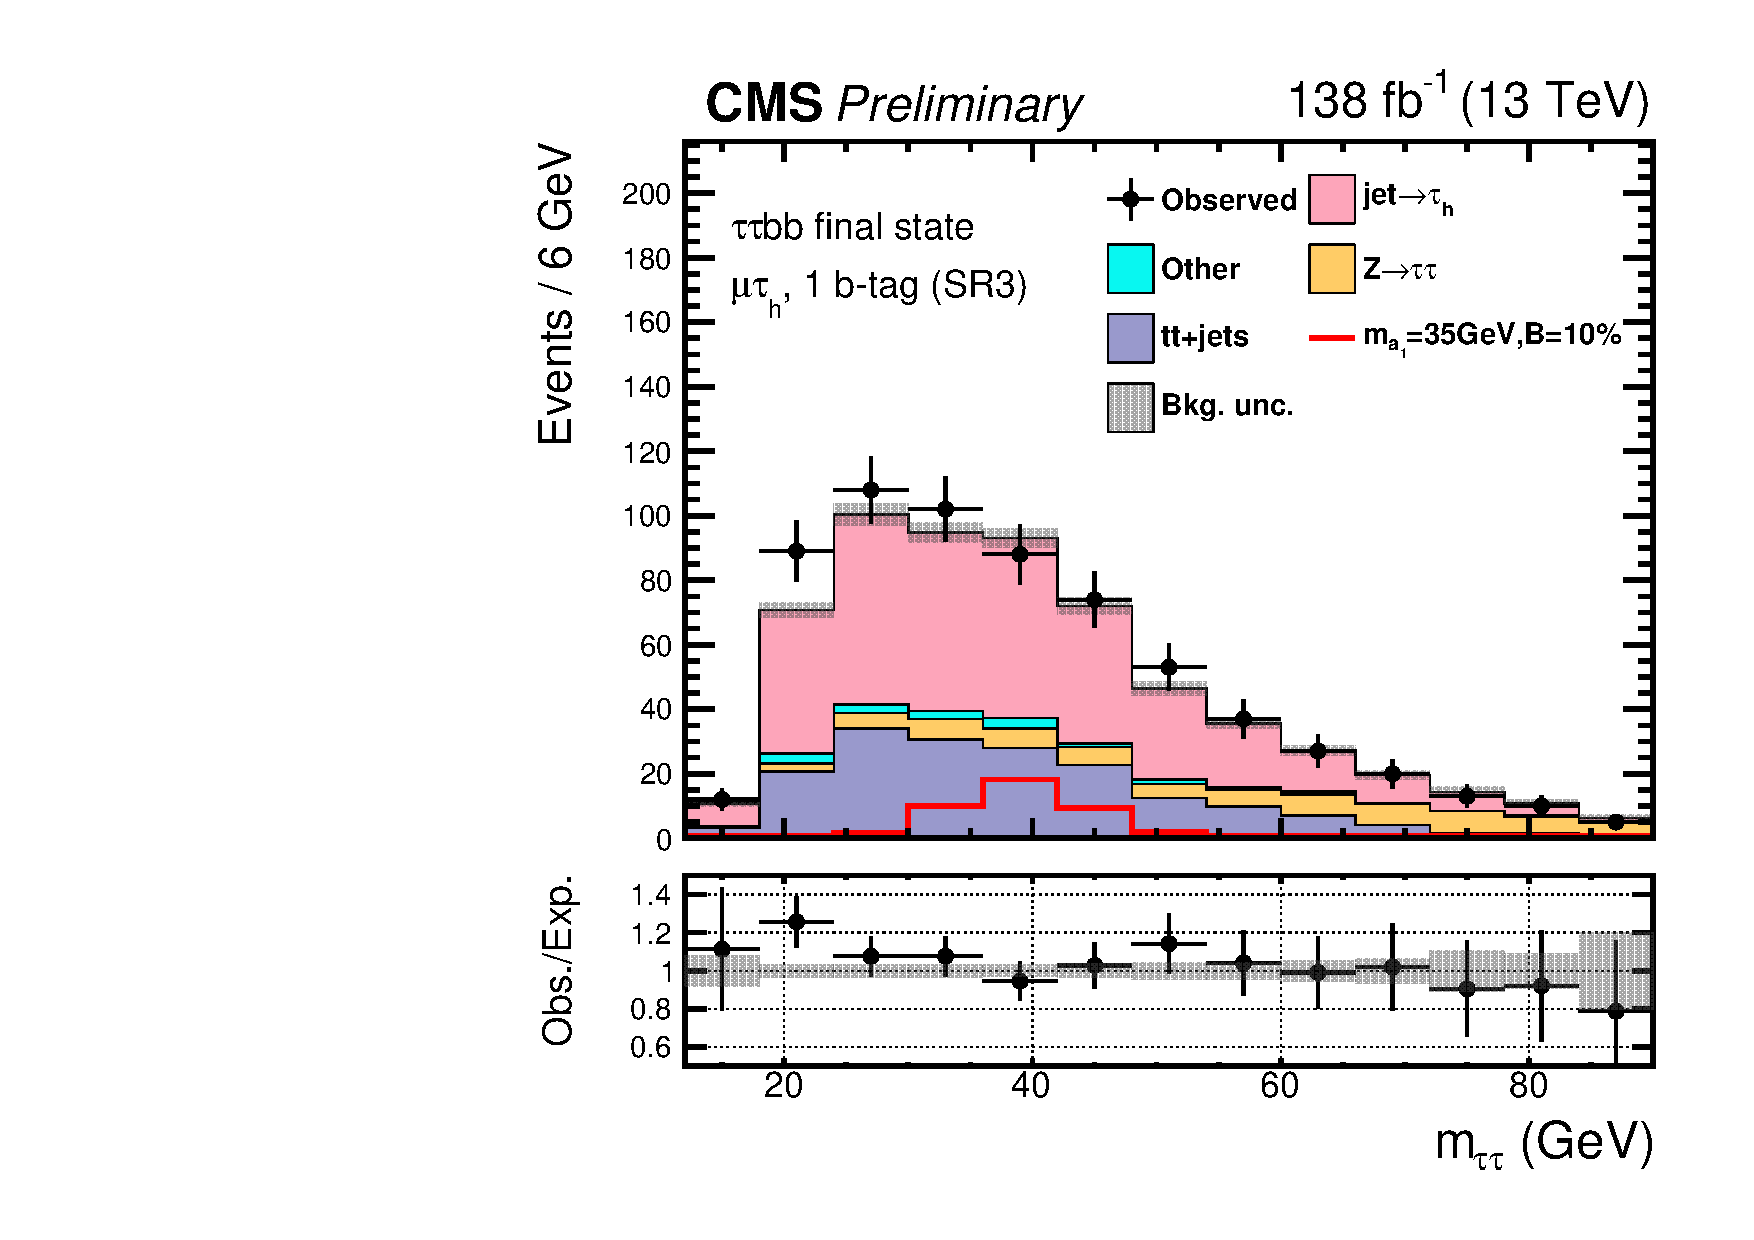
\includegraphics[width=0.32\textwidth]{figures/ch-10-results/mt_all_3_post_prelim-yes.pdf}\\
        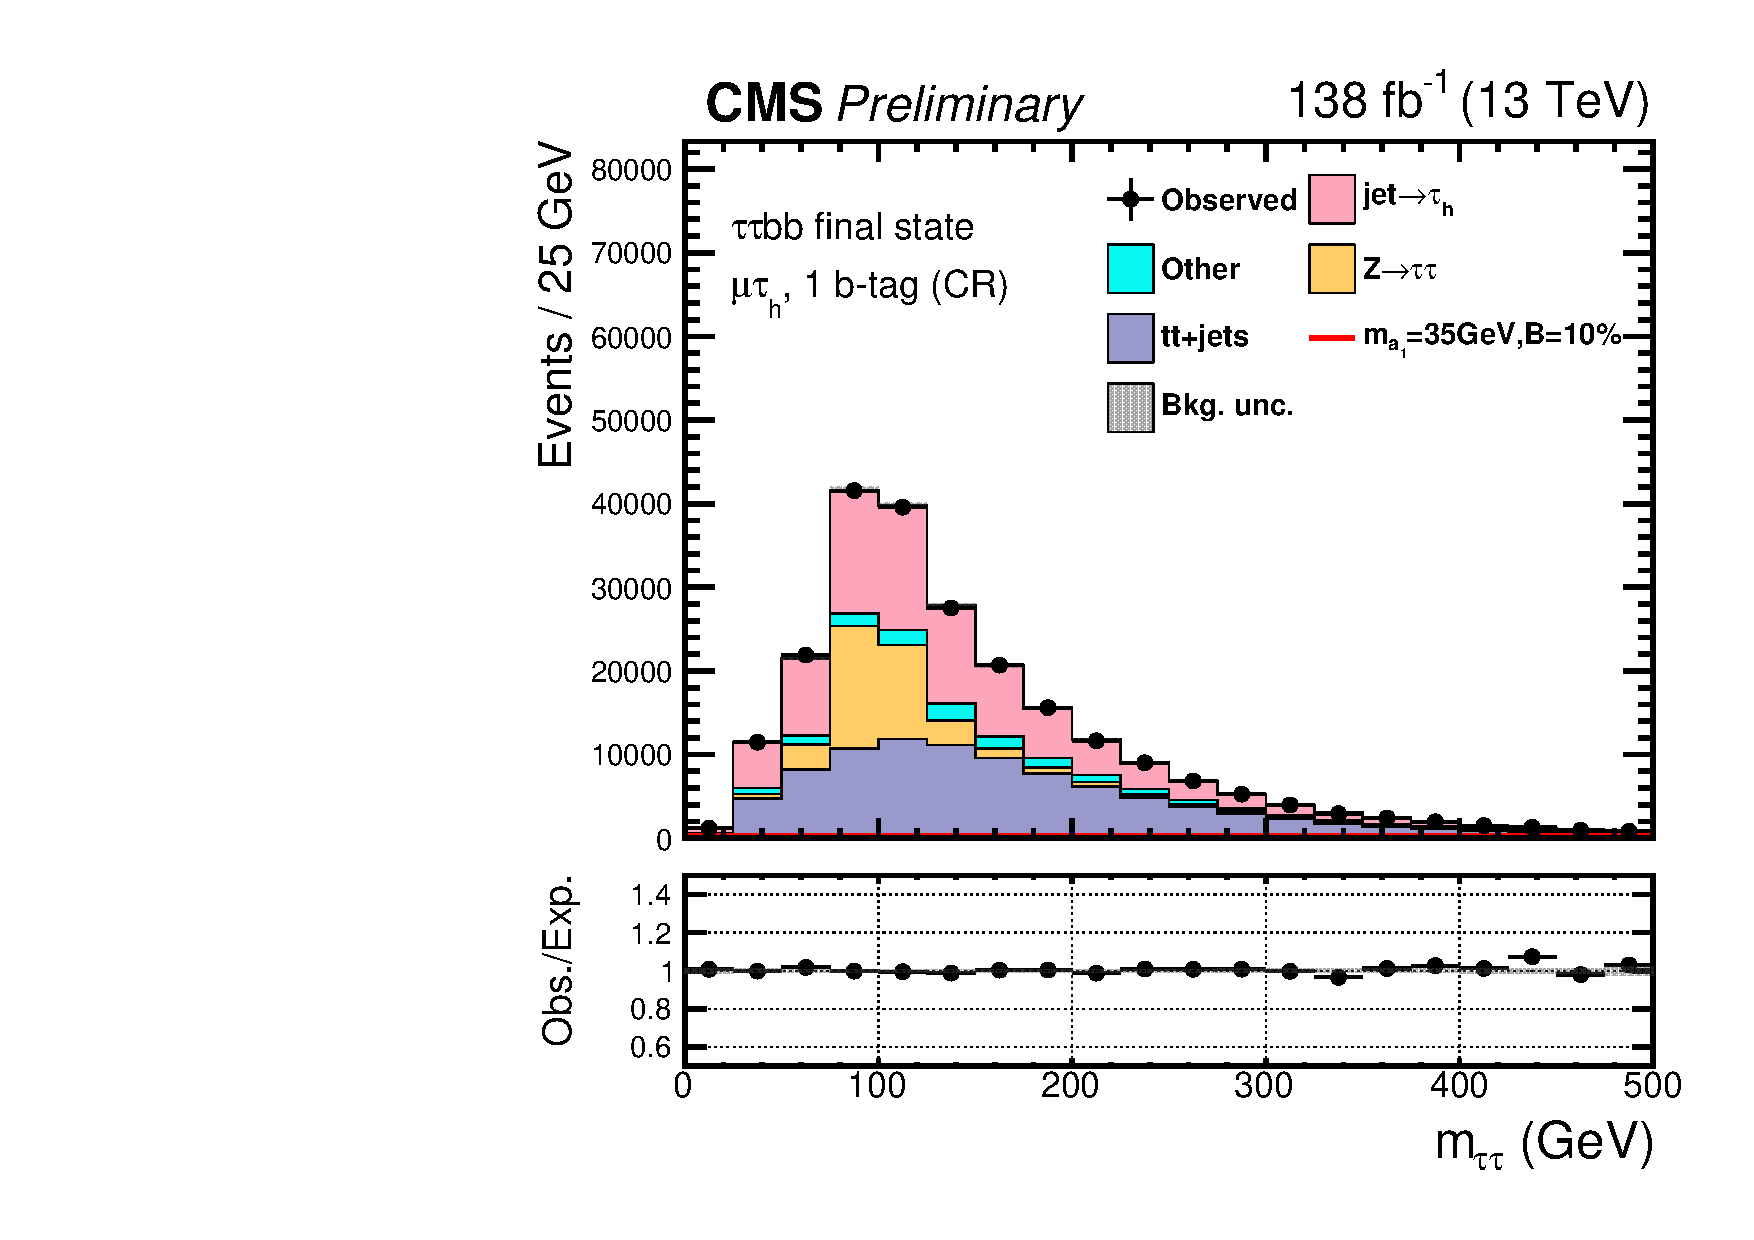
\includegraphics[width=0.32\textwidth]{figures/ch-10-results/mt_all_4_post_prelim-yes.pdf}
        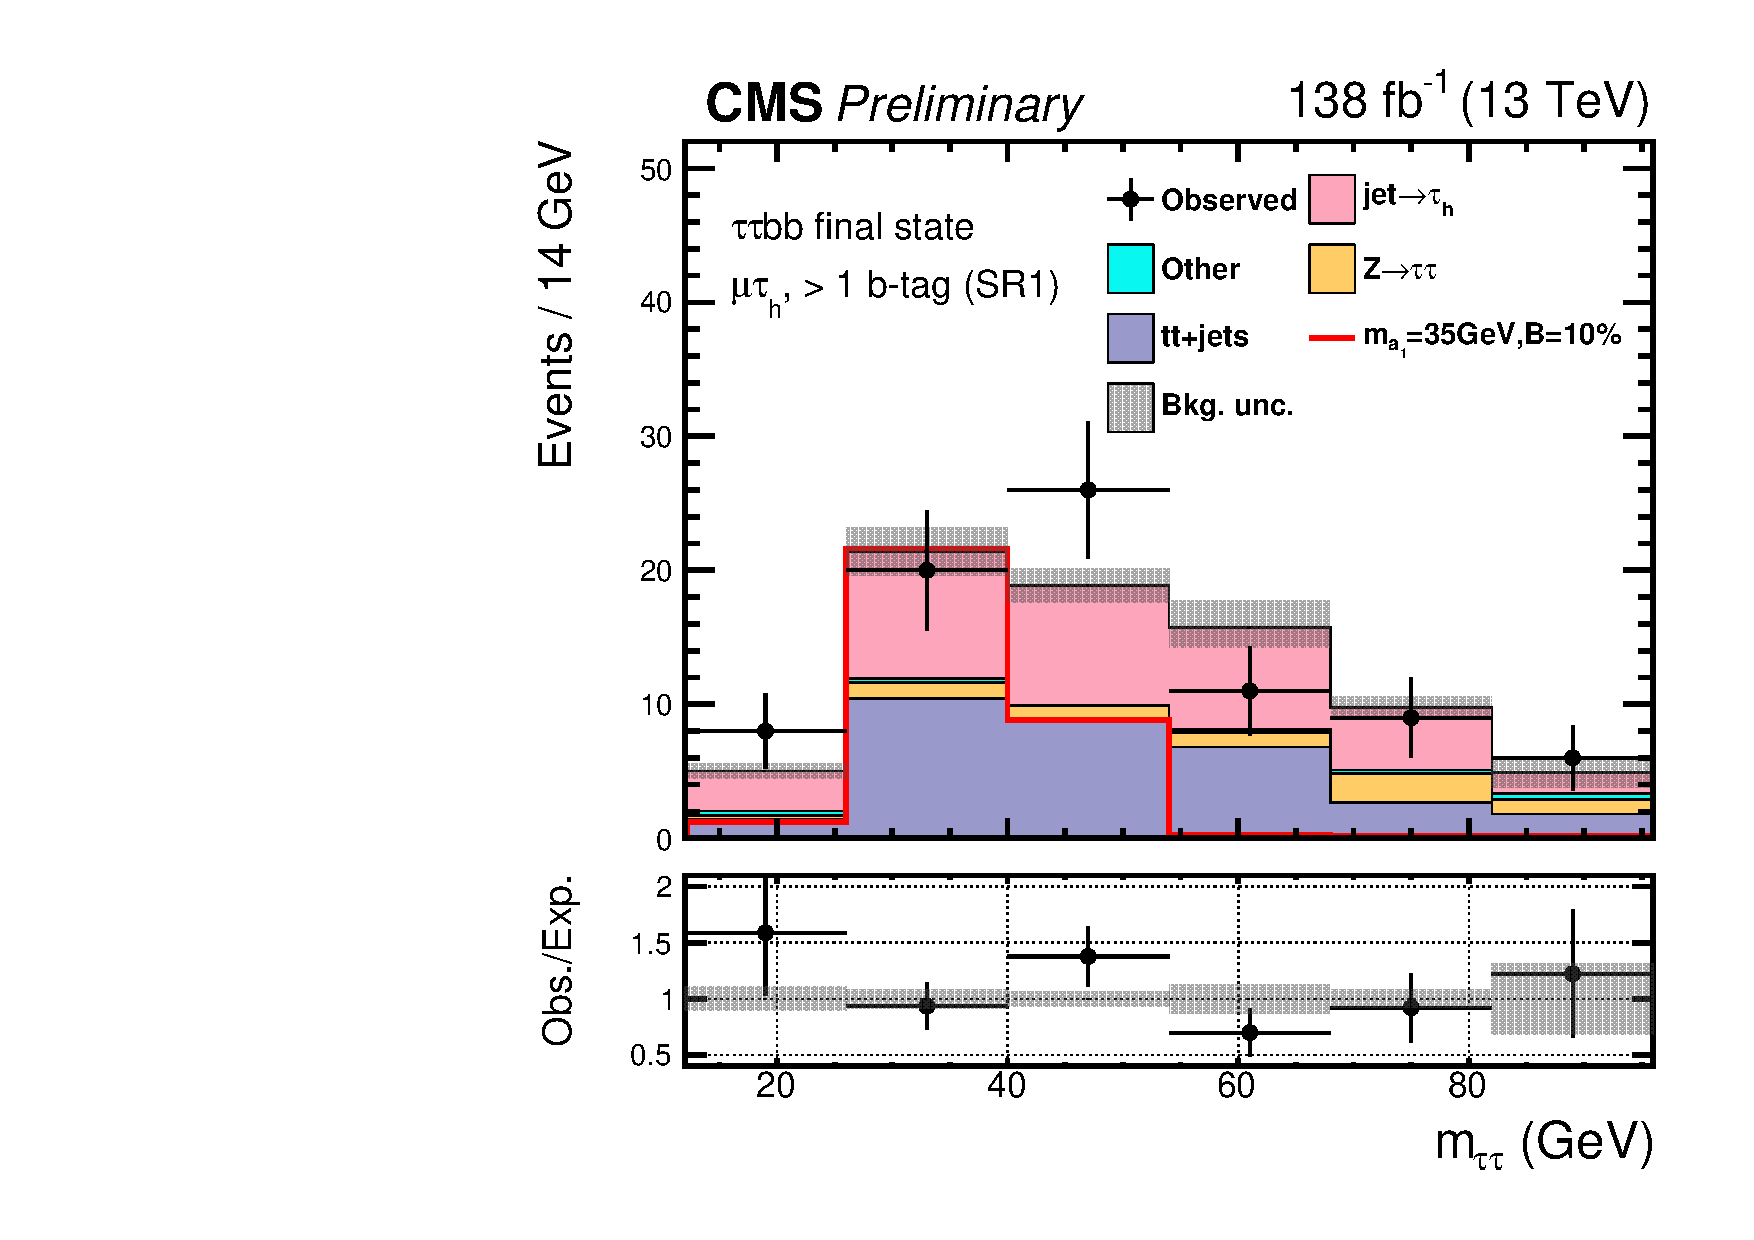
\includegraphics[width=0.32\textwidth]{figures/ch-10-results/mt_all_5_post_prelim-yes.pdf}
        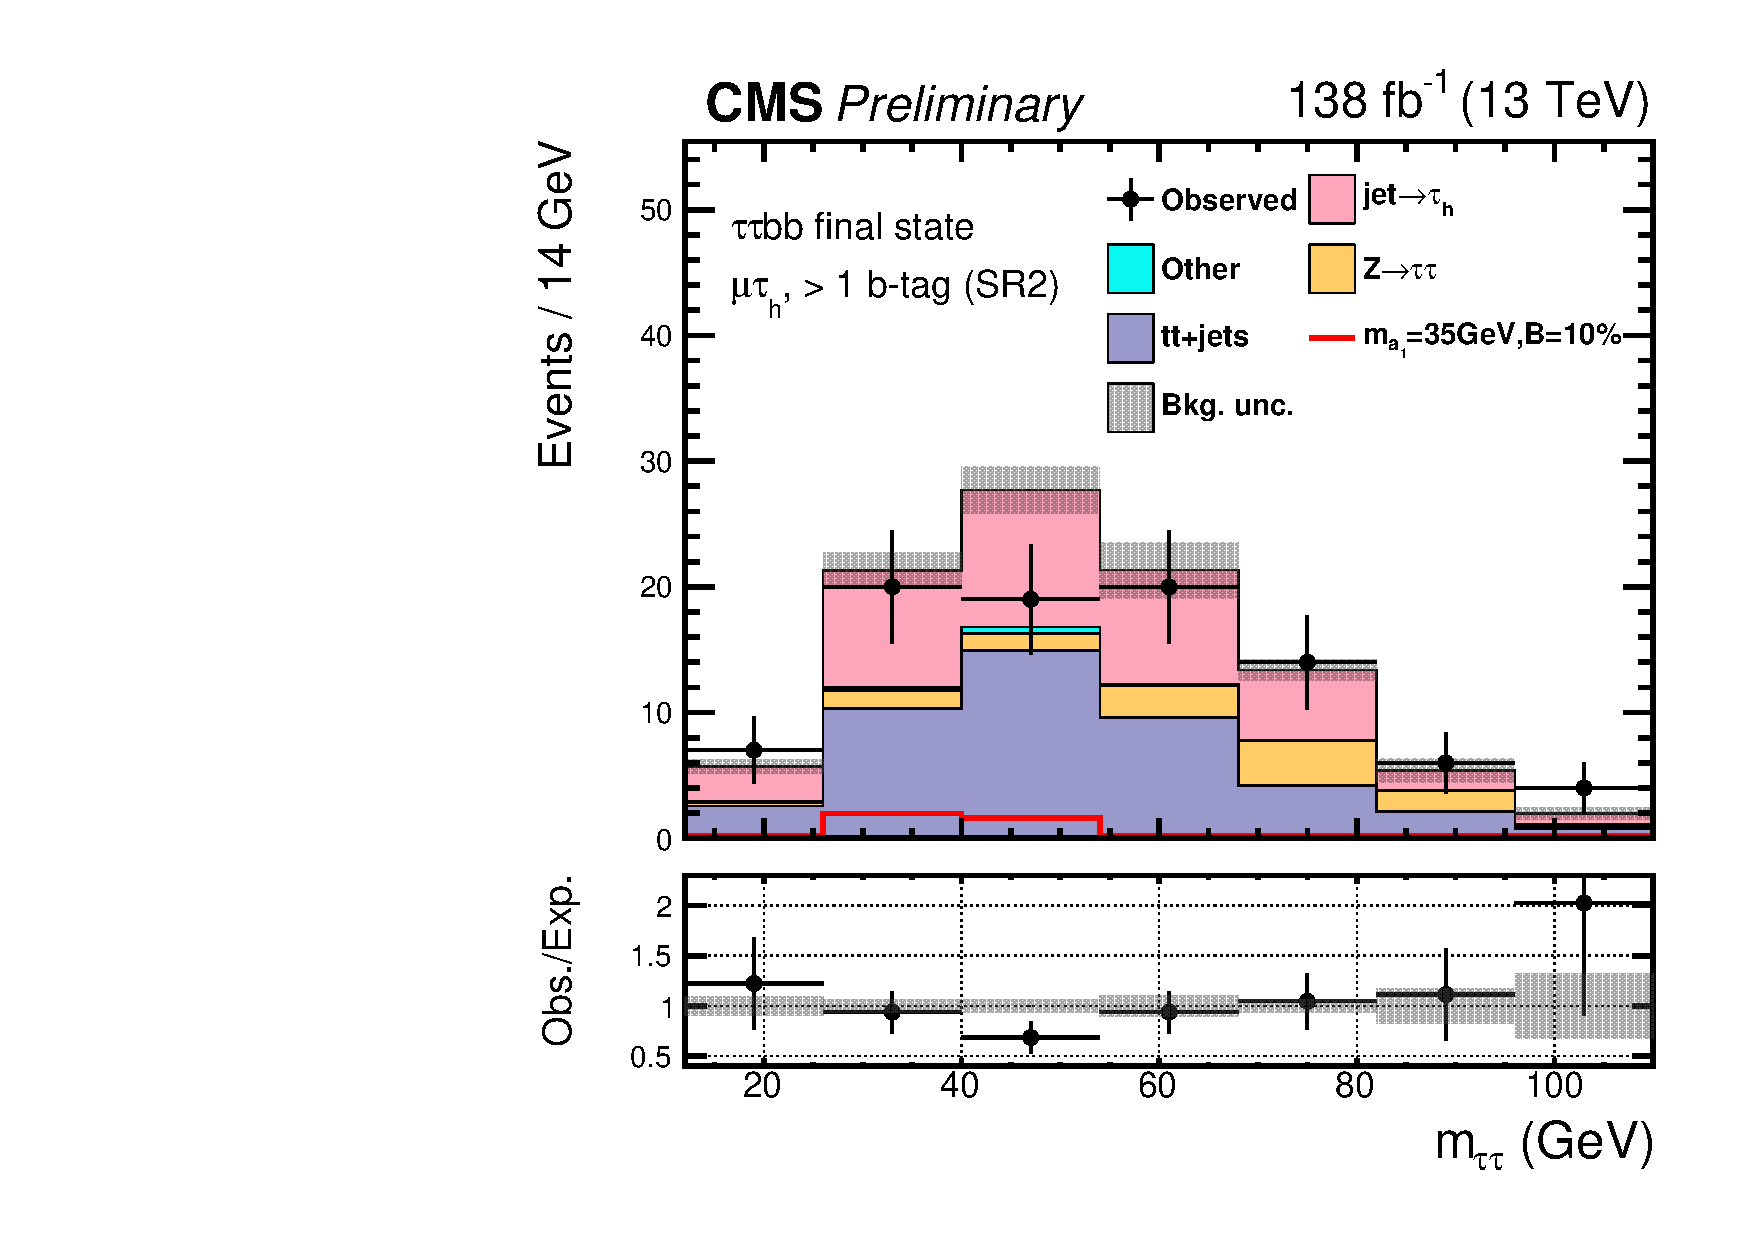
\includegraphics[width=0.32\textwidth]{figures/ch-10-results/mt_all_6_post_prelim-yes.pdf}\\
        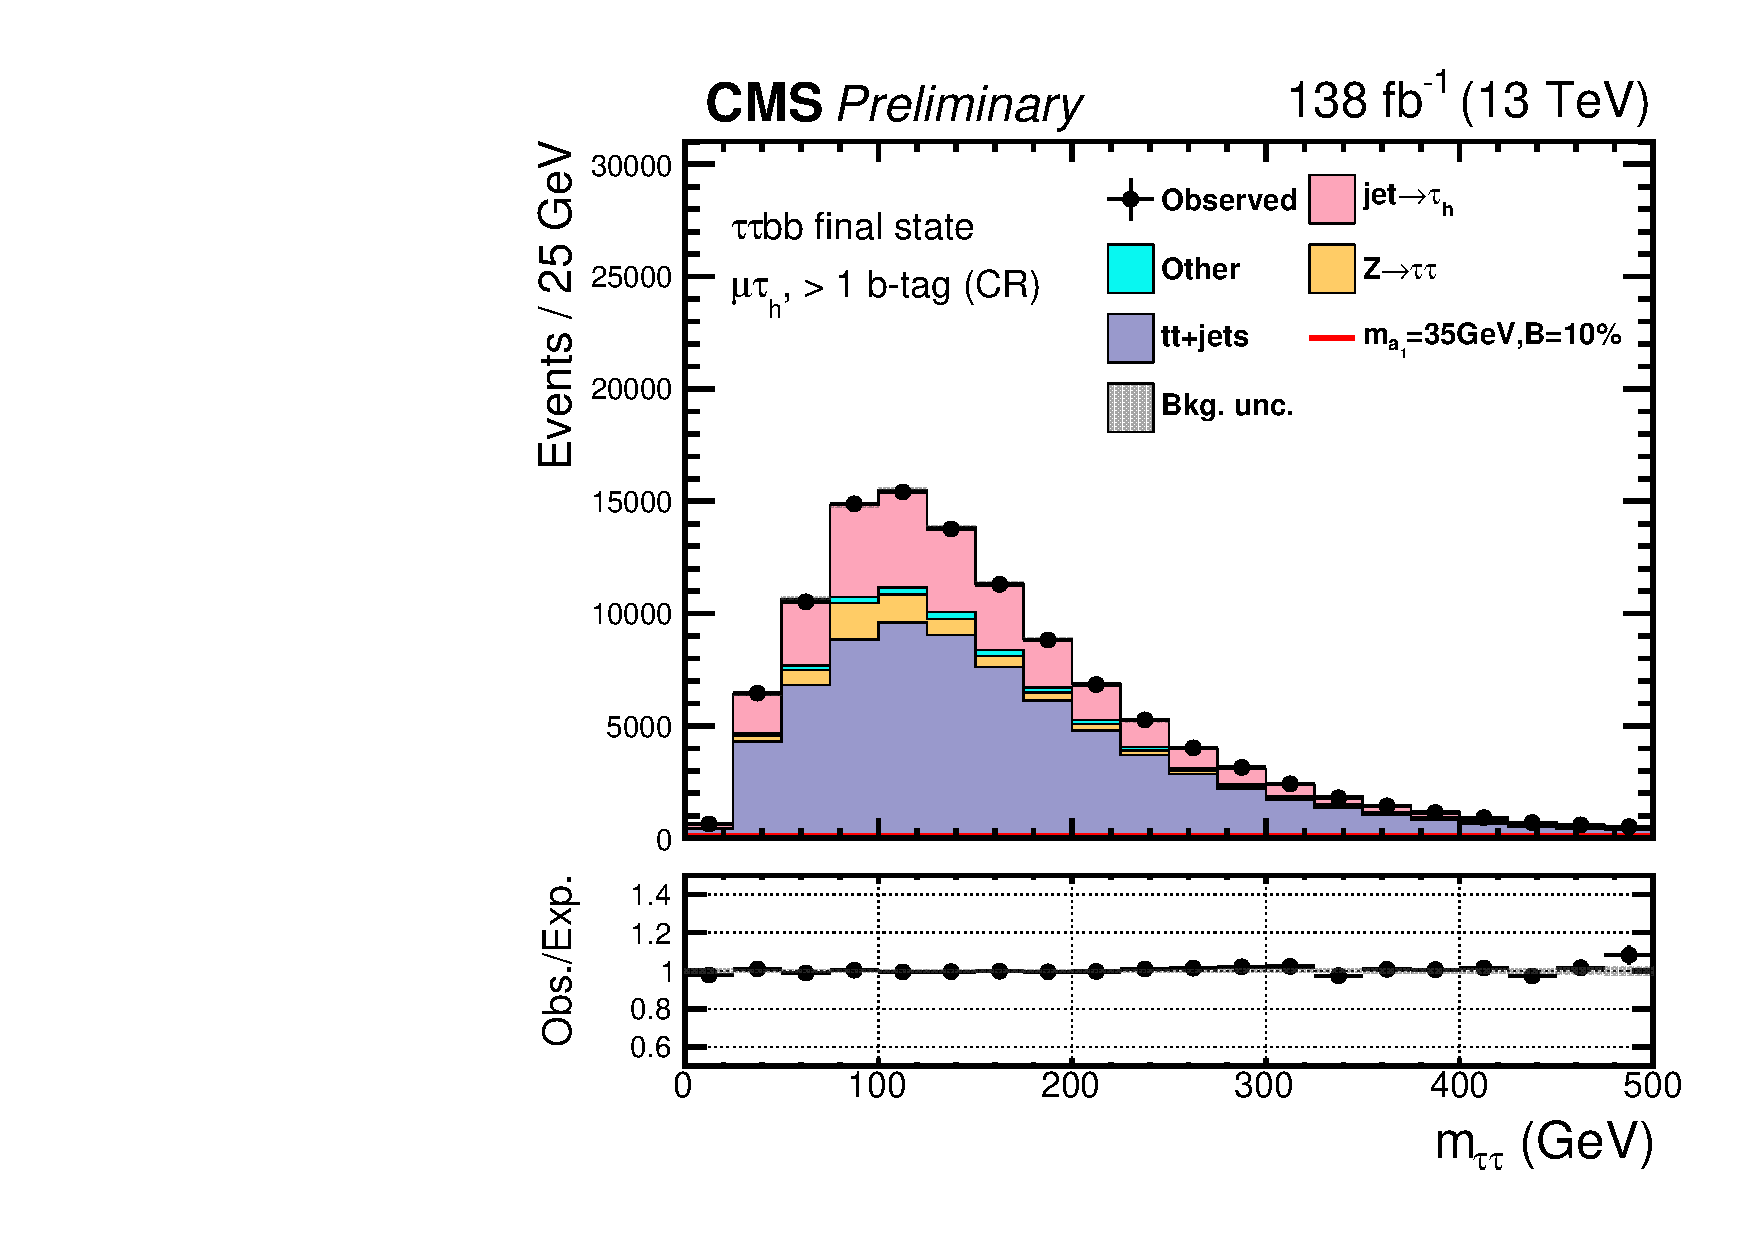
\includegraphics[width=0.32\textwidth]{figures/ch-10-results/mt_all_7_post_prelim-yes.pdf}
    \end{center}
    \caption[Postfit final observed and expected $m_{\tau\tau}$ distributions in the $\mu\tau_{h}$ channel, for the 1 b-tag jet and 2 b-tag jet signal and control regions.]{Postfit final $m_{\tau\tau}$ observed and expected distributions, and the observed/expected ratios, in the $\mu\tau_{h}$ channel \cite{CMS-AN-20-213}. Events are divided into the 1 b-tag jet signal regions (SR1, SR2, SR3) (\textit{top row}), 1 b-tag jet control region (\textit{middle row}), 2 b-tag jet signal regions (SR1, SR2) (\textit{middle row}), and lastly the 2 b-tag jet control region (CR) (\textit{bottom}). Statistical and systematic sources of uncertainties in the expected events are added in quadrature and labeled ``Bkg. unc" (\textit{shaded gray}). The dominant backgrounds in all categories are jets faking the $\tau_{h}$ leg (\textit{pink}), $Z \rightarrow \tau\tau$ (\textit{orange}), and $t\bar{t}$+jets (\textit{purple}). For illustrative purposes, the beyond-Standard Model signal yield from $h\rightarrow aa bb\tau\tau$ is shown for the pseudoscalar mass hypothesis $m_a = 35$ GeV, assuming a branching fraction $B(h \rightarrow aa \rightarrow bb\tau\tau) = 10\%$ (\textit{red line}).}
    \label{fig:results_mtt_postfit_mtall}
\end{figure}

\begin{figure}[ht]
    \begin{center}
        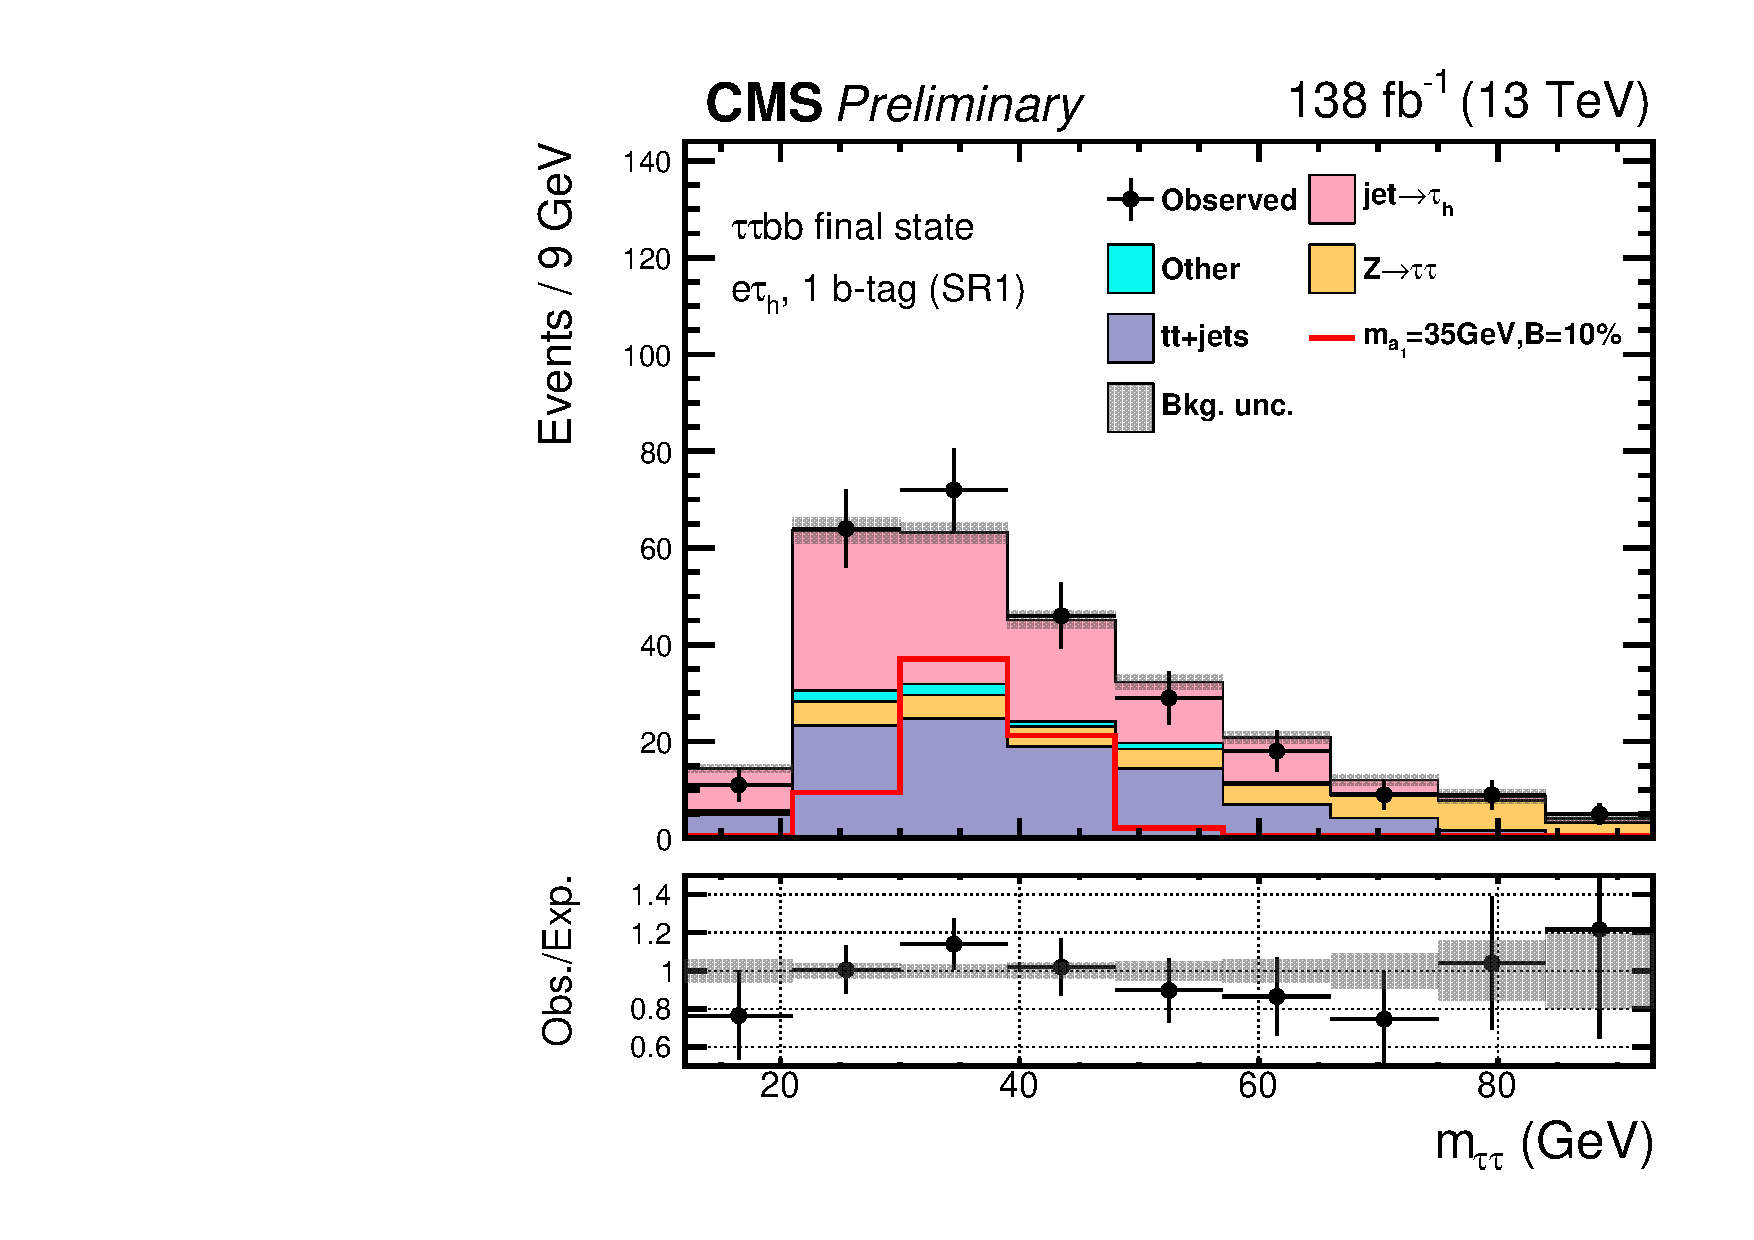
\includegraphics[width=0.32\textwidth]{figures/ch-10-results/et_all_1_post_prelim-yes.pdf}
        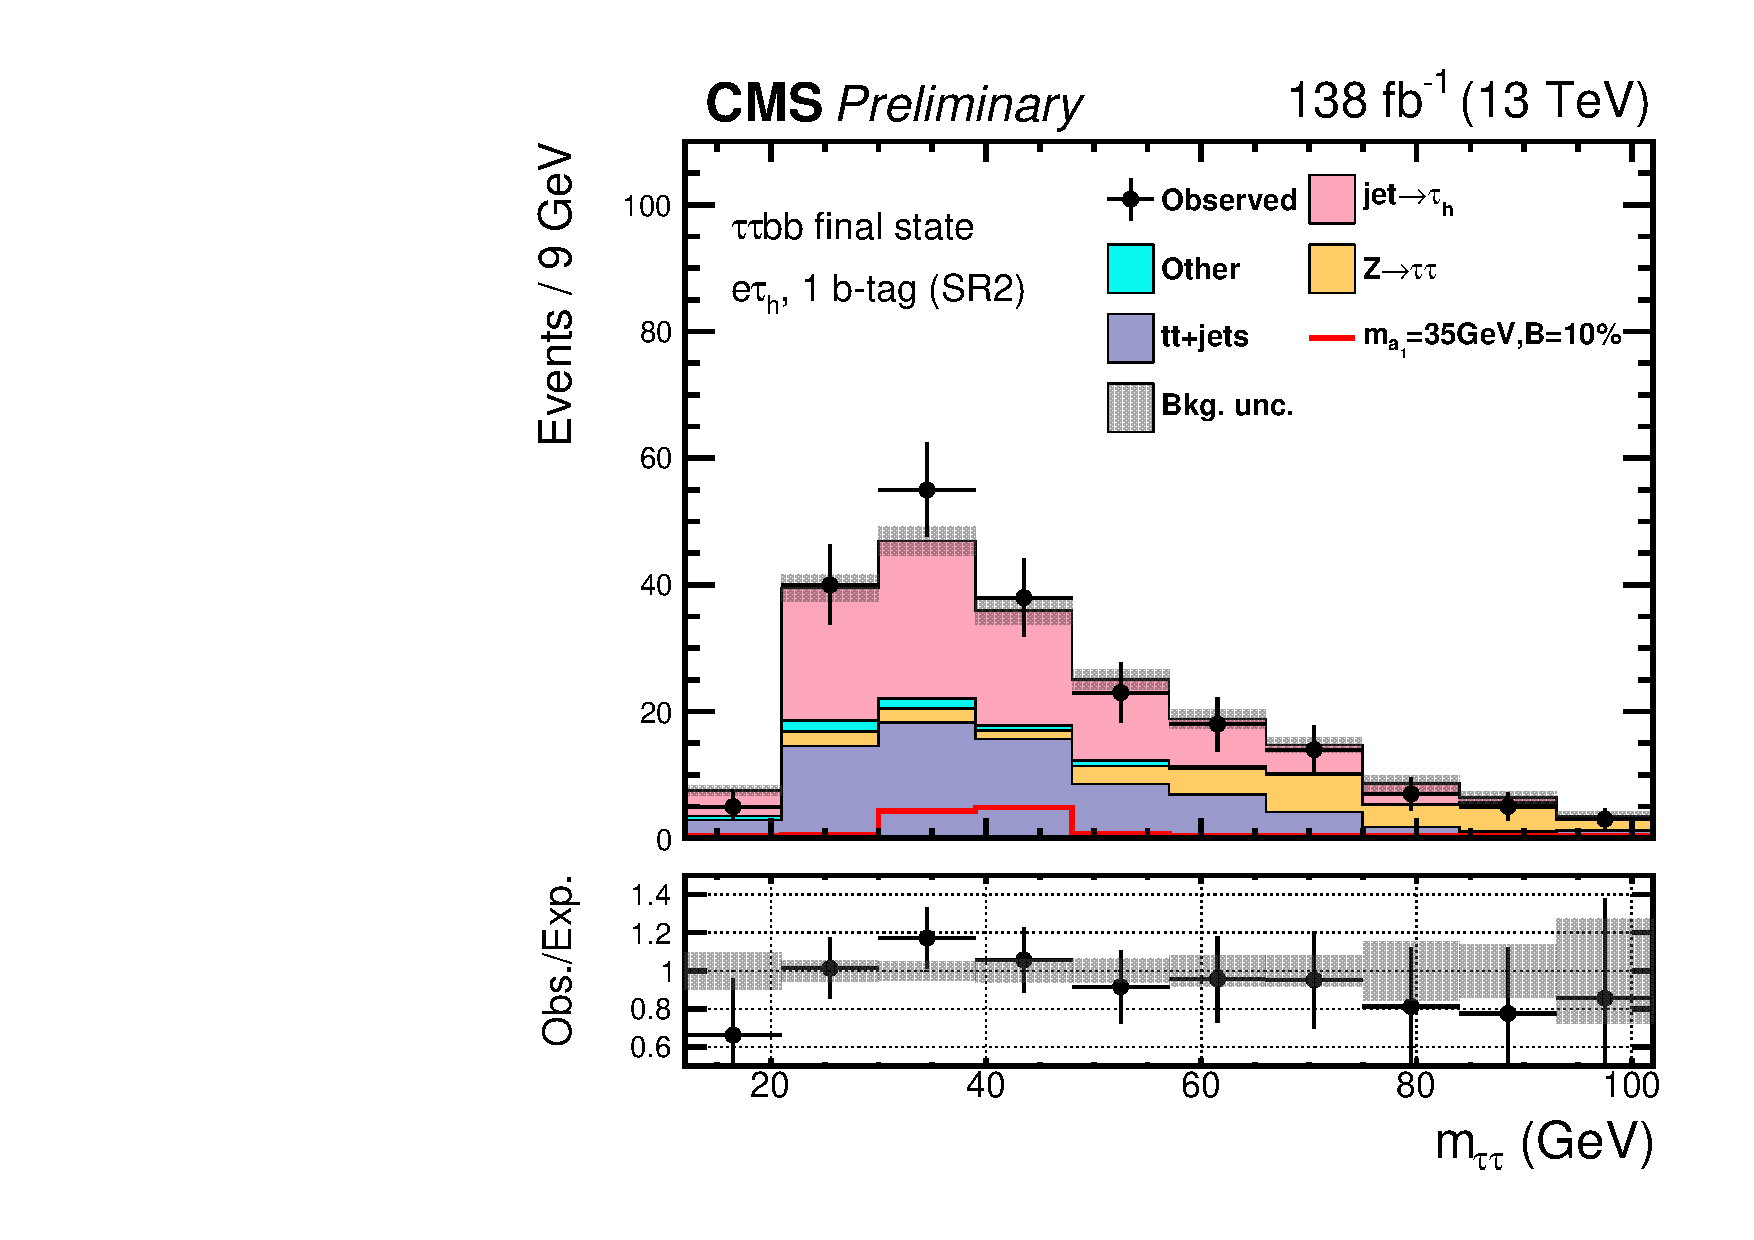
\includegraphics[width=0.32\textwidth]{figures/ch-10-results/et_all_2_post_prelim-yes.pdf}
        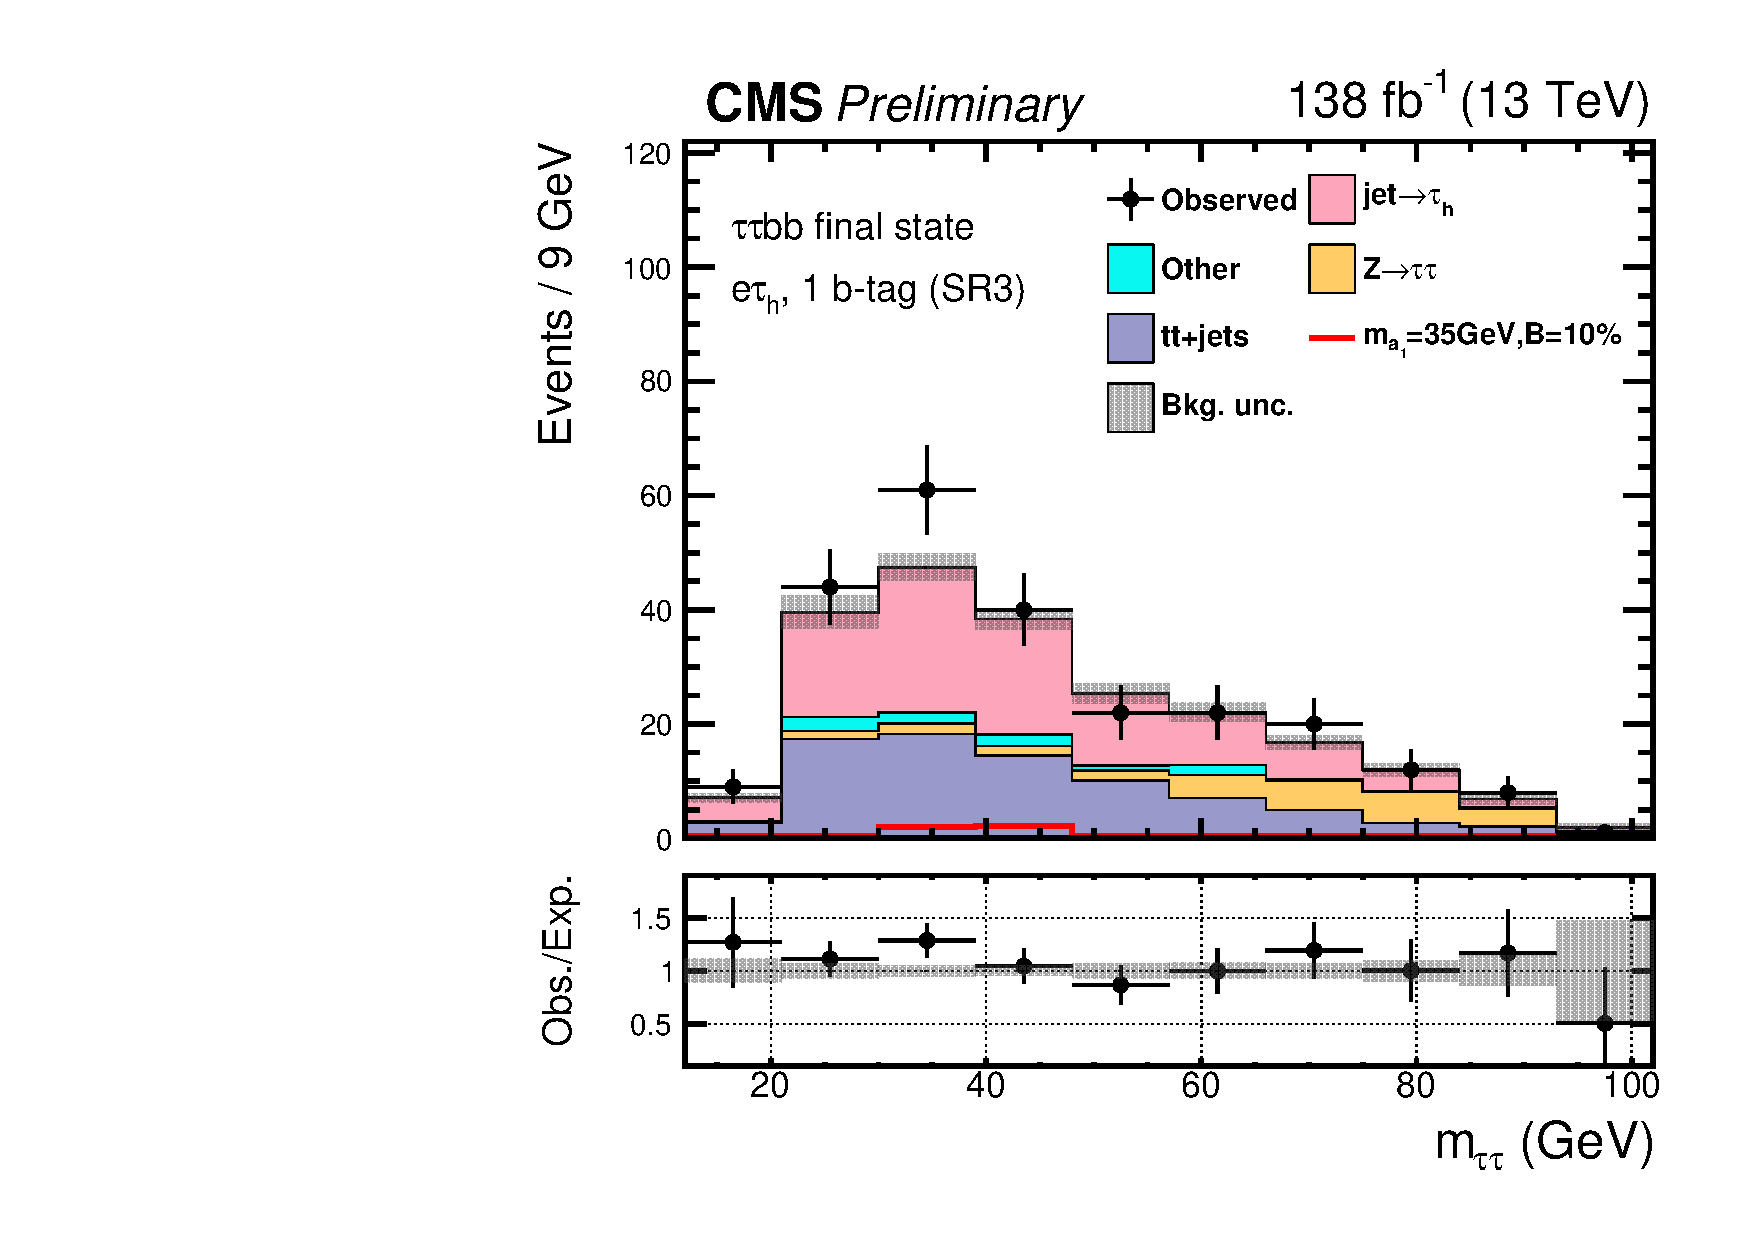
\includegraphics[width=0.32\textwidth]{figures/ch-10-results/et_all_3_post_prelim-yes.pdf}\\
        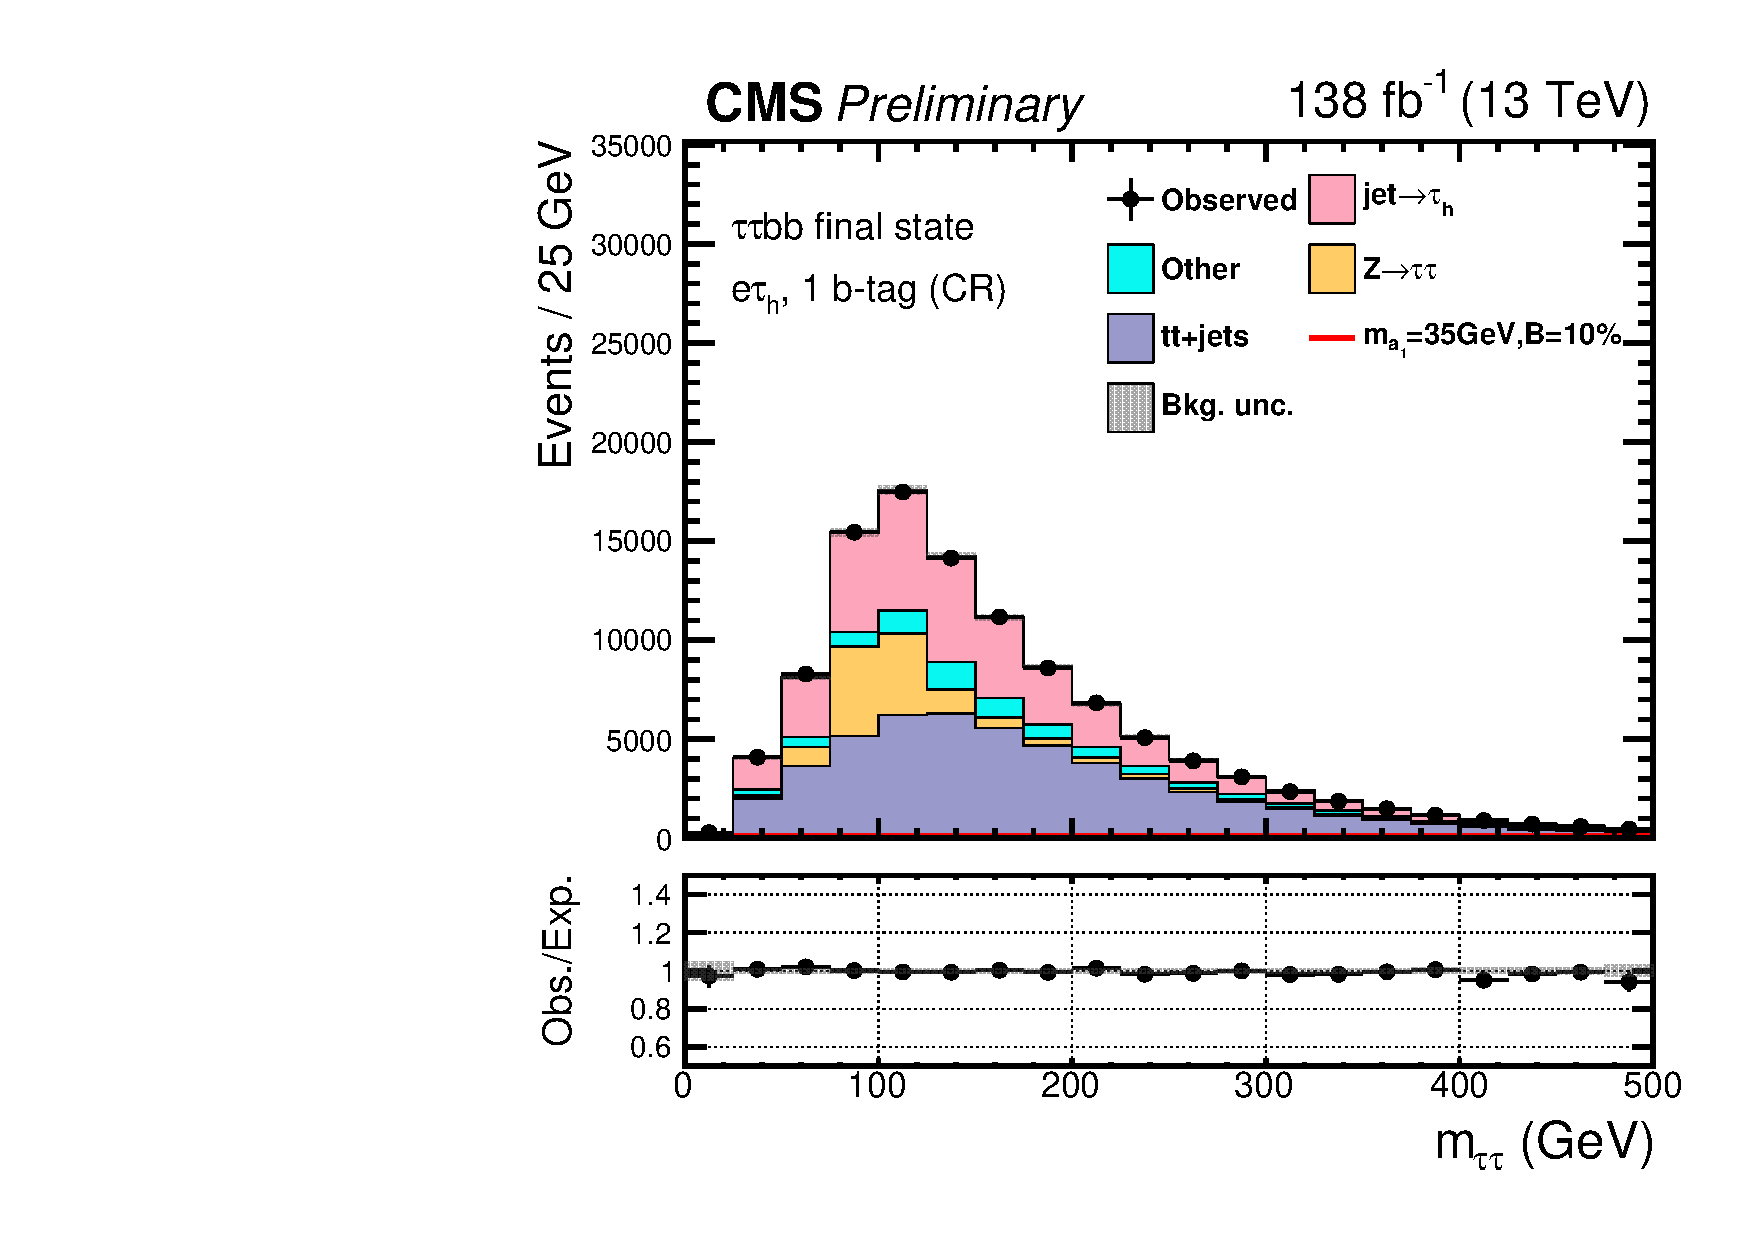
\includegraphics[width=0.32\textwidth]{figures/ch-10-results/et_all_4_post_prelim-yes.pdf}
        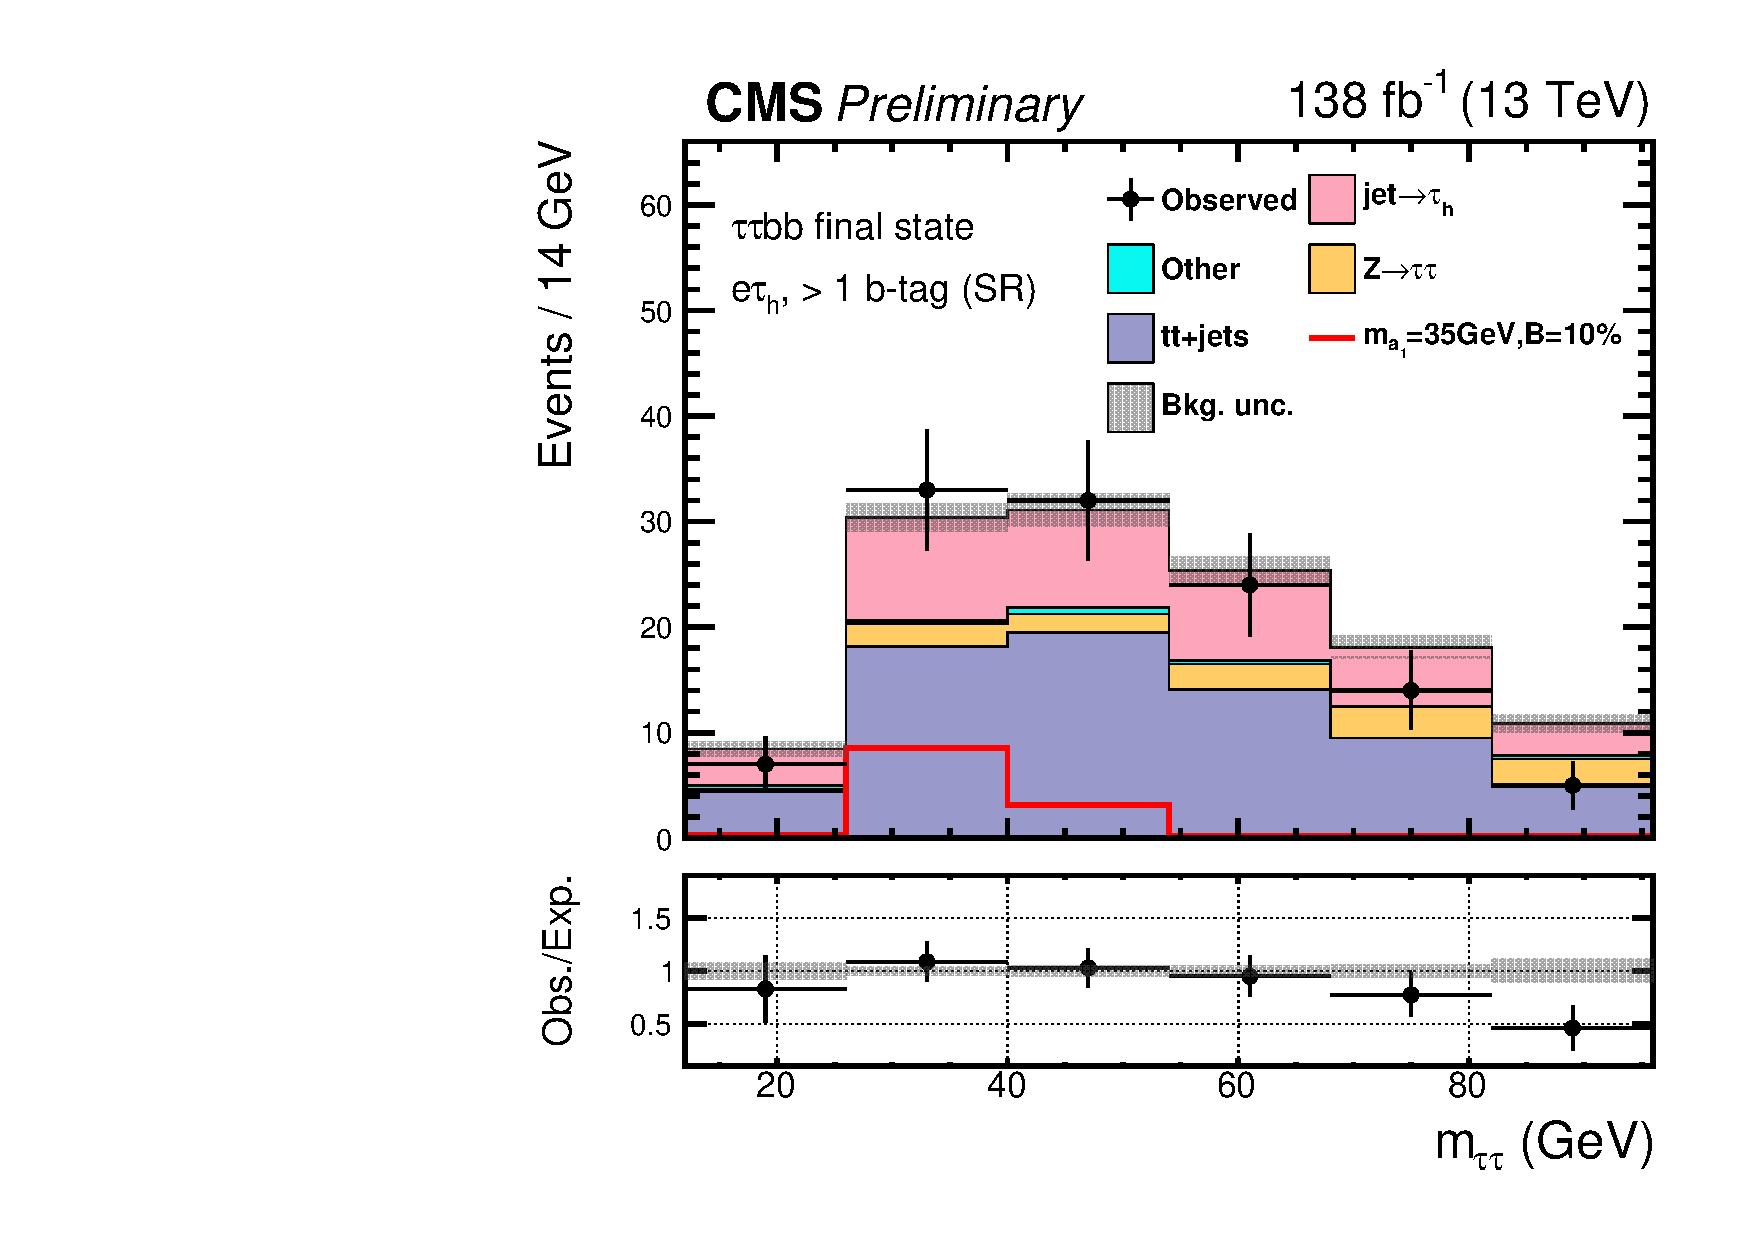
\includegraphics[width=0.32\textwidth]{figures/ch-10-results/et_all_5_post_prelim-yes.pdf}
        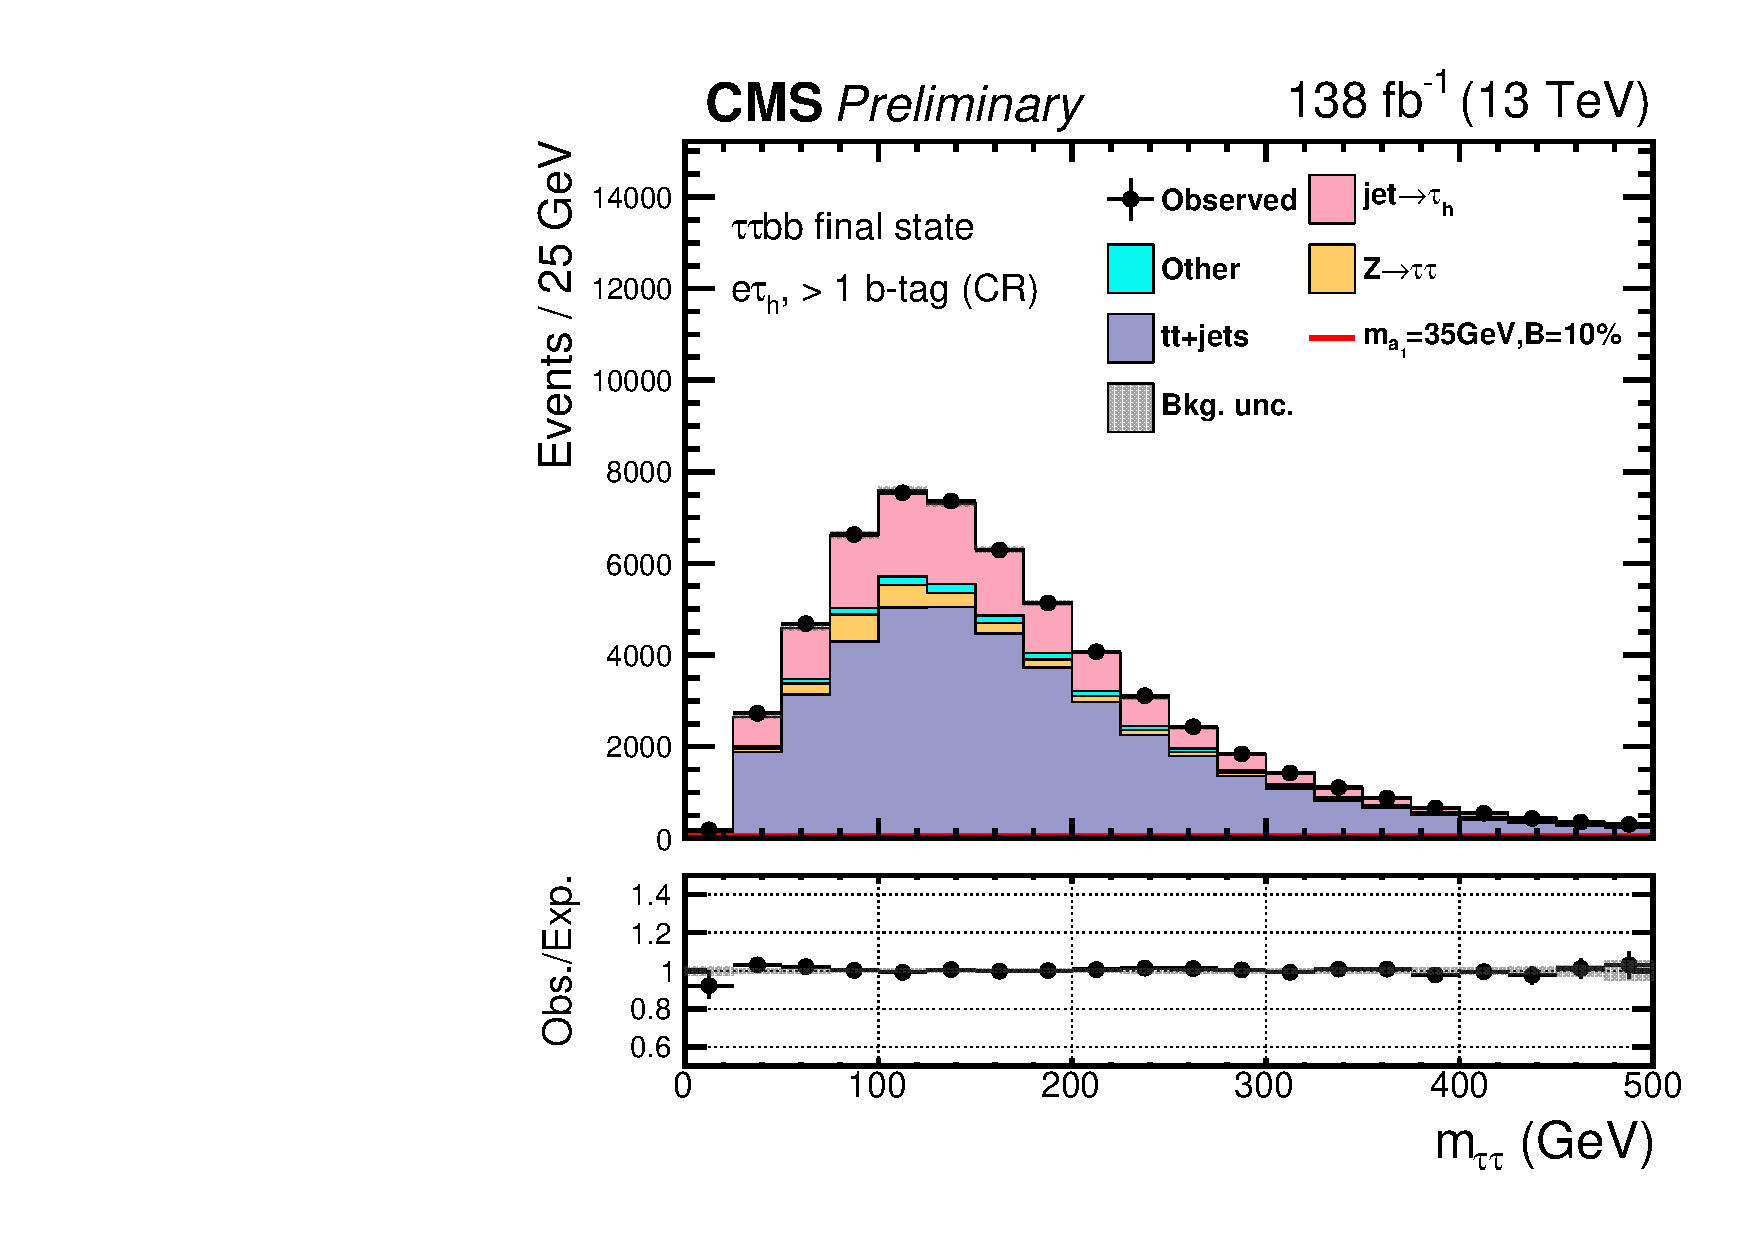
\includegraphics[width=0.32\textwidth]{figures/ch-10-results/et_all_6_post_prelim-yes.pdf}
    \end{center}
    \caption[Postfit final observed and expected $m_{\tau\tau}$ distributions in the $e\tau_{h}$ channel, for the 1 b-tag jet and 2 b-tag jet signal and control regions.]{Postfit final observed and expected $m_{\tau\tau}$ distributions, and the observed/expected ratios, in the $e\tau_{h}$ channel \cite{CMS-AN-20-213}. Events are divided into the 1 b-tag jet signal regions (SR1, SR2, SR3) (\textit{top row}), the 1 b-tag jet control region (CR) (\textit{bottom row}), and 2 b-tag jet signal region (SR) and control region (CR) (\textit{bottom row}). Statistical and systematic sources of uncertainties in the expected events are added in quadrature and labeled ``Bkg. unc" (\textit{shaded gray}). In this channel, the dominant backgrounds are jets faking the $\tau_{h}$ leg (\textit{pink}), $Z \rightarrow \tau\tau$ (\textit{orange}), and $t\bar{t}$+jets (\textit{purple}). For illustrative purposes, the beyond-Standard Model signal yield from $h\rightarrow aa bb\tau\tau$ is shown for the pseudoscalar mass hypothesis $m_a = 35$ GeV, assuming a branching fraction $B(h \rightarrow aa \rightarrow bb\tau\tau) = 10\%$ (\textit{red line}).}
    \label{fig:results_mtt_postfit_etall}
\end{figure}

\begin{figure}[ht]
    \begin{center}
        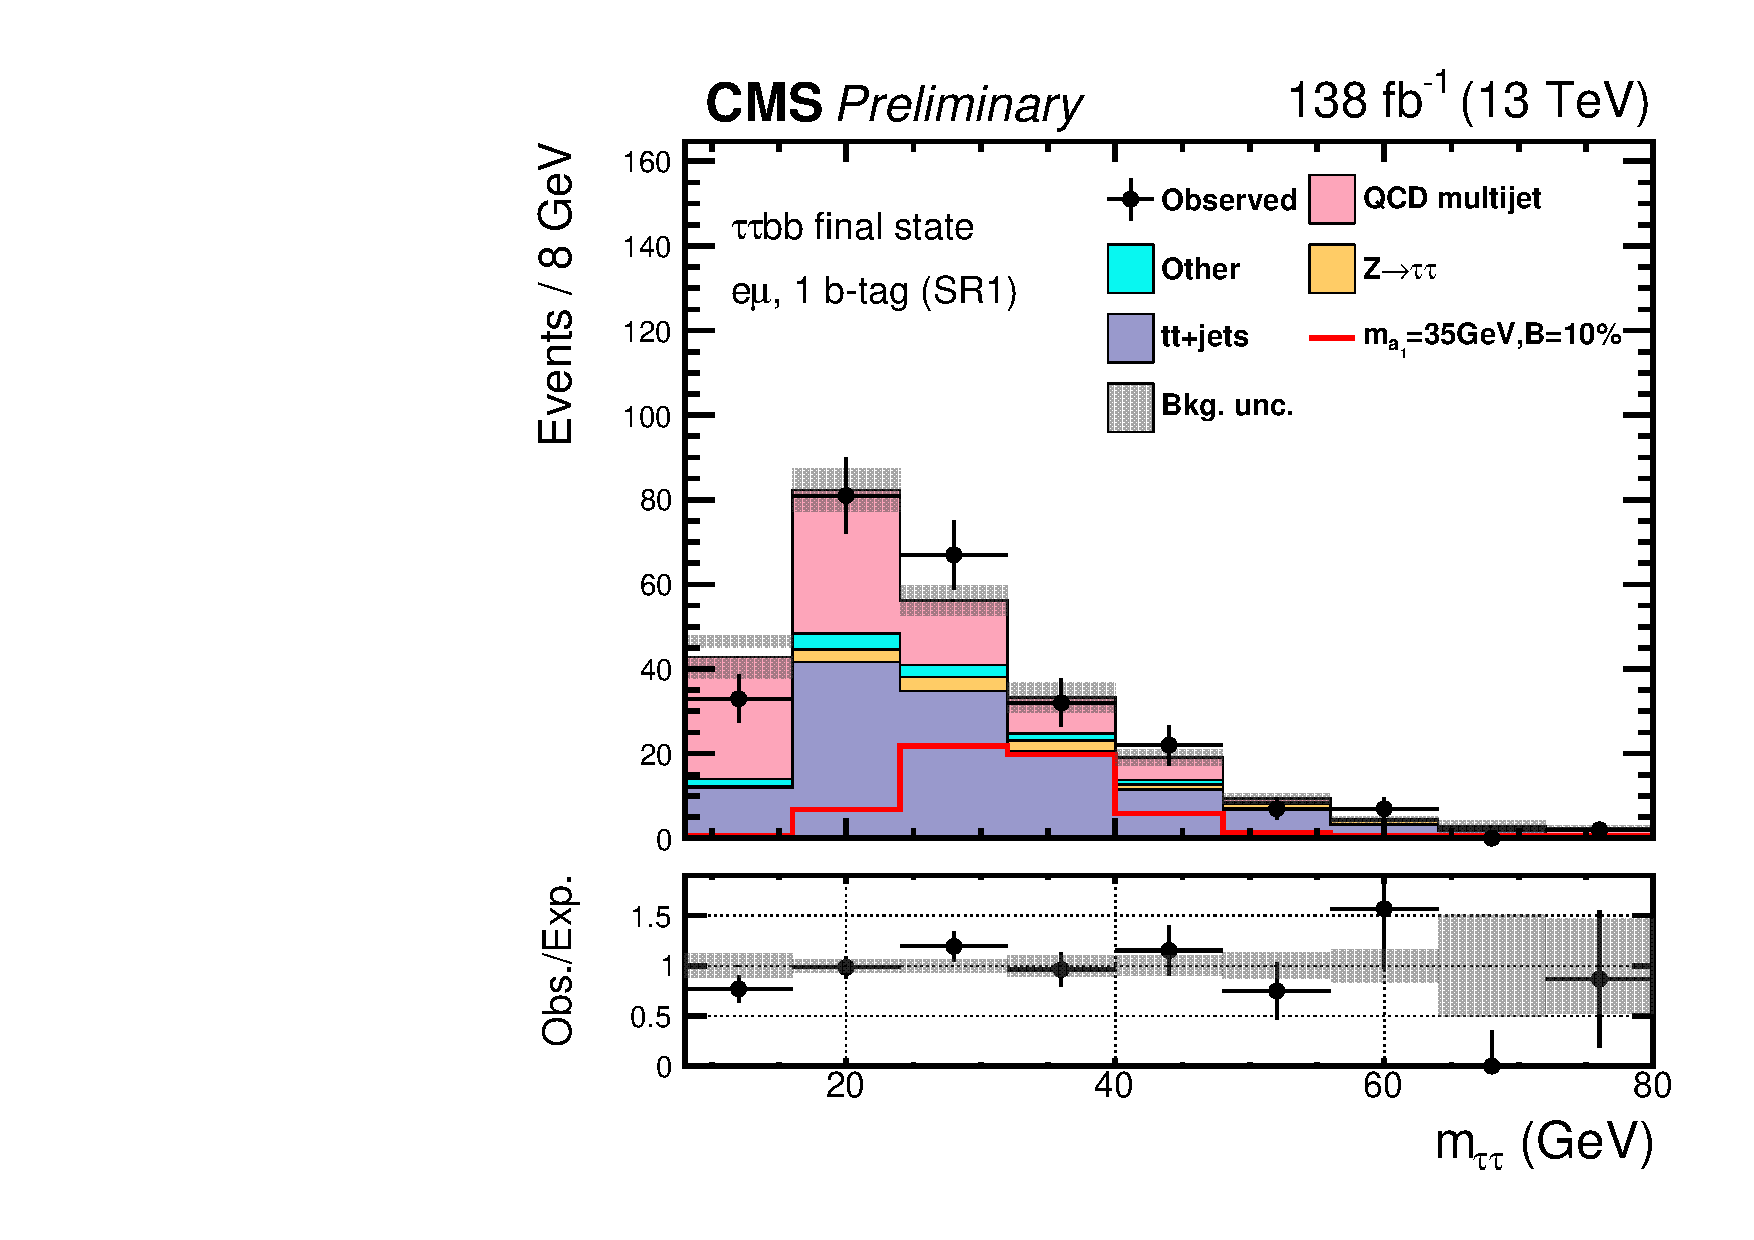
\includegraphics[width=0.32\textwidth]{figures/ch-10-results/em_all_1_post_prelim-yes.pdf}
        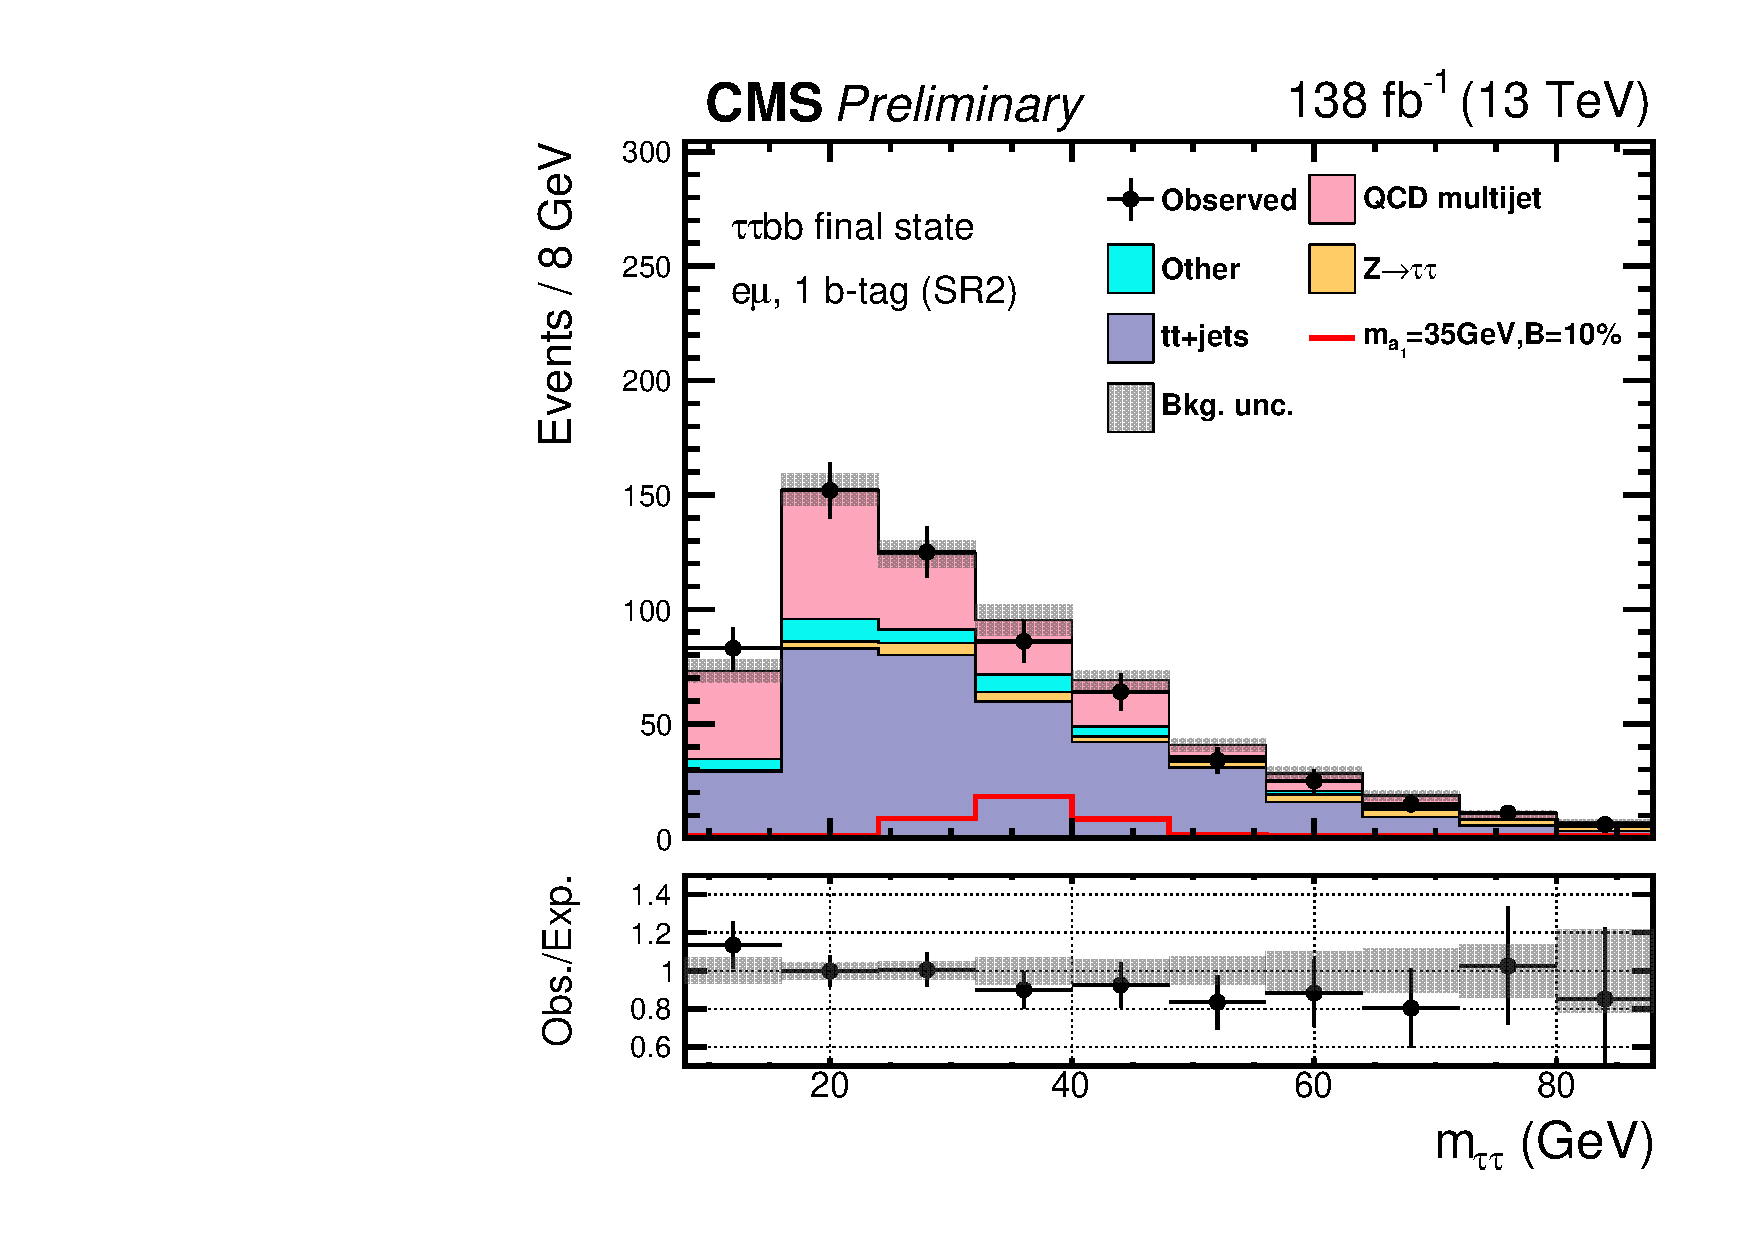
\includegraphics[width=0.32\textwidth]{figures/ch-10-results/em_all_2_post_prelim-yes.pdf}
        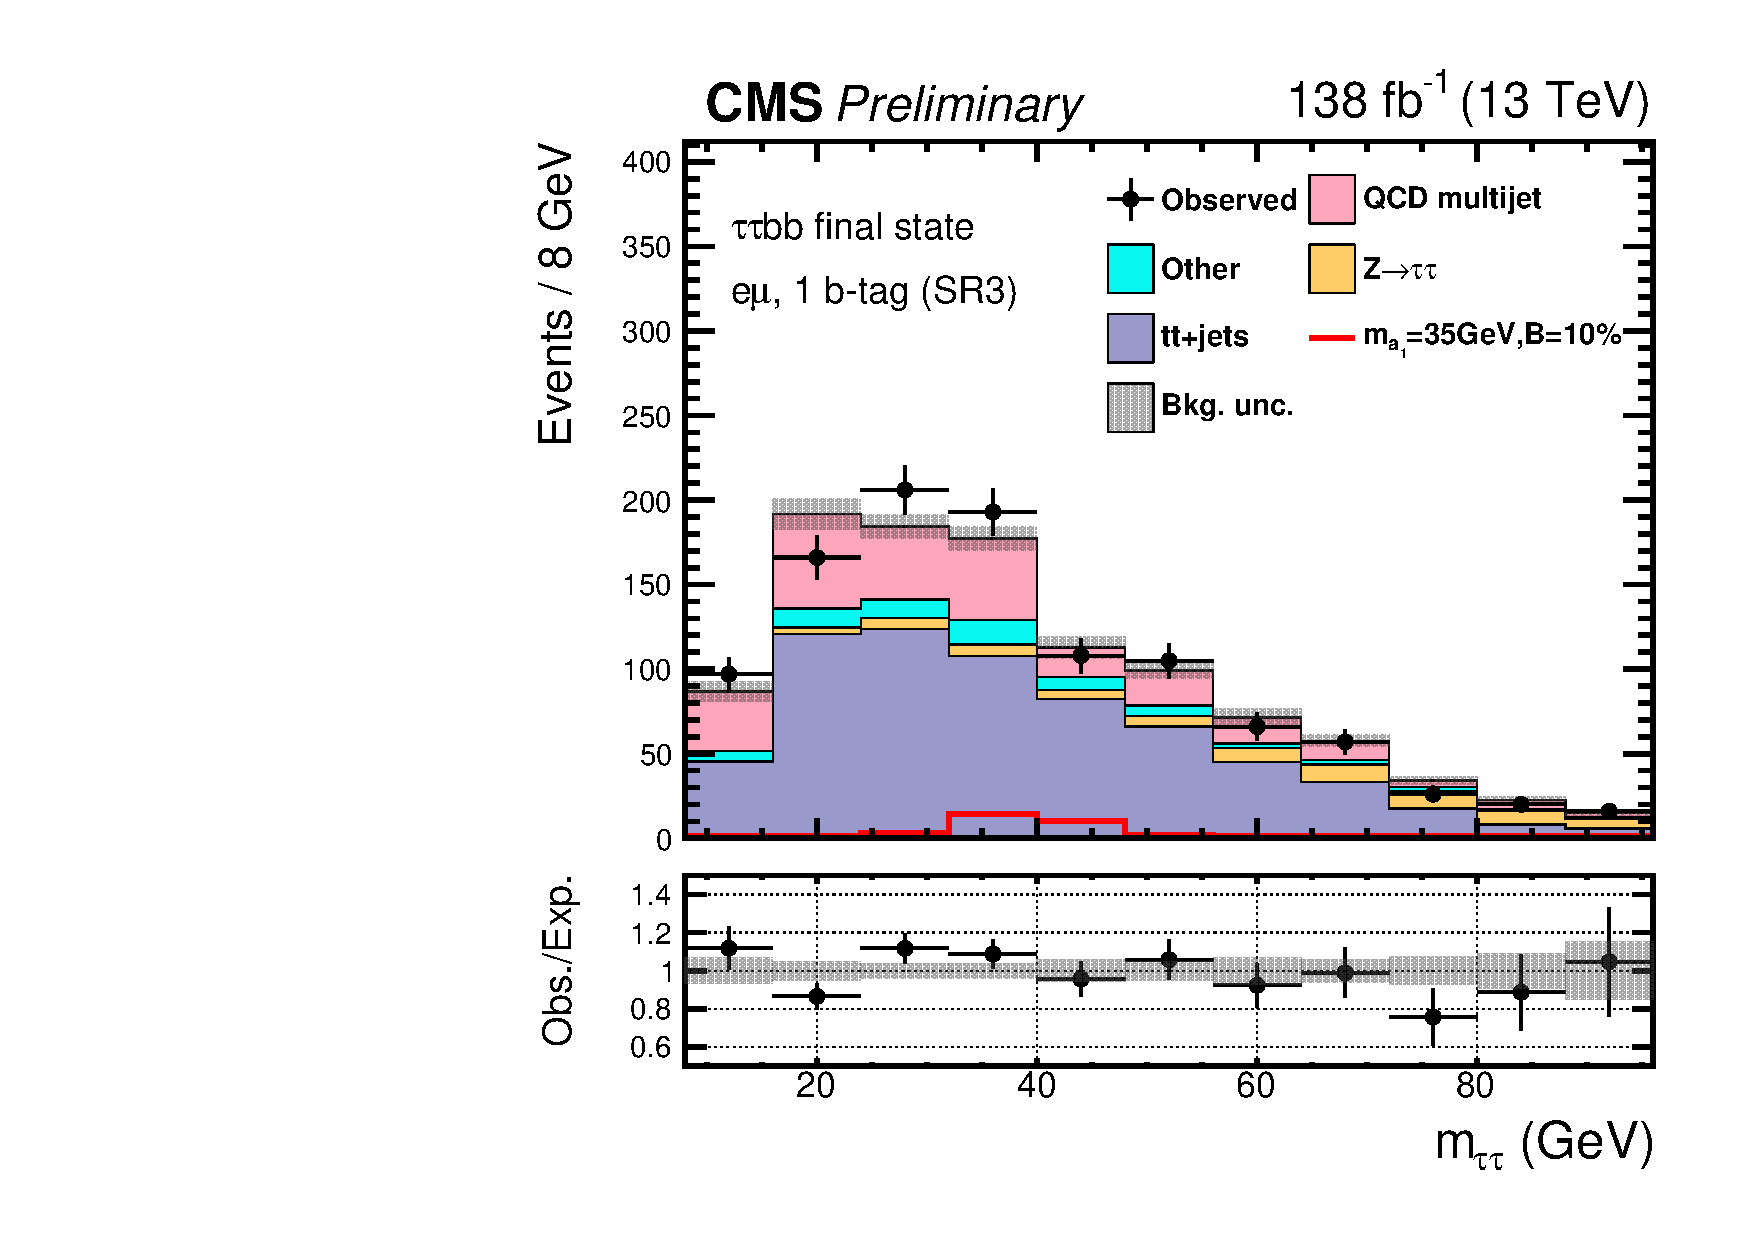
\includegraphics[width=0.32\textwidth]{figures/ch-10-results/em_all_3_post_prelim-yes.pdf}\\
        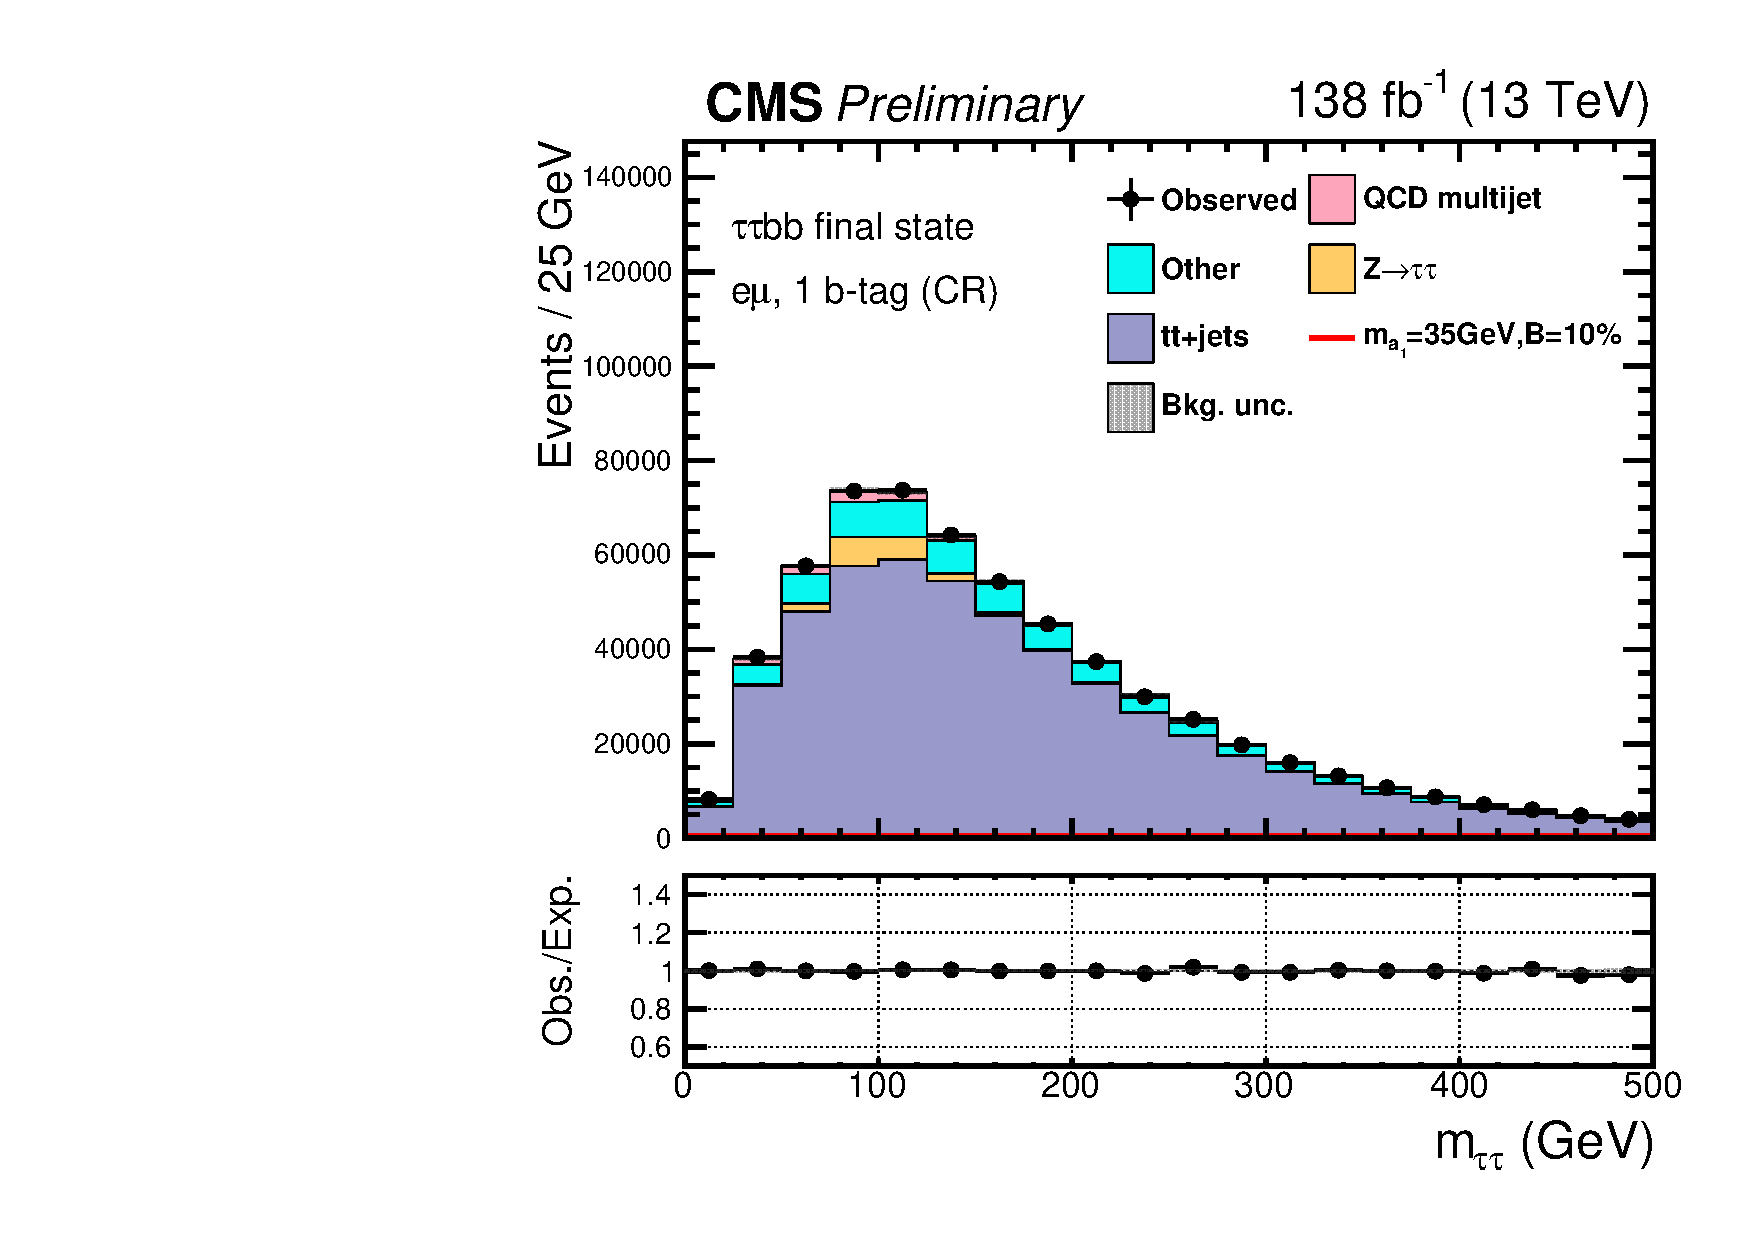
\includegraphics[width=0.32\textwidth]{figures/ch-10-results/em_all_4_post_prelim-yes.pdf}
        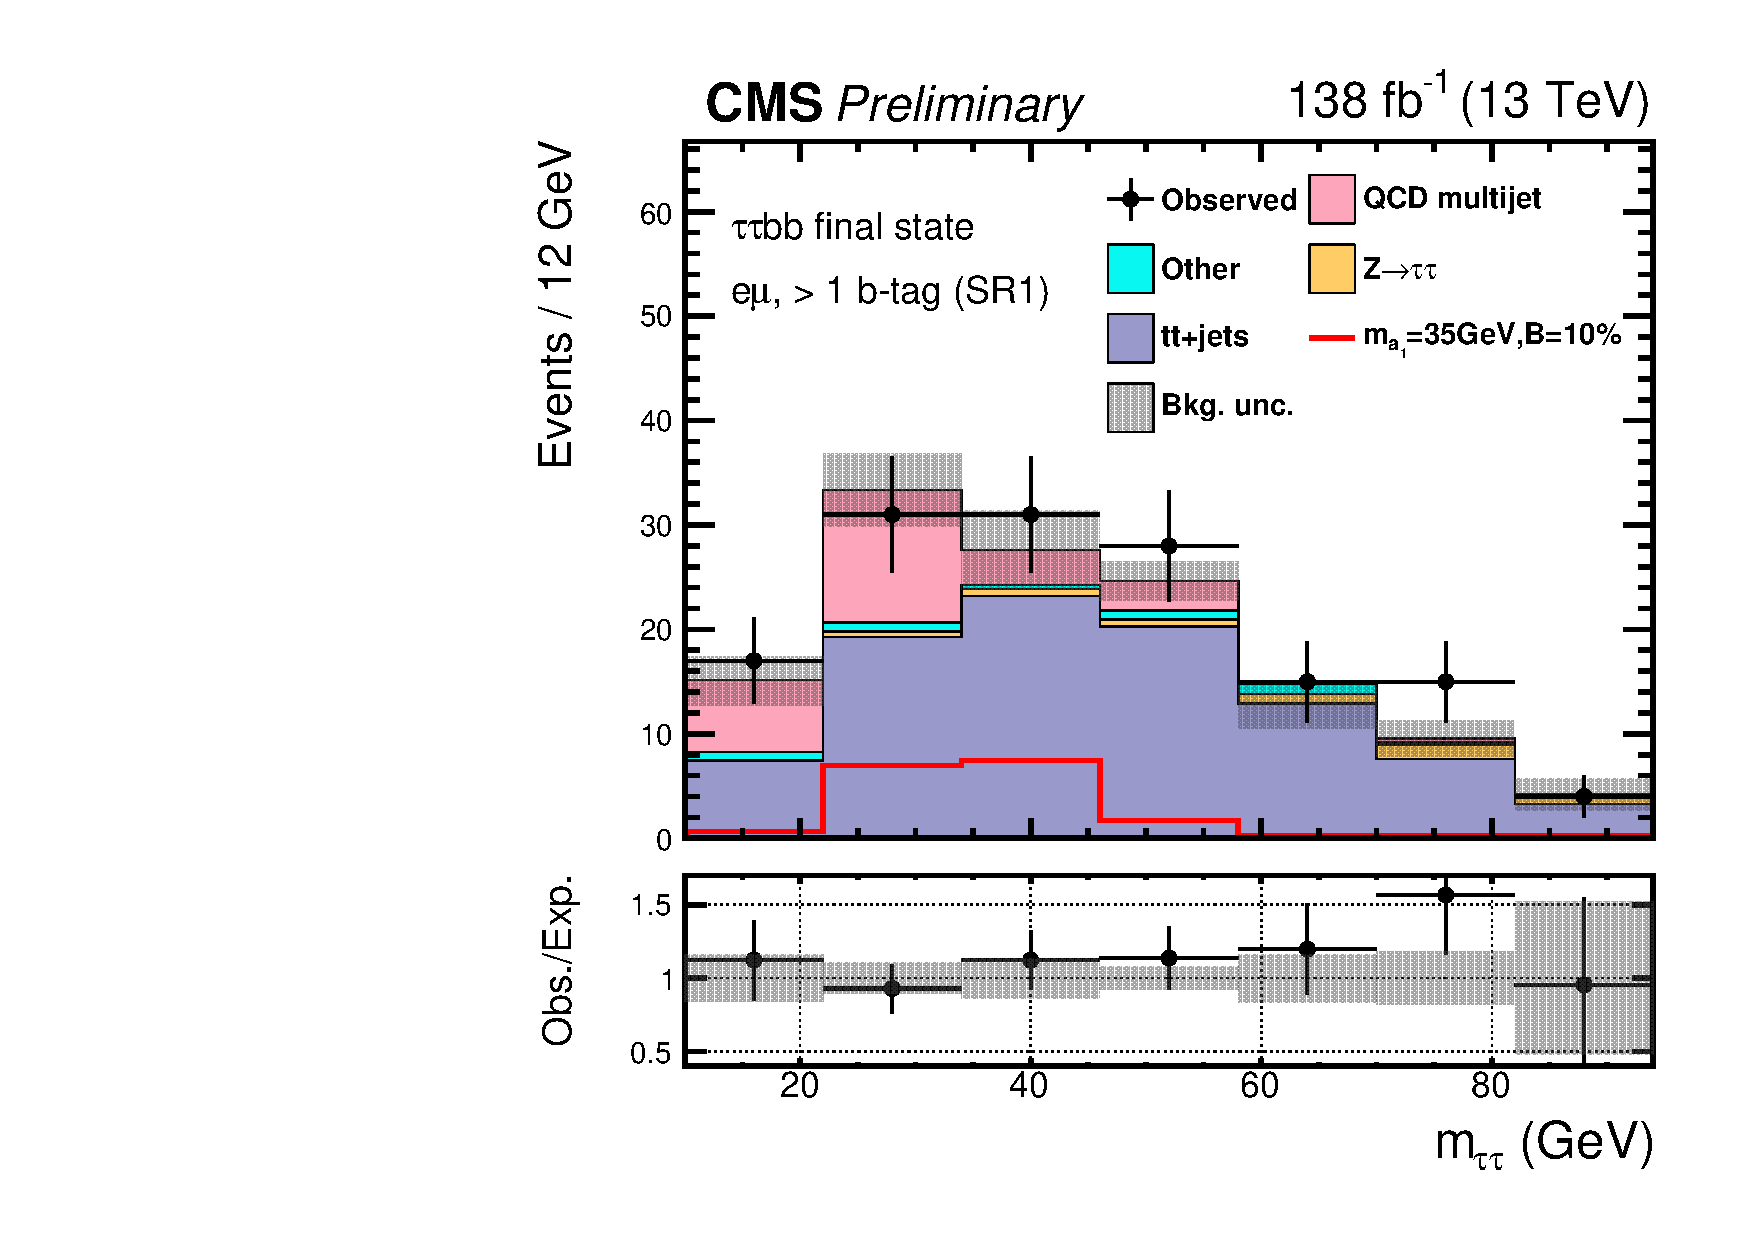
\includegraphics[width=0.32\textwidth]{figures/ch-10-results/em_all_5_post_prelim-yes.pdf}
        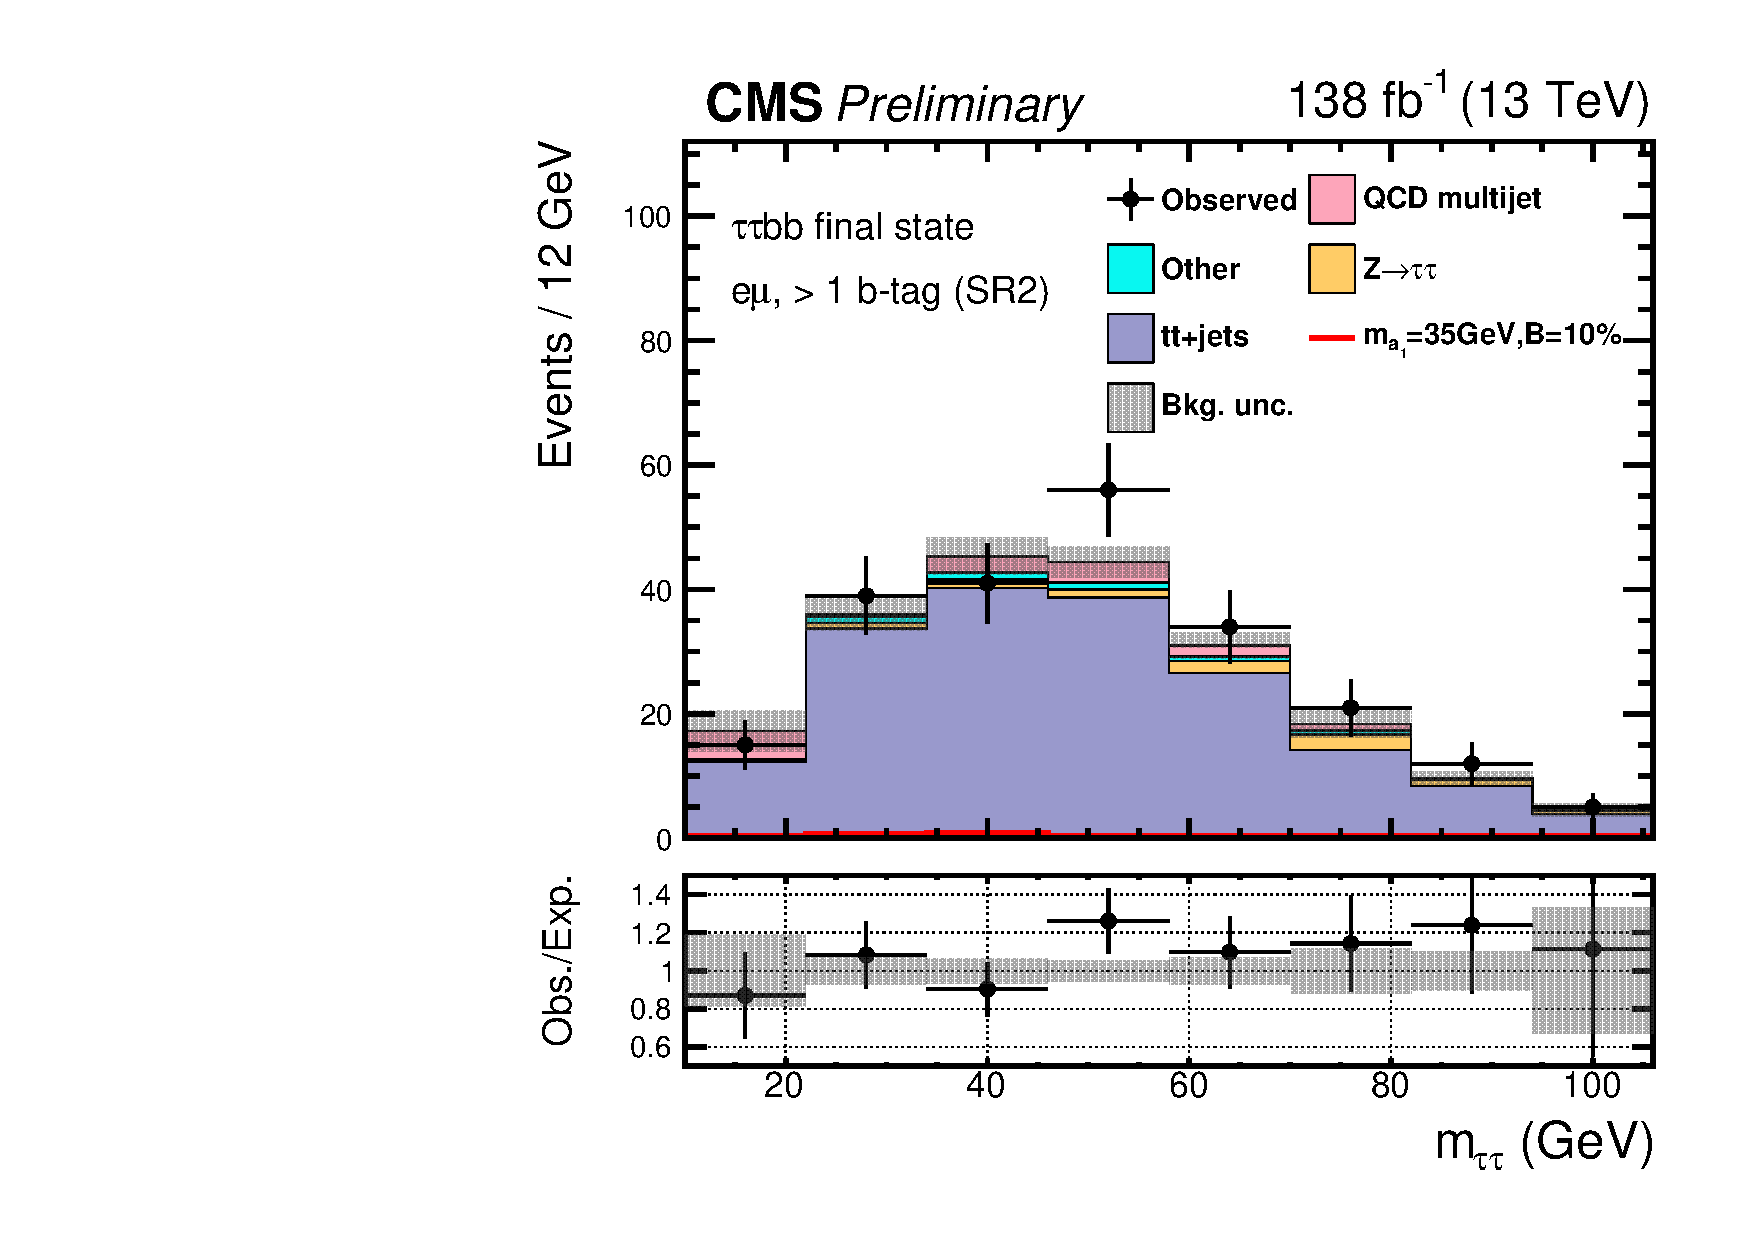
\includegraphics[width=0.32\textwidth]{figures/ch-10-results/em_all_6_post_prelim-yes.pdf}\\
        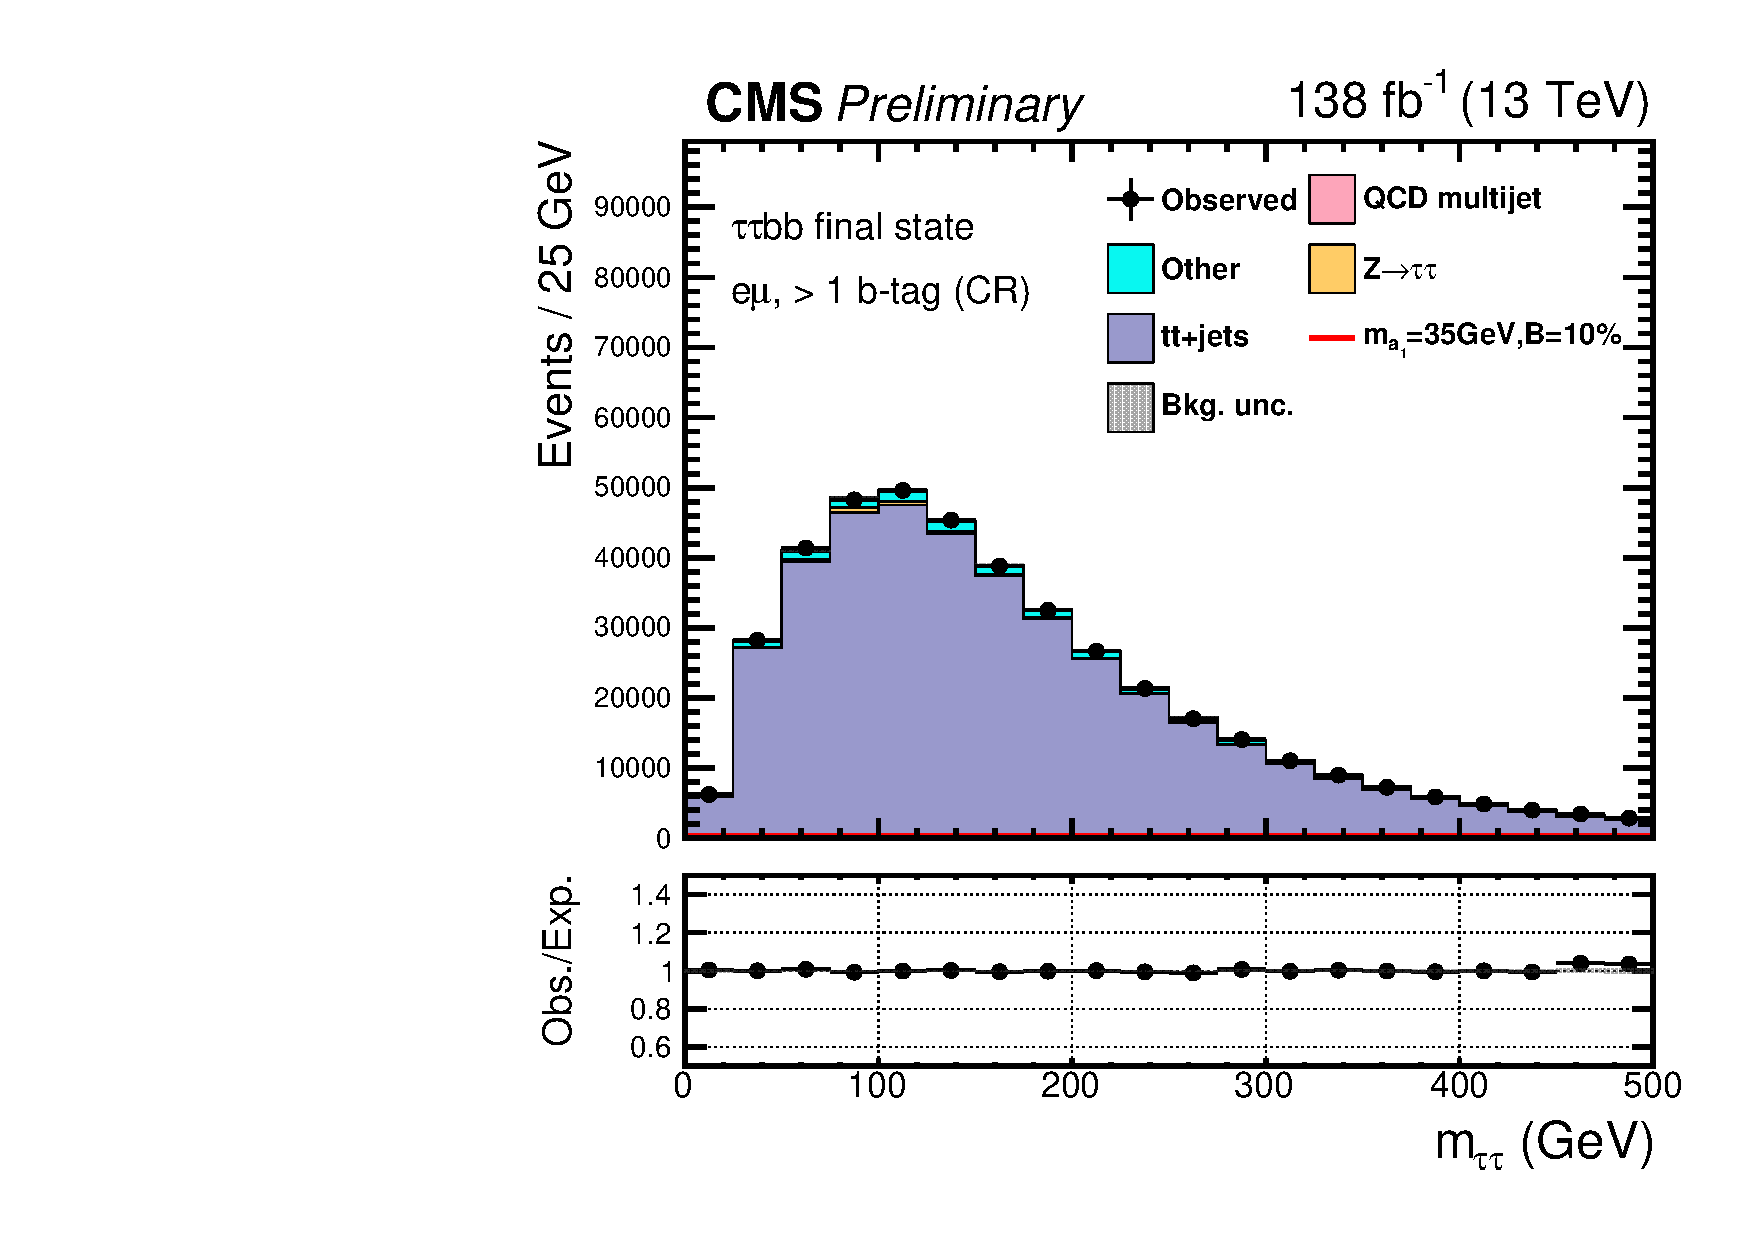
\includegraphics[width=0.32\textwidth]{figures/ch-10-results/em_all_7_post_prelim-yes.pdf}
    \end{center}
    \caption[Postfit final observed and expected $m_{\tau\tau}$ distributions in the $e\mu$ channel.]{Postfit final observed and expected $m_{\tau\tau}$ distributions, and the observed/expected ratios, in the $e\mu$ channel \cite{CMS-AN-20-213}. Events are divided into the 1 b-tag jet signal regions (SR1, SR2, and SR3) (\textit{top row}), 1 b-tag jet control region (CR) (\textit{middle row}), 2 b-tag jet signal regions (SR1 and SR2) (\textit{middle row}), and 2 b-tag jet control region (CR) (\textit{bottom row}). Statistical and systematic sources of uncertainties in the expected events are added in quadrature and labeled ``Bkg. unc" (\textit{shaded gray}). The $t\bar{t}$+jets process(\textit{purple}) is a major background, and in the signal regions the QCD multijet (\textit{pink}) is also a major background. TFor illustrative purposes, the beyond-Standard Model signal yield from $h\rightarrow aa bb\tau\tau$ is shown for the pseudoscalar mass hypothesis $m_a = 35$ GeV, assuming a branching fraction $B(h \rightarrow aa \rightarrow bb\tau\tau) = 10\%$ (\textit{red line}).}
    \label{fig:results_mtt_postfit_emall}
\end{figure}


The 95\% CL expected and observed exclusion limits on the signal strength of the branching fraction $B(h \rightarrow aa \rightarrow bb\tau\tau)$ as a function of the pseudoscalar mass $m_a$ ranging from 12 GeV to 60 GeV, are shown for the three $\tau\tau$ channels and all three channels combined in Fig. \ref{fig:results_limits}. The limits are shown as percentages and normalized to the production cross-section of the Standard Model Higgs boson. No excess of events above the Standard Model expectations is observed. In the limits for the three $\tau\tau$ channels combined, expected (observed) limits range from 1.4 to 5.6\% (1.7 to 7.6\%) for pseudoscalar masses between 12 and 60 GeV.


The $e\mu$ channel is the only channel that has signal sensitivity to the $m_a = 12$ GeV pseudoscalar mass hypothesis, because the minimum required spatial separation $\Delta R = \sqrt{(\Delta \eta)^2 + (\Delta \phi)^2}$ between the two $\tau$ legs is smaller than the other two channels ($\Delta R < 0.3$ for $e\mu$, compared to $\Delta R < 0.4$ for the other two channels). This decreased $\Delta R$ requirement results in better signal acceptance for low mass signals for the $e\mu$ channel. The $\mu\tau_{h}$ and $e\tau_{h}$ channels are most sensitive to the intermediate mass points studied, since the analysis targets a resolved signature: at low mass points, the tau legs are boosted, and at high mass points, the $m_{\tau\tau}$ distributions in signal have larger overlap with background distributions. In the combination of the three $\tau\tau$ channels, the limit for $m_a = 12$ GeV comes only from the $e\mu$ channel, and the best sensitivity is attained at intermediate mass points around $m_a = 20$ GeV to 45 GeV.


\begin{figure}[h!]
    \begin{center}
        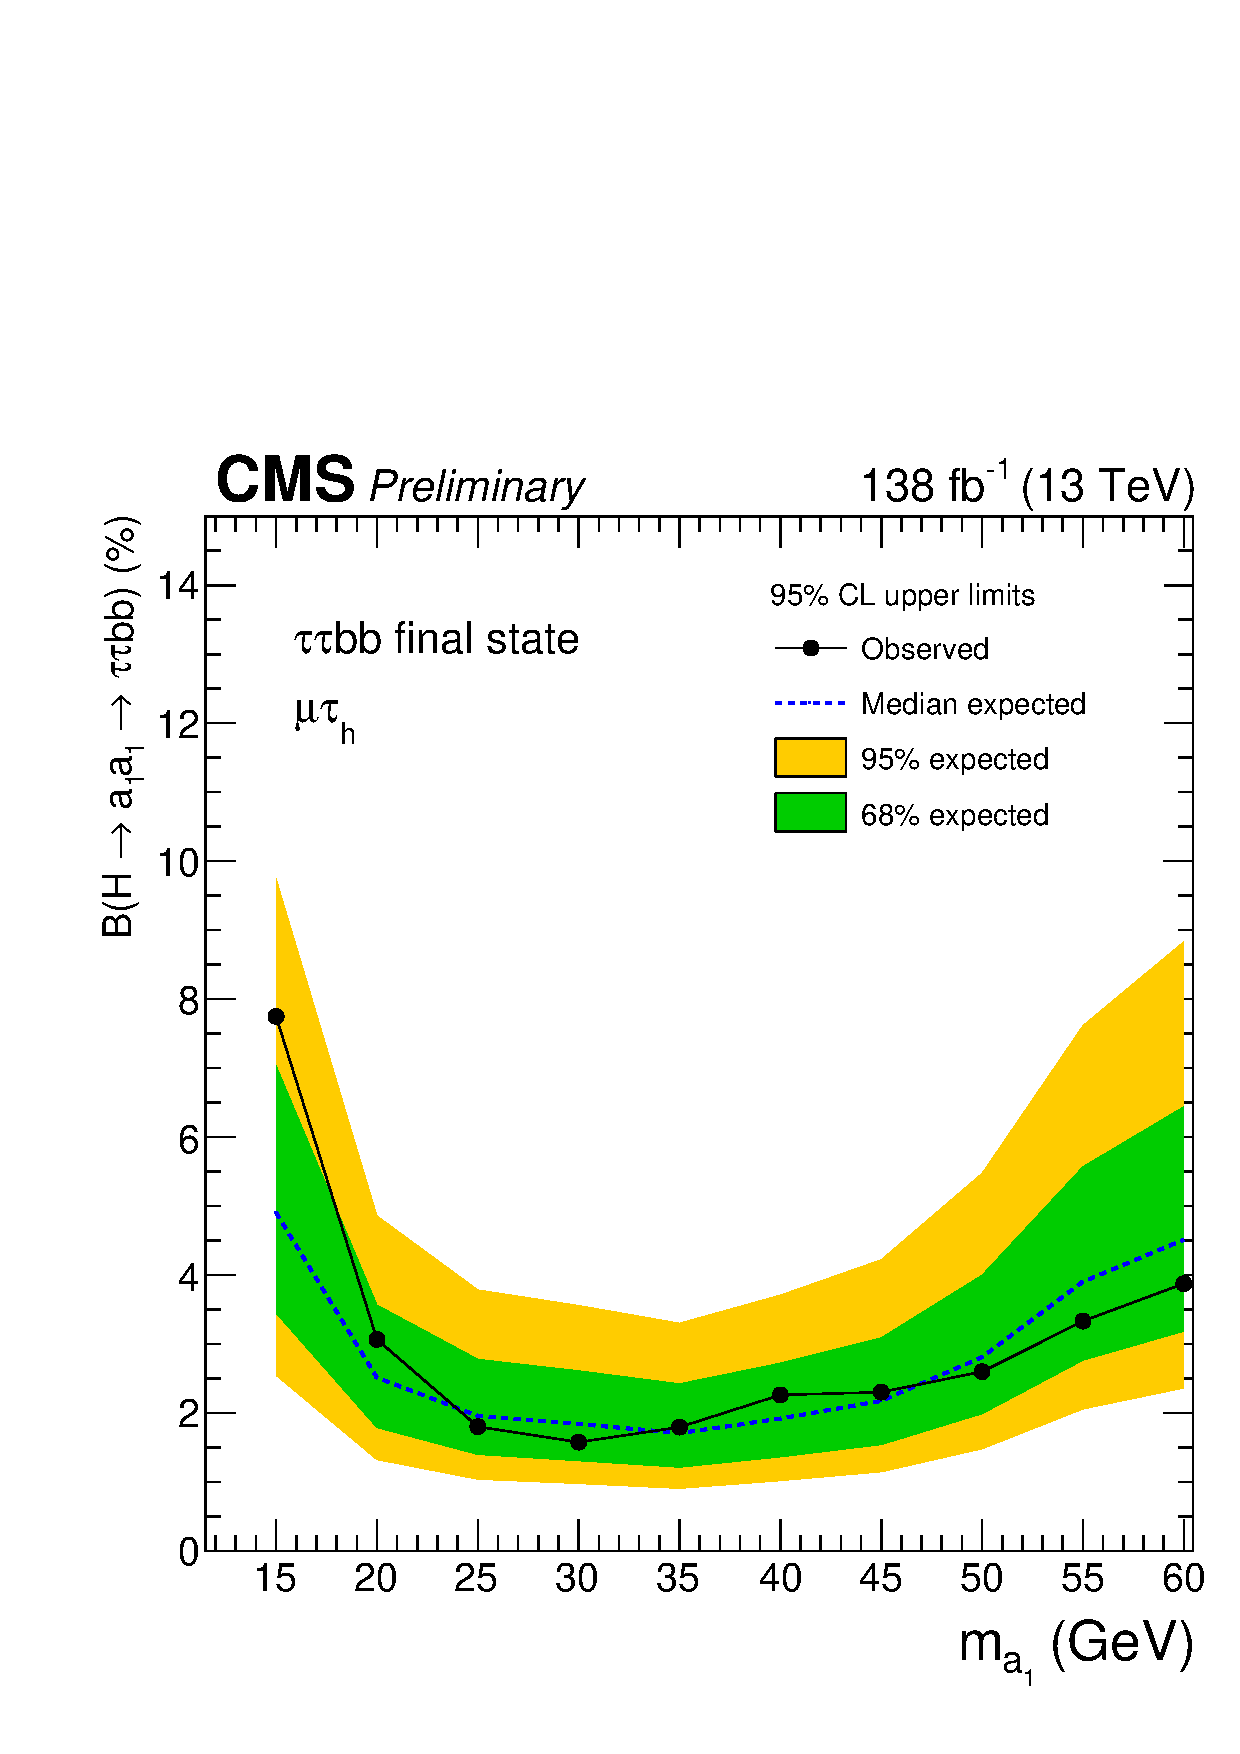
\includegraphics[width=0.45\textwidth]{figures/ch-10-results/Limit_mt_prelim.pdf}
        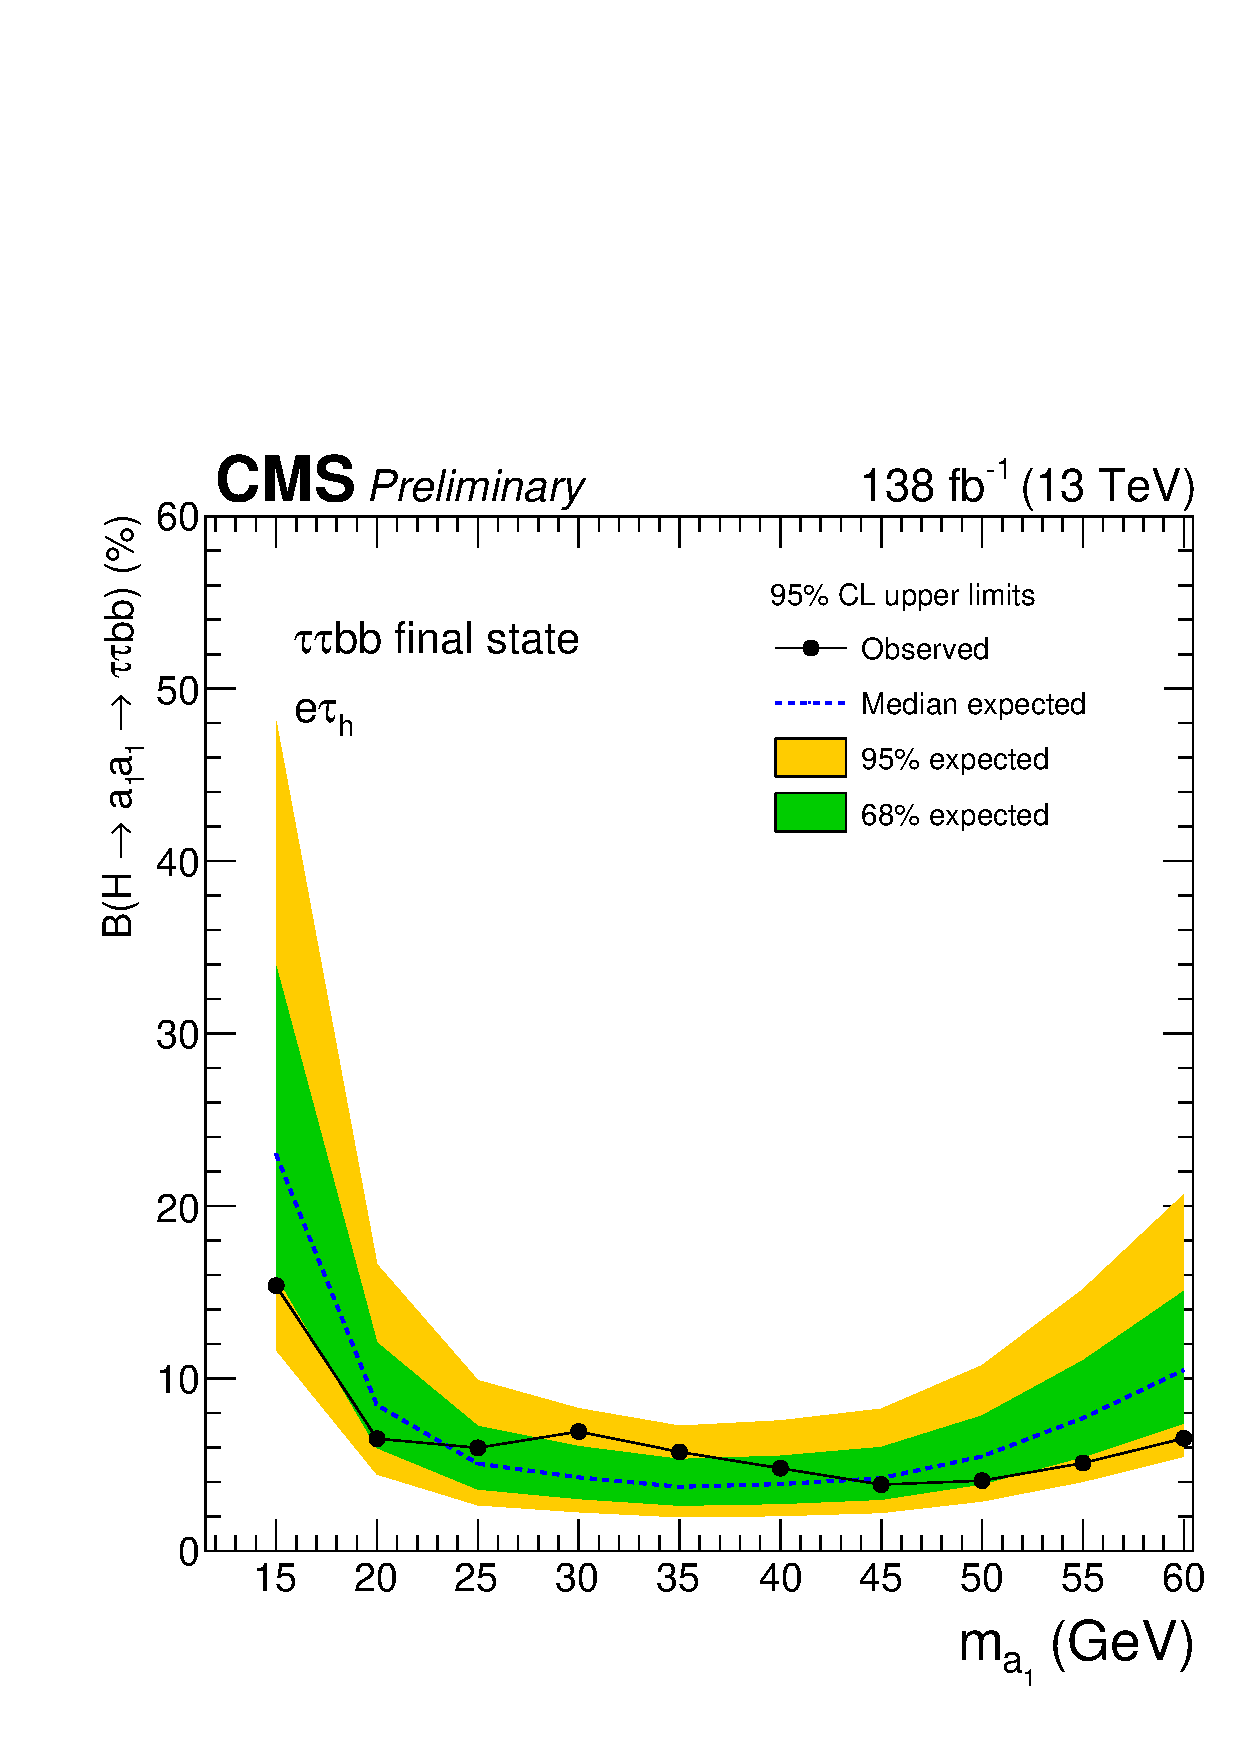
\includegraphics[width=0.45\textwidth]{figures/ch-10-results/Limit_et_prelim.pdf}\\
        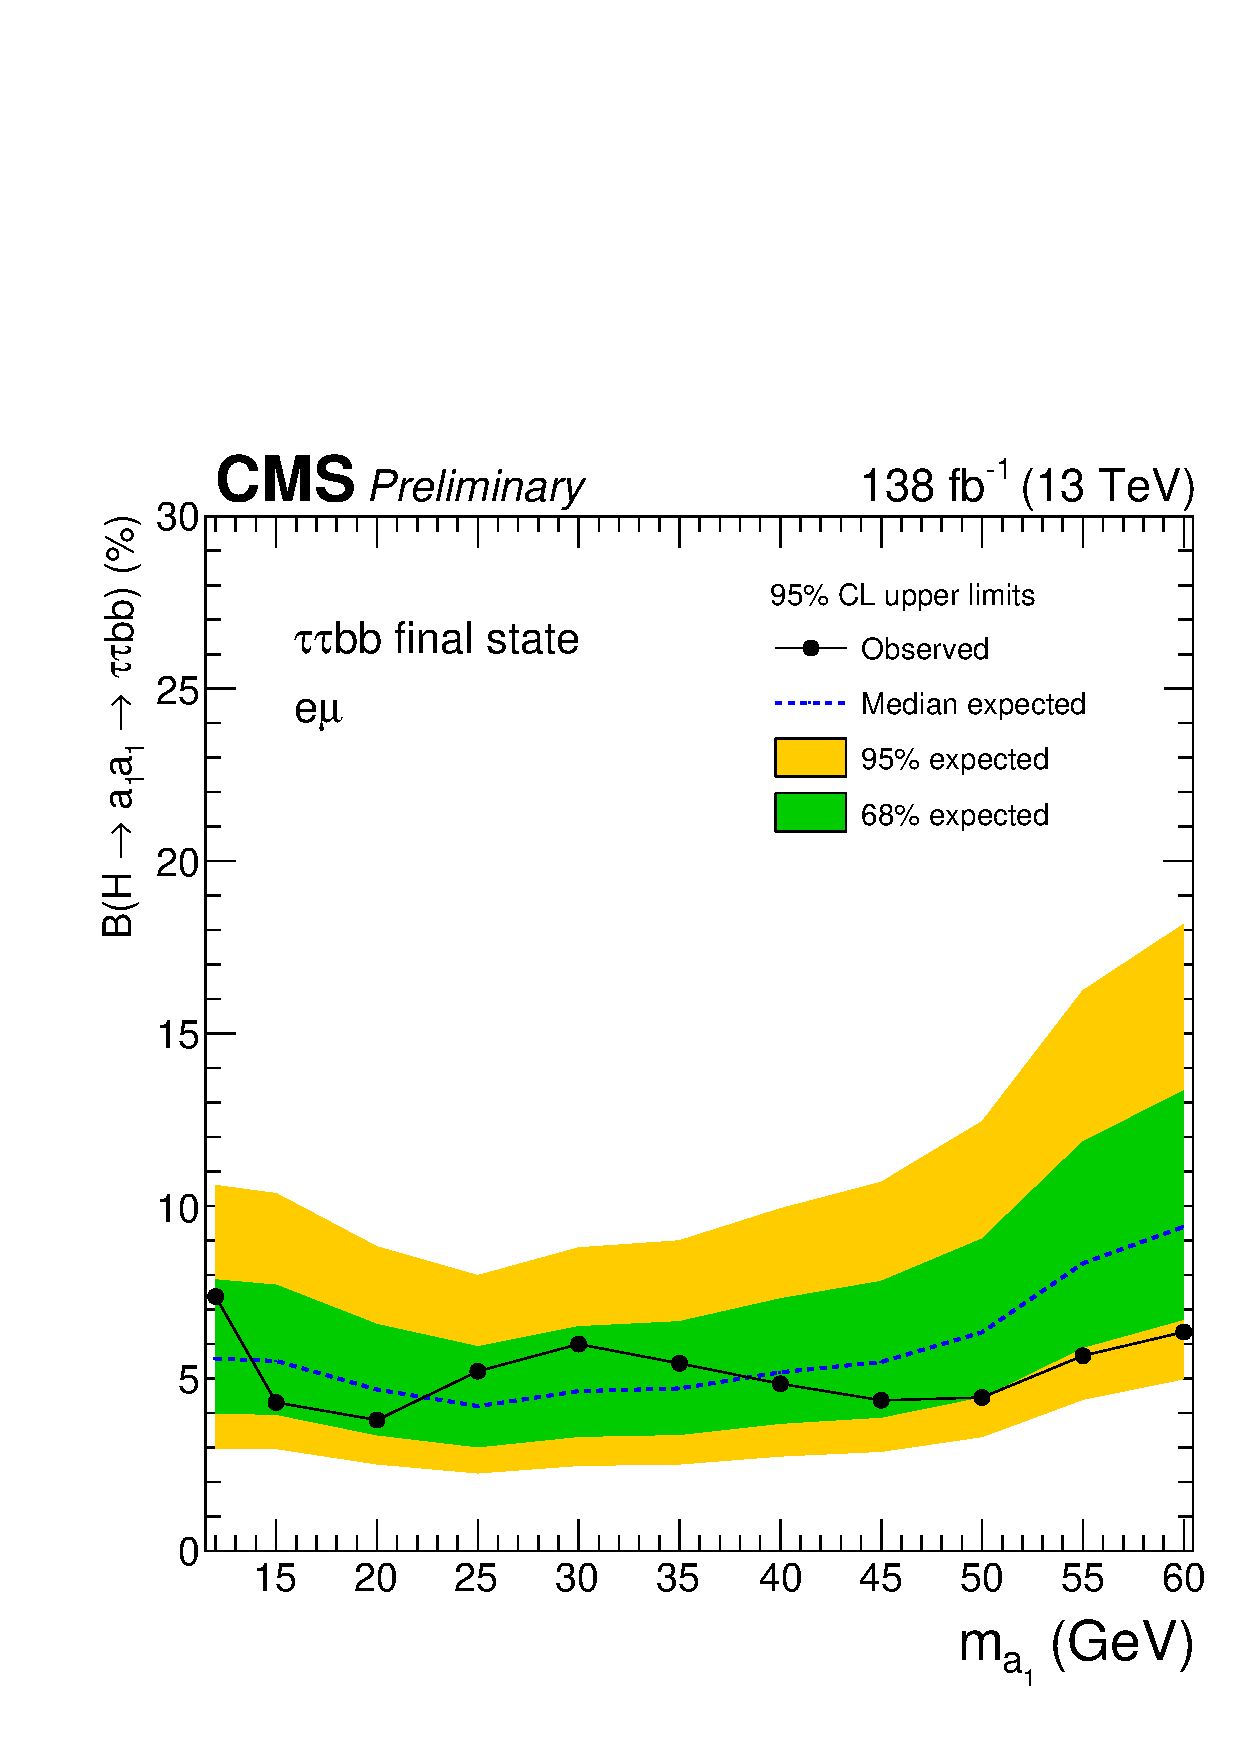
\includegraphics[width=0.45\textwidth]{figures/ch-10-results/Limit_em_prelim.pdf}
        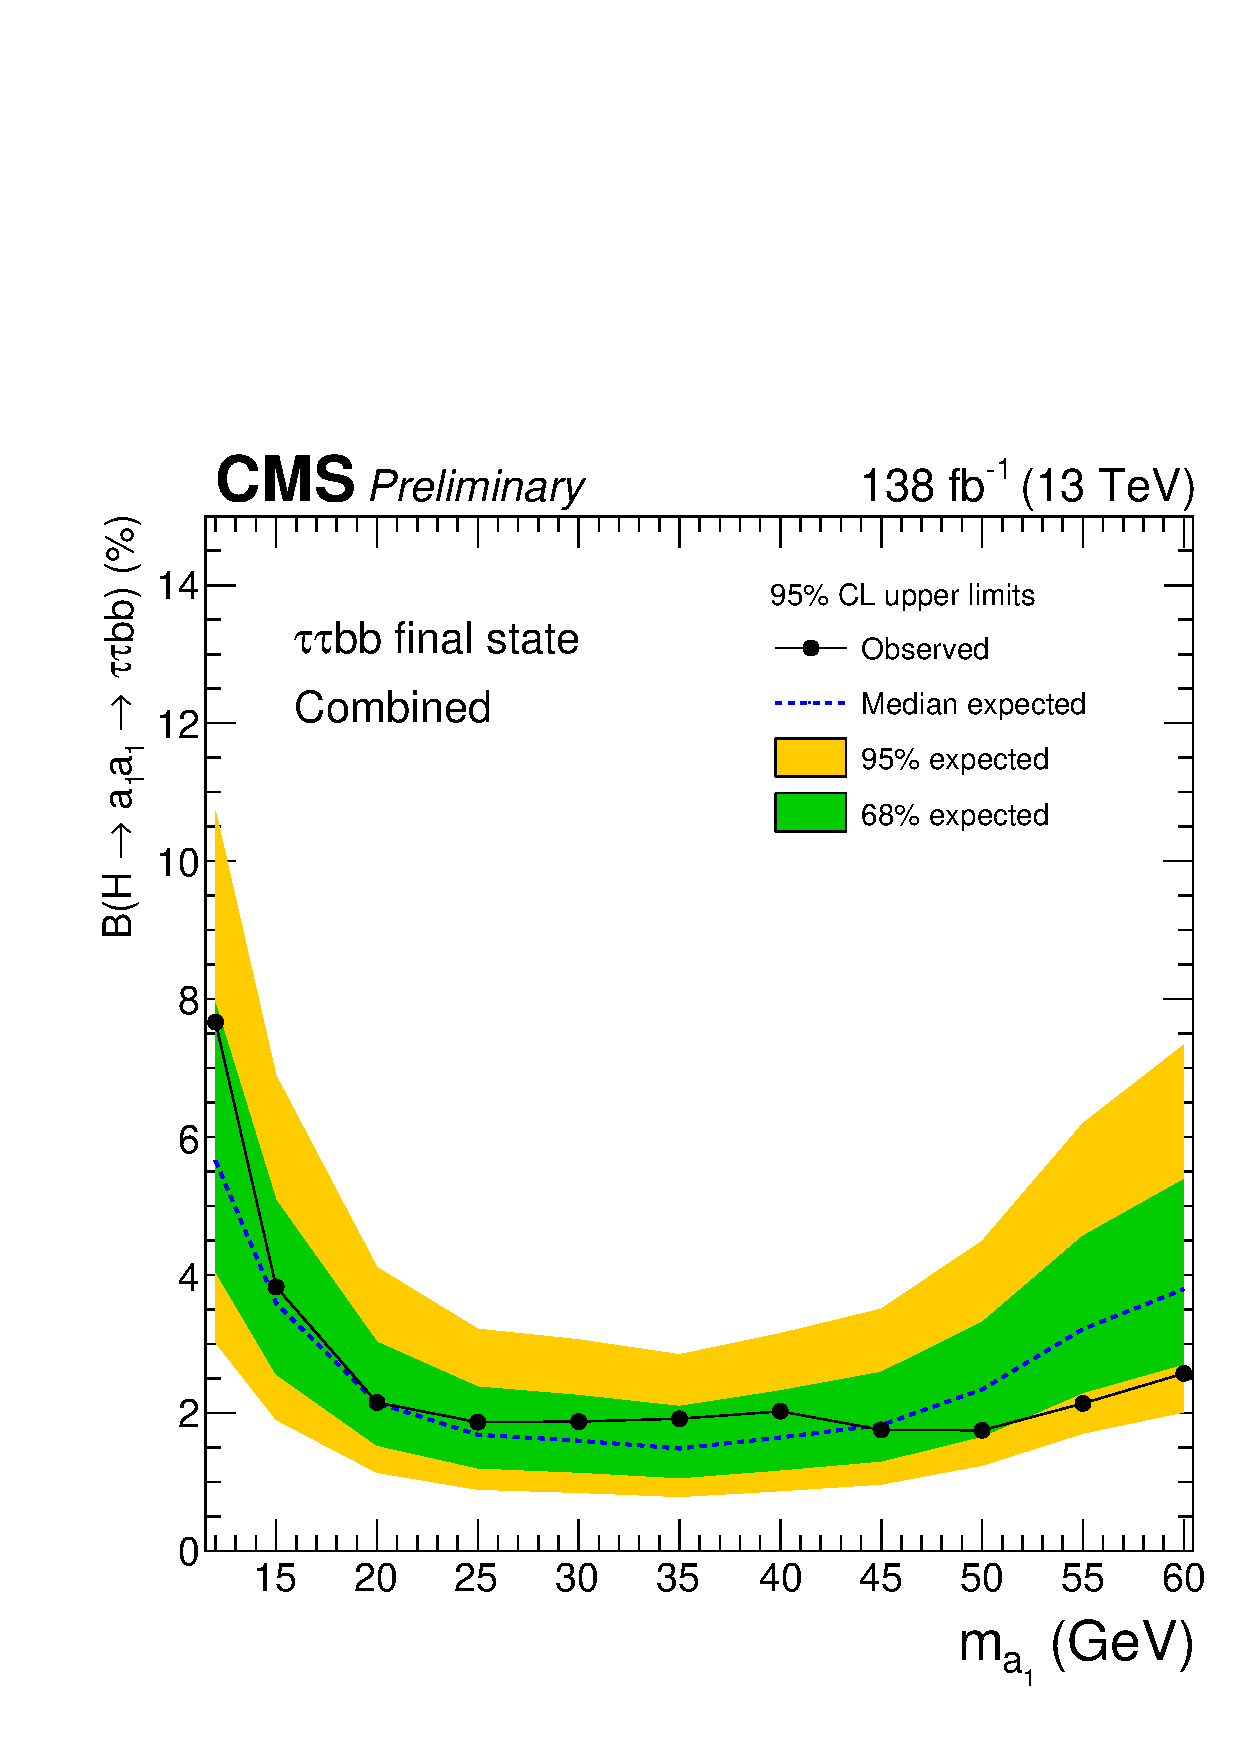
\includegraphics[width=0.45\textwidth]{figures/ch-10-results/Limit_all_prelim.pdf}
    \end{center}
    \caption[Observed 95\% CL exclusion limits (\textit{black, solid lines}) and expected 95\% CL and 68\% CL limits (\textit{shaded yellow and green}) on the branching fraction B($h\rightarrow aa\rightarrow bb\tau\tau$) in percentages, assuming the Standard Model production for the 125 GeV Higgs ($h$). Limits are shown for the $\mu\tau_{h}$ channel (\textit{top left}), the $e\tau_{h}$ channel (\textit{top right}), and the $e\mu$ channel (\textit{bottom left}), and lastly the combination of all three channels (\textit{bottom right}) The dataset corresponds to 138 fb$^{-1}$ of data collected in the years 2016-2018 at a center-of-mass energy 13 TeV.]{Observed 95\% CL exclusion limits (\textit{black, solid lines}) and expected 95\% CL and 68\% CL limits (\textit{shaded yellow and green}) on the branching fraction B($h\rightarrow aa\rightarrow bb\tau\tau$) in percentages, assuming the Standard Model production for the 125 GeV Higgs ($h$). Limits are shown for the $\mu\tau_{h}$ channel (\textit{top left}), the $e\tau_{h}$ channel (\textit{top right}), and the $e\mu$ channel (\textit{bottom left}), and lastly the combination of all three channels (\textit{bottom right}) \cite{CMS-AN-20-213}. The dataset corresponds to 138 fb$^{-1}$ of data collected in the years 2016-2018 at a center-of-mass energy 13 TeV. Only the $e\mu$ channel has sensitivity to the mass hypothesis $m_a = 12$ GeV. The best sensitivity is attained at intermediate mass points.}
    \label{fig:results_limits}
\end{figure}

To set limits on the branching fraction of the 125 GeV Higgs to the two pseudoscalars, $B(h \rightarrow aa)$, we interpret the results in four types of 2HDM+S, which were introduced in Section \ref{section:theory-2HDM}. In 2HDM+S, the theorized branching fraction of the pseudoscalars depends on the 2HDM+S model type, the pseudoscalar mass $m_a$, and the ratio of the two Higgs doublets' vacuum expectation values $\tan\beta$. In Type I models, the branching fraction is independent of $\tan\beta$, while in Types II, III, and IV, it is a function of $m_a$ and $\tan\beta$. Limits for the $bb\tau\tau$ final state as a function of $m_a$ for 2HDM+S Type I (valid for all $\tan\beta$ values), Type II with $\tan\beta = 2.0$, Type III with $\tan\beta = 2.0$, and Type IV with $\tan\beta = 0.6$ are overlaid and shown in Fig. \ref{fig:bbtautau_only_limits}.


\section{Combination with \texorpdfstring{$bb\mu\mu$}{bbmumu} final state}
\label{section:combination-procedure-with-bbmumu}
Results from this analysis for the $h \rightarrow aa \rightarrow bb\tau\tau$ final state are combined with the analysis for the $h \rightarrow aa \rightarrow bb\mu\mu$ final state \cite{CMS-AN-21-058-bbmumu}. While the predicted branching ratio for $aa \rightarrow bb\mu\mu$ is comparatively small, the $bb\mu\mu$ final state has competitive results due to the excellent di-muon resolution measured by CMS. The $bb\mu\mu$ analysis uses an unbinned fit to the data using the di-muon mass $m_{\mu\mu}$ distribution. Details can be found in \cite{CMS-AN-21-058-bbmumu}.

Combining the results is possible since the $bb\tau\tau$ analysis explicitly rejects events with extra leptons, so there is no overlap between the events studied in the $bb\tau\tau$ analysis and the $bb\mu\mu$ analysis. In the statistical combination, several systematic uncertainties are treated as correlated: the integrated luminosity normalization, the b-tagging scale factor, the scale factors related to muon reconstruction, identification, and trigger efficiencies, the inefficiency in the ECAL trigger readout, and the theoretical uncertainties related to signal modeling.

Since the results in both final states are statistically limited, the combination benefits from the additional data. For $m_a = 35$ GeV, all systematic uncertainties amount to around 6\% of the total uncertainty, with the dominant systematic uncertainties coming from jet energy systematics in the $bb\mu\mu$ final state, theoretical uncertainties in the signal, and uncertainties in the QCD multijet backgrounds in the $e\mu$ channel of the $bb\tau\tau$ final state.

The mass distributions of the di-muon and di-tau objects ($m_{\mu\mu}$ and $m_{\tau\tau}$) are compared to the data in a combined maximum likelihood fit to derive upper limits on $B(h\rightarrow aa)$. The observed limits at 95\% CL on $B(h \rightarrow aa)$ for different 2HDM+S scenarios, are shown for the search for $h \rightarrow aa \rightarrow bb\mu\mu$ in Fig. \ref{fig:bbmumu_only_limits}, and the combined analyses $h \rightarrow aa \rightarrow bb\ell\ell$ in Fig. \ref{fig:results_limits_combined}. 

\begin{figure}[ht]
  \begin{subfigure}{0.45\textwidth}
    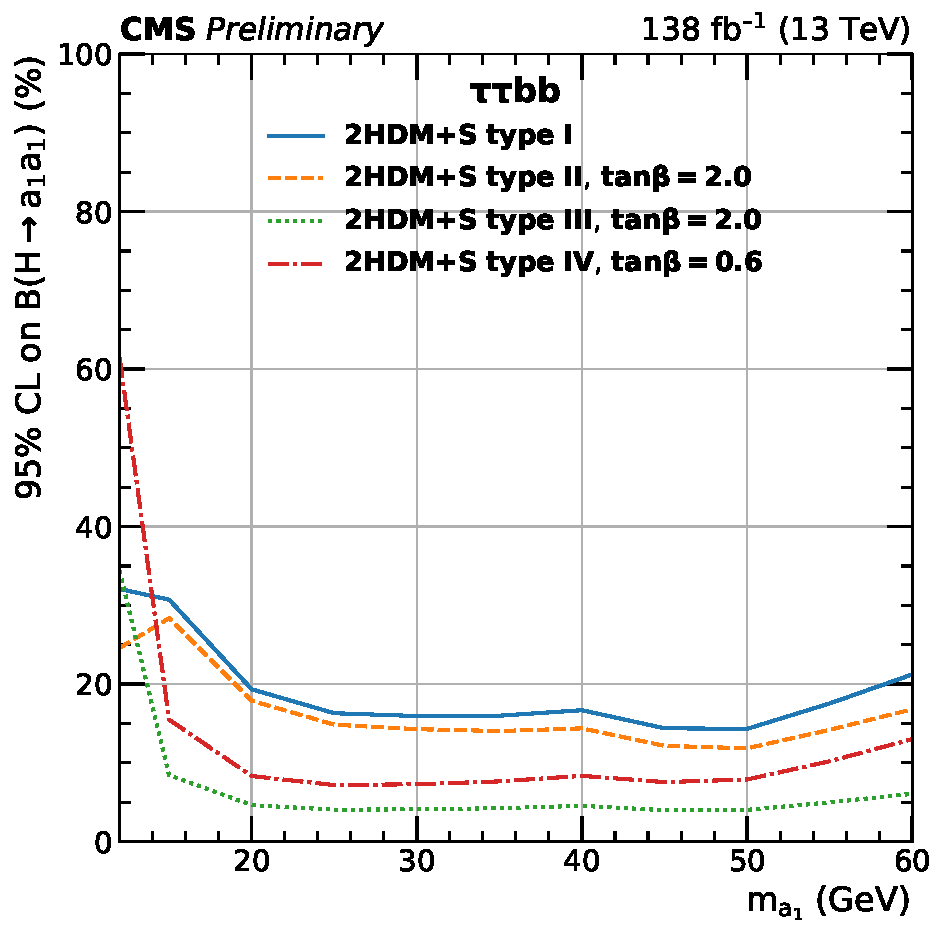
\includegraphics[width=1.0\textwidth]{figures/ch-10-results/HAA_bbtt_all_prelim.pdf}
    \caption{$bb\tau\tau$ final state.}
    \label{fig:bbtautau_only_limits}
\end{subfigure}
\hfill
\begin{subfigure}{0.45\textwidth}
    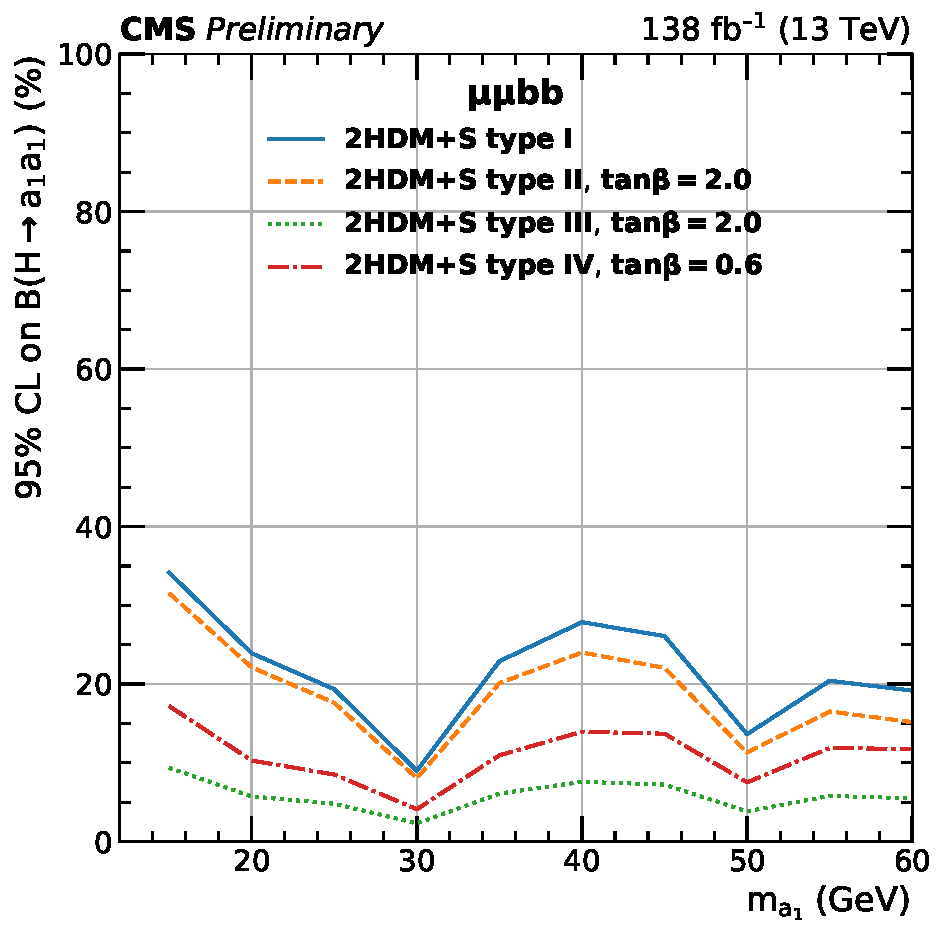
\includegraphics[width=1.0\textwidth]{figures/ch-10-results/HAA_bbmm_all_prelim.pdf}
      \caption{$bb\mu\mu$ final state.}
      \label{fig:bbmumu_only_limits}
  \end{subfigure}
  \caption[Observed 95\% CL upper limits on B$(h \rightarrow aa)$ in \%, for the $bb\tau\tau$ final state (\textit{left}) and $bb\mu\mu$ final state (\textit{right}) using the full Run 2 integrated luminosity of 138 fb$^{-1}$ in 2HDM+S type I (\textit{blue}), type II with $\tan\beta = 2.0$ (\textit{orange dashed}), type III with $\tan\beta = 2.0$ (\textit{dotted green}), and type IV with $\tan\beta = 0.6$ (\textit{red dashed}).]{Observed 95\% CL upper limits on B$(h \rightarrow aa)$ in \%, for the $bb\tau\tau$ final state (\textit{left}) and $bb\mu\mu$ final state (\textit{right}) using the full Run 2 integrated luminosity of 138 fb$^{-1}$ in 2HDM+S type I (\textit{blue}), type II with $\tan\beta = 2.0$ (\textit{orange dashed}), type III with $\tan\beta = 2.0$ (\textit{dotted green}), and type IV with $\tan\beta = 0.6$ (\textit{red dashed}) \cite{CMS-AN-20-213}. Linear interpolation is used between points in the graphs. The $\tan\beta$ values chosen here correspond to the most stringent limits in each model.}
  \label{fig:results_limits_bbtautau_bbmumu_separate}
\end{figure}

Exclusion limits in a two-dimensional plane as a function of $\tan\beta$ and $m_{a}$ are set for 2HDM+S Types II, III, and IV in Fig. \ref{fig:results_limits_combined_2D}. The most stringent constraints are observed for 2HDM+S type III because of large branching fractions predicted in theory, with predicted branching fractions between 0.47 and 0.42 for $\tan\beta = 2.0$ and values of $m_{a}$ between 15 and 60 GeV, compared to the observed 95\% CL upper limits which are between 0.08 and 0.03. For 2HDM+S type IV, the predicted branching fractions from theory are between 0.26 and 0.20 for $\tan\beta = 0.6$ for values of $m_{a}$ between 15 and 60 GeV, and the 95\% CL observed upper limits are between 0.12 and 0.05.  

  \begin{figure}[h!]
    \begin{center}
      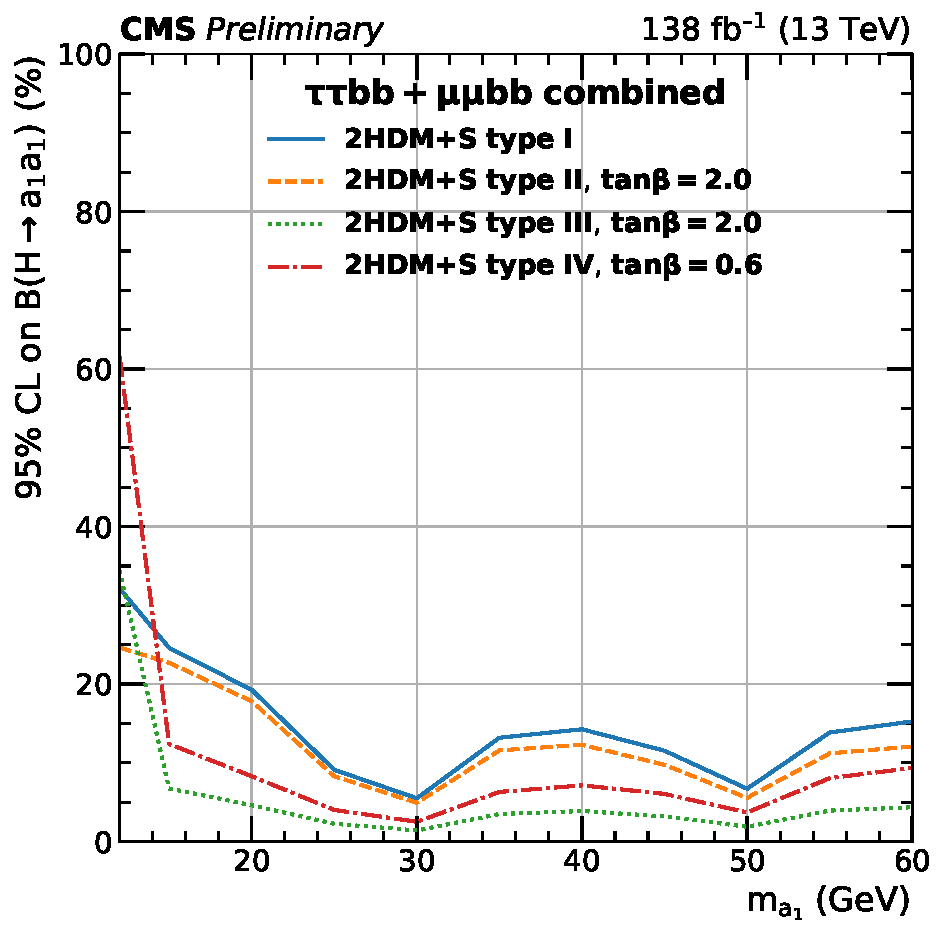
\includegraphics[width=0.6\textwidth]{figures/ch-10-results/HAA_comb_all_prelim.pdf}
    \end{center}
    \caption[Observed 95\% CL upper limits on the branching fraction of the 125 GeV Higgs boson to two pseudoscalars, $B(h\to aa)$, in percentages, as a function of the pseudoscalar mass $m_a$, in 2HDM+S type I (\textit{blue}), type II with $\tan\beta = 2.0$ (\textit{orange dashed}), type III with $\tan\beta = 2.0$ (\textit{dotted green}), and type IV with $\tan\beta = 0.6$ (\textit{red dashed}), for the combination of $bb\mu\mu$ and $bb\tau\tau$ channels using the full Run 2 integrated luminosity of 138 fb$^{-1}$.]{Observed 95\% CL upper limits on the branching fraction of the 125 GeV Higgs boson to two pseudoscalars, $B(h\to aa)$, in percentages, as a function of the pseudoscalar mass $m_a$, in 2HDM+S type I (\textit{blue}), type II with $\tan\beta = 2.0$ (\textit{orange dashed}), type III with $\tan\beta = 2.0$ (\textit{dotted green}), and type IV with $\tan\beta = 0.6$ (\textit{red dashed}), for the combination of $bb\mu\mu$ and $bb\tau\tau$ channels using the full Run 2 integrated luminosity of 138 fb$^{-1}$ \cite{CMS-AN-20-213}.}
      \label{fig:results_limits_combined}
  \end{figure}
  


\begin{figure}[h]
    \begin{center}
      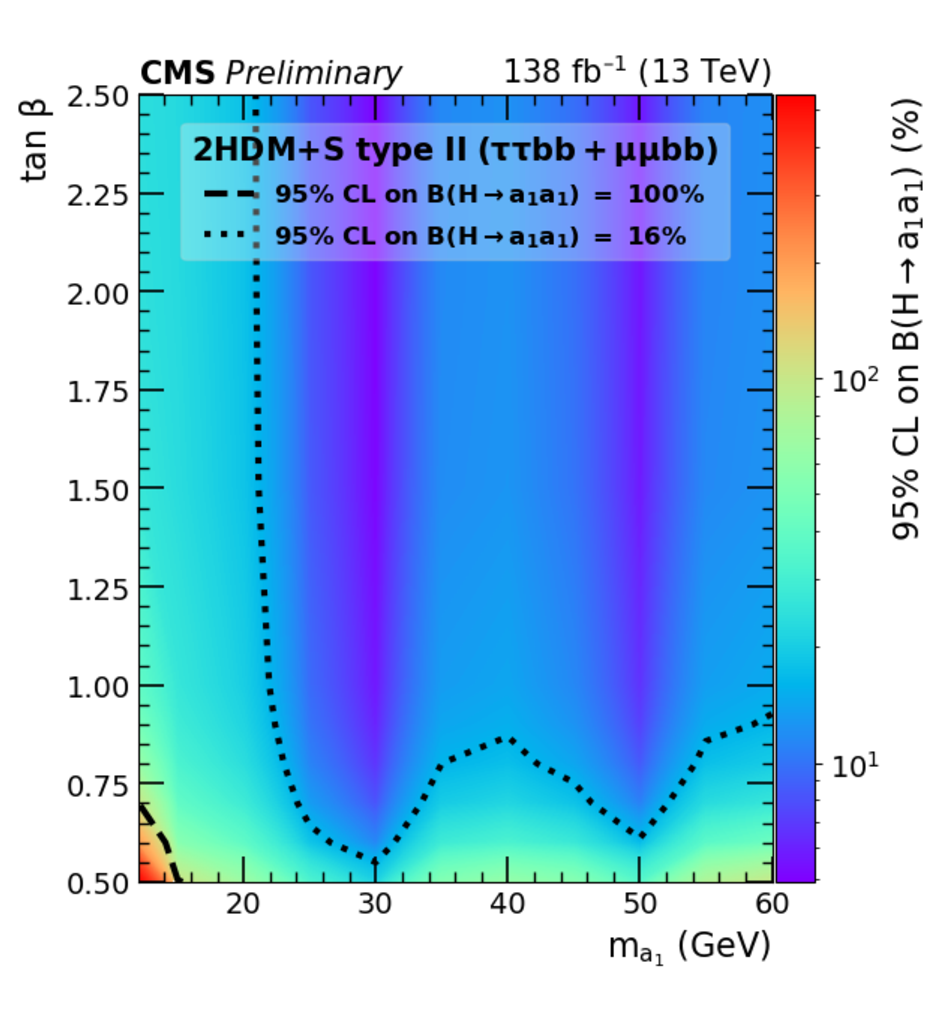
\includegraphics[width=0.32\textwidth]{figures/ch-10-results/HAA_comb_II_prelim.pdf}
      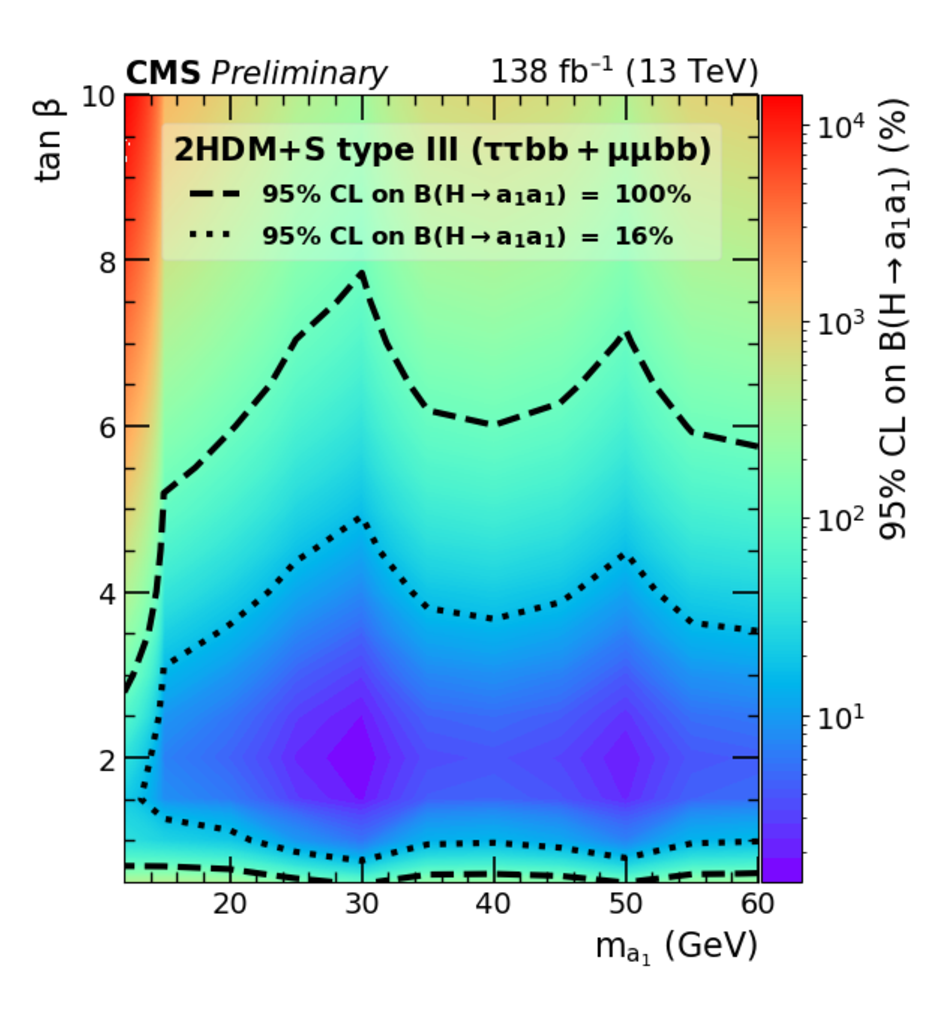
\includegraphics[width=0.32\textwidth]{figures/ch-10-results/HAA_comb_III_prelim.pdf}
      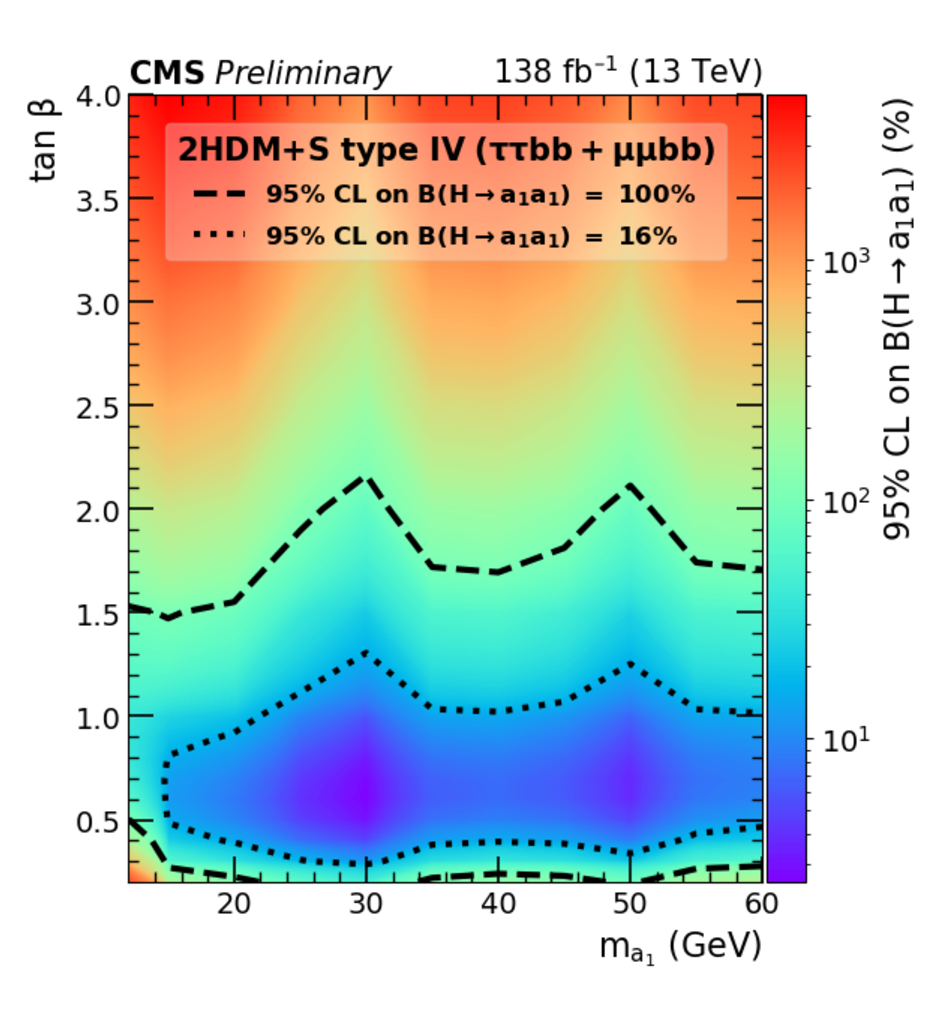
\includegraphics[width=0.32\textwidth]{figures/ch-10-results/HAA_comb_IV_prelim.pdf}
    \end{center}
    \caption[Observed 95\% CL upper limits on $\mathcal{B}(h\to aa)$ in \%, for the combination of $bb\mu\mu$ and $bb\tau\tau$ channels using the full Run 2 integrated luminosity of 138 fb$^{-1}$ for Type II (\textit{left}), Type III (\textit{middle}), and Type IV (\textit{right}) 2HDM+S in the $\tan\beta$ vs. $m_a$ phase space.]{Observed 95\% CL upper limits on $\mathcal{B}(h\to aa)$ in \%, for the combination of $bb\mu\mu$ and $bb\tau\tau$ channels using the full Run 2 integrated luminosity of 138 fb$^{-1}$ for Type II (\textit{left}), Type III (\textit{middle}), and Type IV (\textit{right}) 2HDM+S in the $\tan\beta$ vs. $m_a$ phase space. The contours (\textit{dashed black}) correspond to branching fractions of 100\% and 16\%, where 16\% is the combined upper limit on Higgs boson to undetected particle decays from previous Run-2 results. All points inside the contour are allowed within that upper limit. Linear extrapolation has been used between different points on the figures \cite{CMS-AN-20-213}.}
      \label{fig:results_limits_combined_2D}
  \end{figure}
  
The combined results from $h\rightarrow aa \rightarrow bb\ell\ell$ are compared with CMS results in other final states as a function of the pseudoscalar mass $m_a$: for 2HDM+S type I in Fig. \ref{fig:summary_plot_type_I}, type II with $\tan\beta = 2.0$ in Fig. \ref{fig:summary_plot_typeII_tan_beta_2p0}, and type III with $\tan\beta = 2.0$ in Fig. \ref{fig:summary_plot_typeIII_tan_beta_2p0}. In other scenarios, e.g. type III with $\tan\beta = 5.0$, more stringent limits are set by analyses in other final states, $\mu\mu\tau\tau$ in this case. Other summary plots for other model types and $\tan\beta$ values can be found at \cite{twiki_2HDM+S_summary-plots}.


\begin{figure}[h]
    \begin{center}
      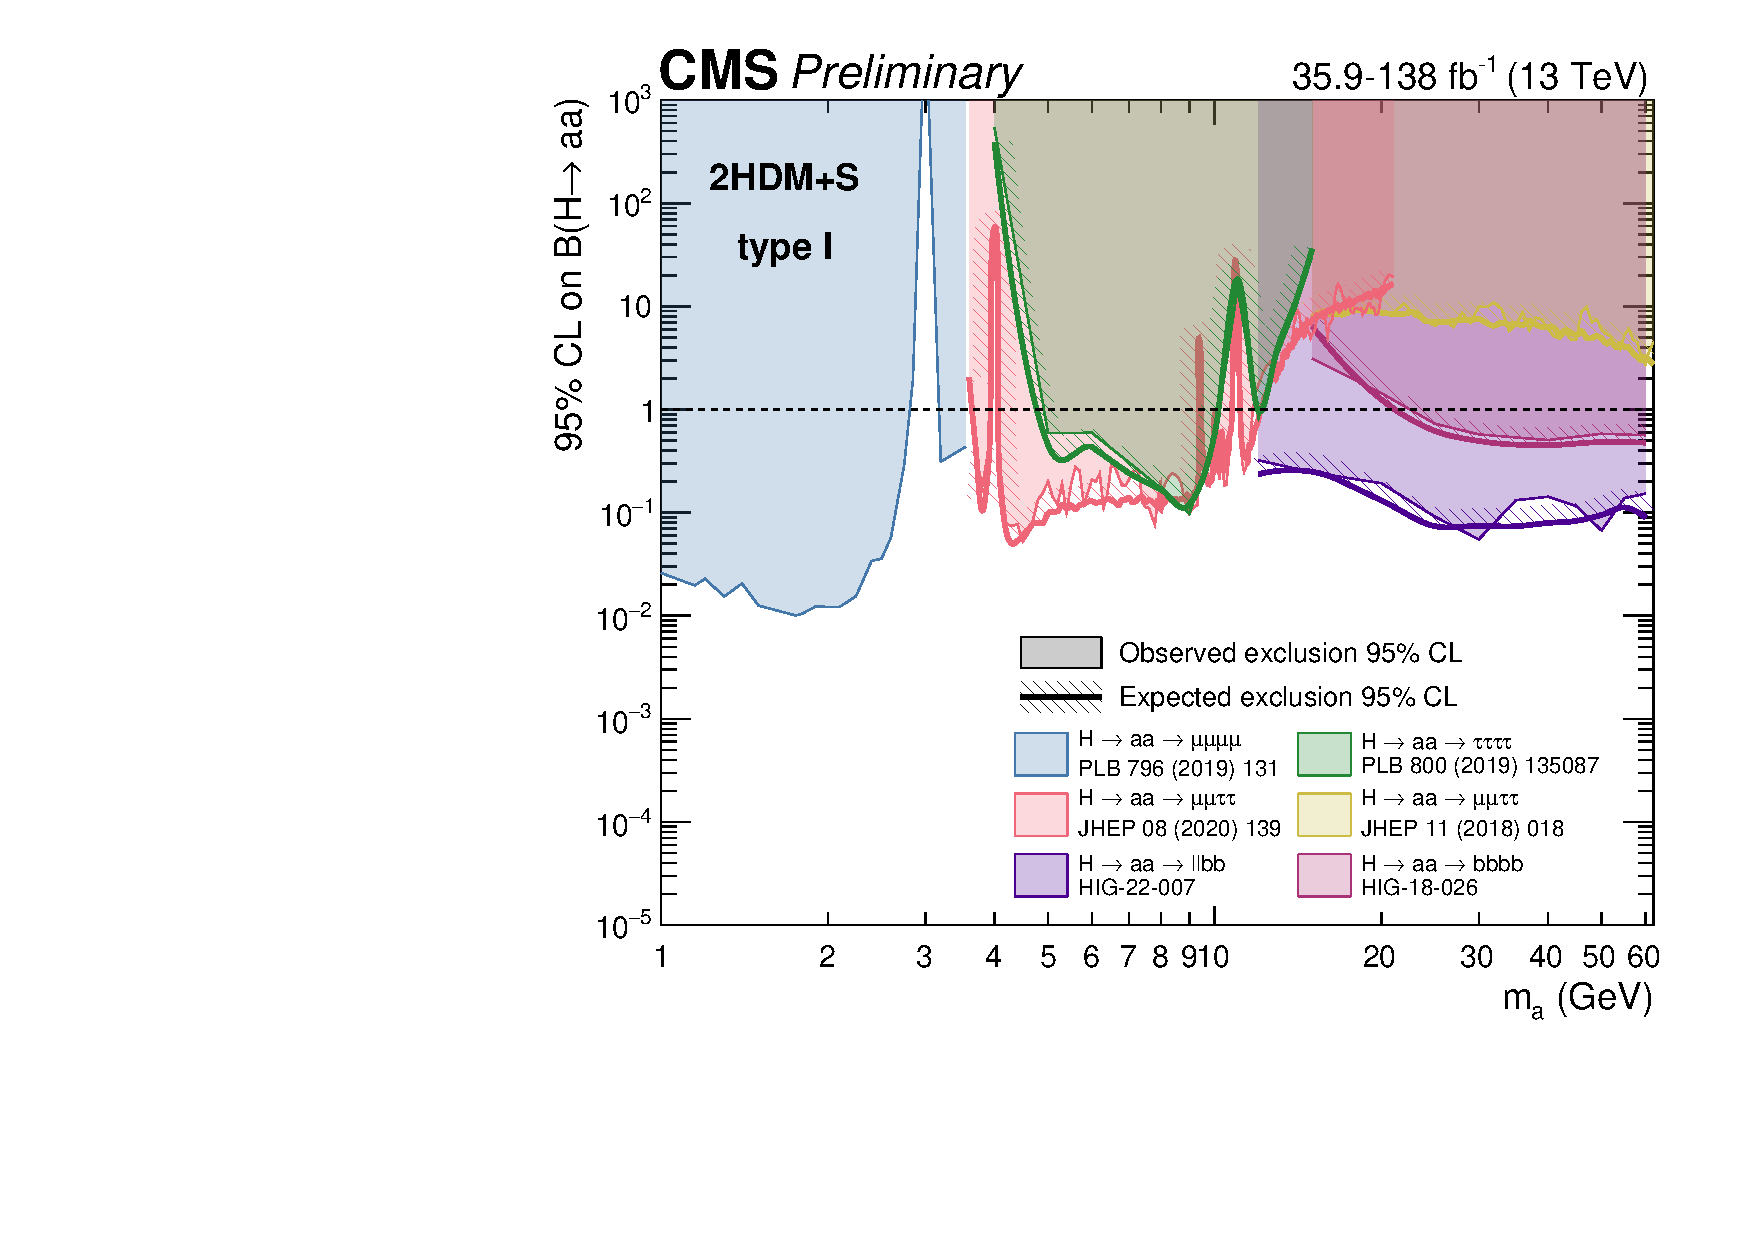
\includegraphics[width=0.6\textwidth]{figures/ch-10-results/summary_plot_full_run2_plot_BRaa_Type1.pdf}
    \end{center}
    \caption[Summary plot of current observed and expected 95\% CL limits on the branching ratio of the 125 GeV Higgs boson to two pseudoscalars, normalized to the Standard Model Higgs production cross-section, $\frac{\sigma(h)}{\sigma_{\text{SM}}} \times B(h \rightarrow aa)$, in the 2HDM+S type I scenario, obtained at CMS with data collected at 13 TeV.]{Summary plot of current 95\% limits on the branching ratio of the 125 GeV Higgs boson to two pseudoscalars, normalized to the Standard Model Higgs production cross-section, $\frac{\sigma(h)}{\sigma_{\text{SM}}} \times B(h \rightarrow aa)$ in the 2HDM+S type I scenario performed with data collected at 13 TeV \cite{twiki_2HDM+S_summary-plots}. Results from different final states studied at CMS are overlaid on this figure: $\mu\mu\mu\mu$ (\textit{blue}), $\tau\tau\tau\tau$ (\textit{green}), boosted $2\mu 2\tau$ (\textit{red}), resolved $2\mu 2\tau$ (\textit{yellow}), $bbbb$ (\textit{magenta}), and the combined result for $\ell\ell bb$ ($\ell = \mu, \tau$) (\textit{purple}).}
      \label{fig:summary_plot_type_I}
  \end{figure}
  \begin{figure}[h]
    \begin{center}
      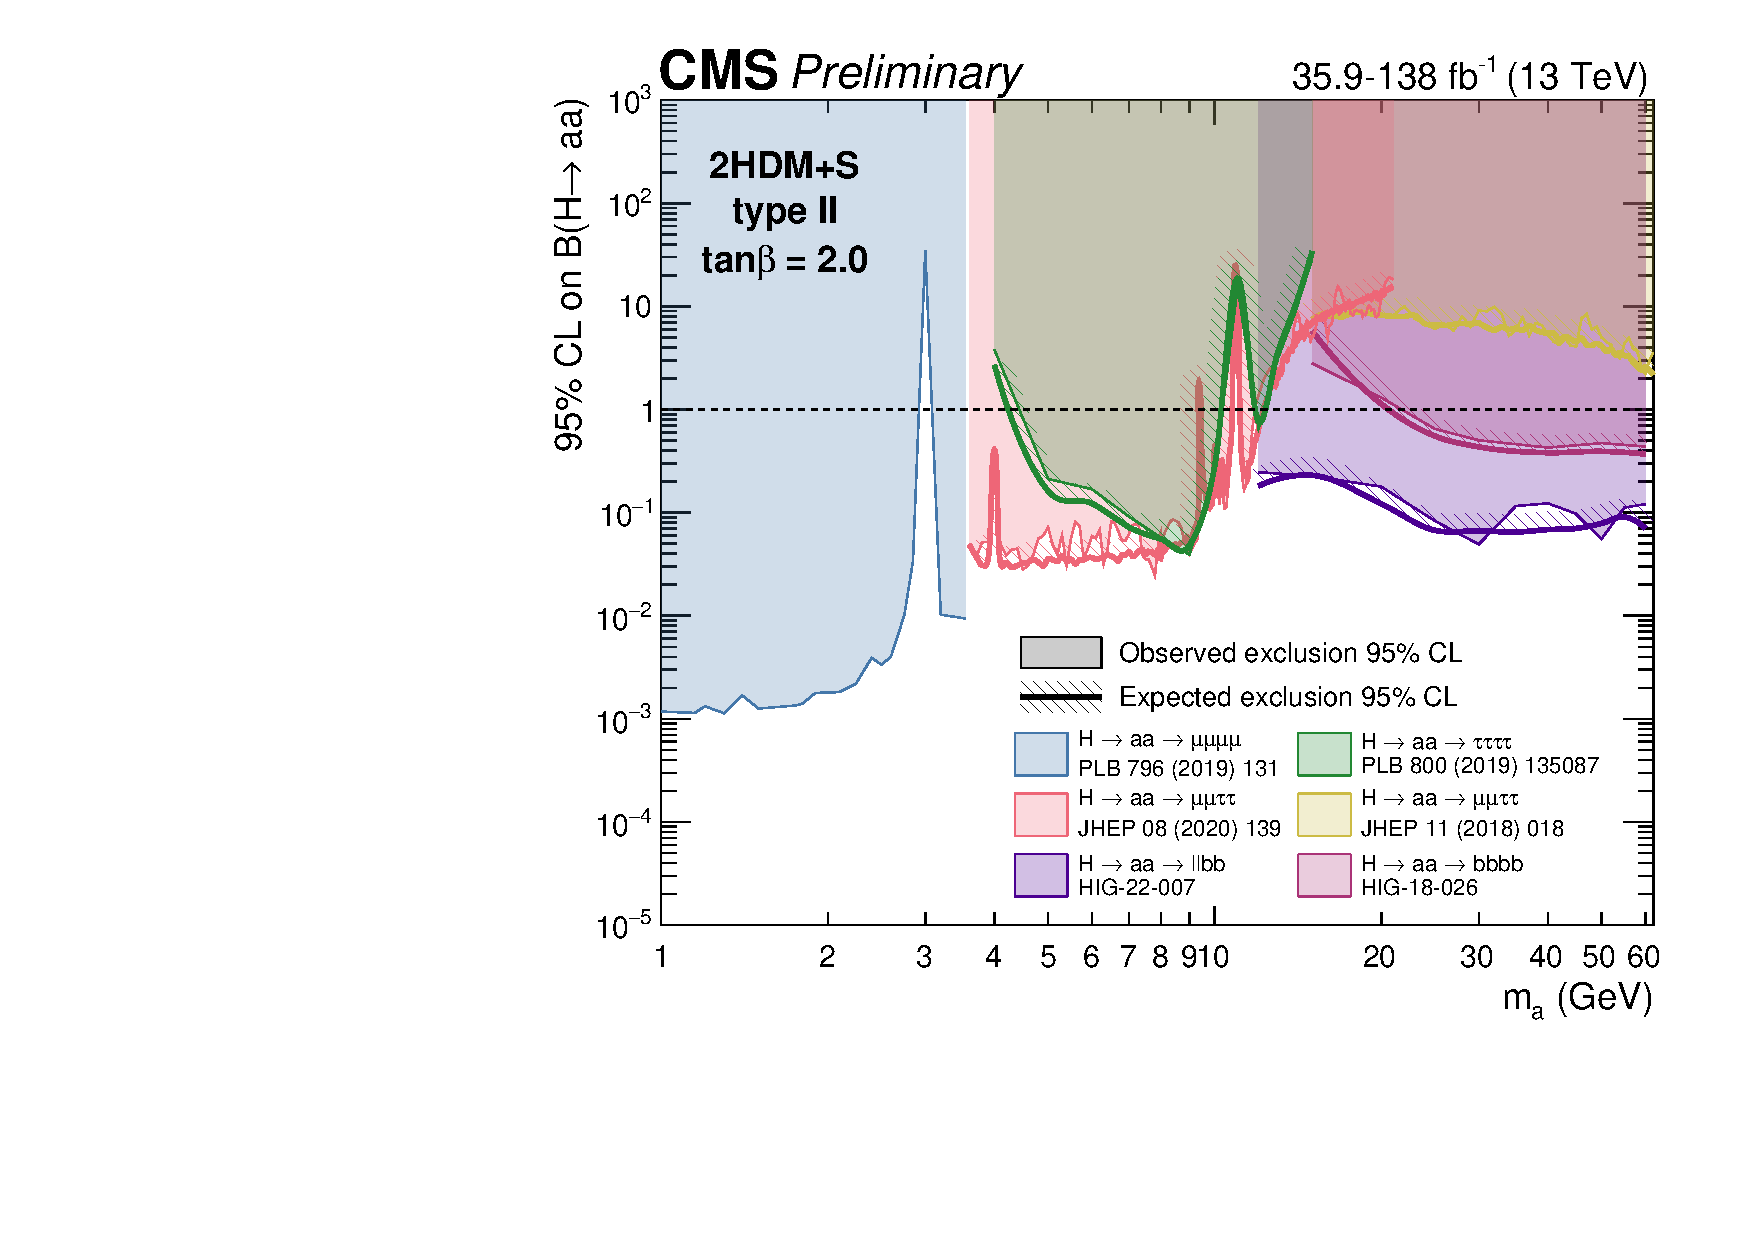
\includegraphics[width=0.6\textwidth]{figures/ch-10-results/summary_plot_full_run2_plot_BRaa_Type2_tanbeta2.pdf}
    \end{center}
    \caption[Summary plot of current observed and expected 95\% CL limits on the branching ratio of the 125 GeV Higgs boson to two pseudoscalars, normalized to the Standard Model Higgs production cross-section, $\frac{\sigma(h)}{\sigma_{\text{SM}}} \times B(h \rightarrow aa)$, in the 2HDM+S type II scenario with $\tan\beta = 2.0$, obtained at CMS with data collected at 13 TeV.]{Summary plot of current observed and expected 95\% CL limits on the branching ratio of the 125 GeV Higgs boson to two pseudoscalars, normalized to the Standard Model Higgs production cross-section, $\frac{\sigma(h)}{\sigma_{\text{SM}}} \times B(h \rightarrow aa)$, in the 2HDM+S type II scenario with $\tan\beta = 2.0$, obtained at CMS with data collected at 13 TeV \cite{twiki_2HDM+S_summary-plots}. Results from different final states studied at CMS are overlaid on this figure: $\mu\mu\mu\mu$ (\textit{blue}), $\tau\tau\tau\tau$ (\textit{green}), boosted $2\mu 2\tau$ (\textit{red}), resolved $2\mu 2\tau$ (\textit{yellow}), $bbbb$ (\textit{magenta}), and the combined result for $\ell\ell bb$ ($\ell = \mu, \tau$) (\textit{purple}).}
      \label{fig:summary_plot_typeII_tan_beta_2p0}
  \end{figure}
  \begin{figure}[h]
    \begin{center}
      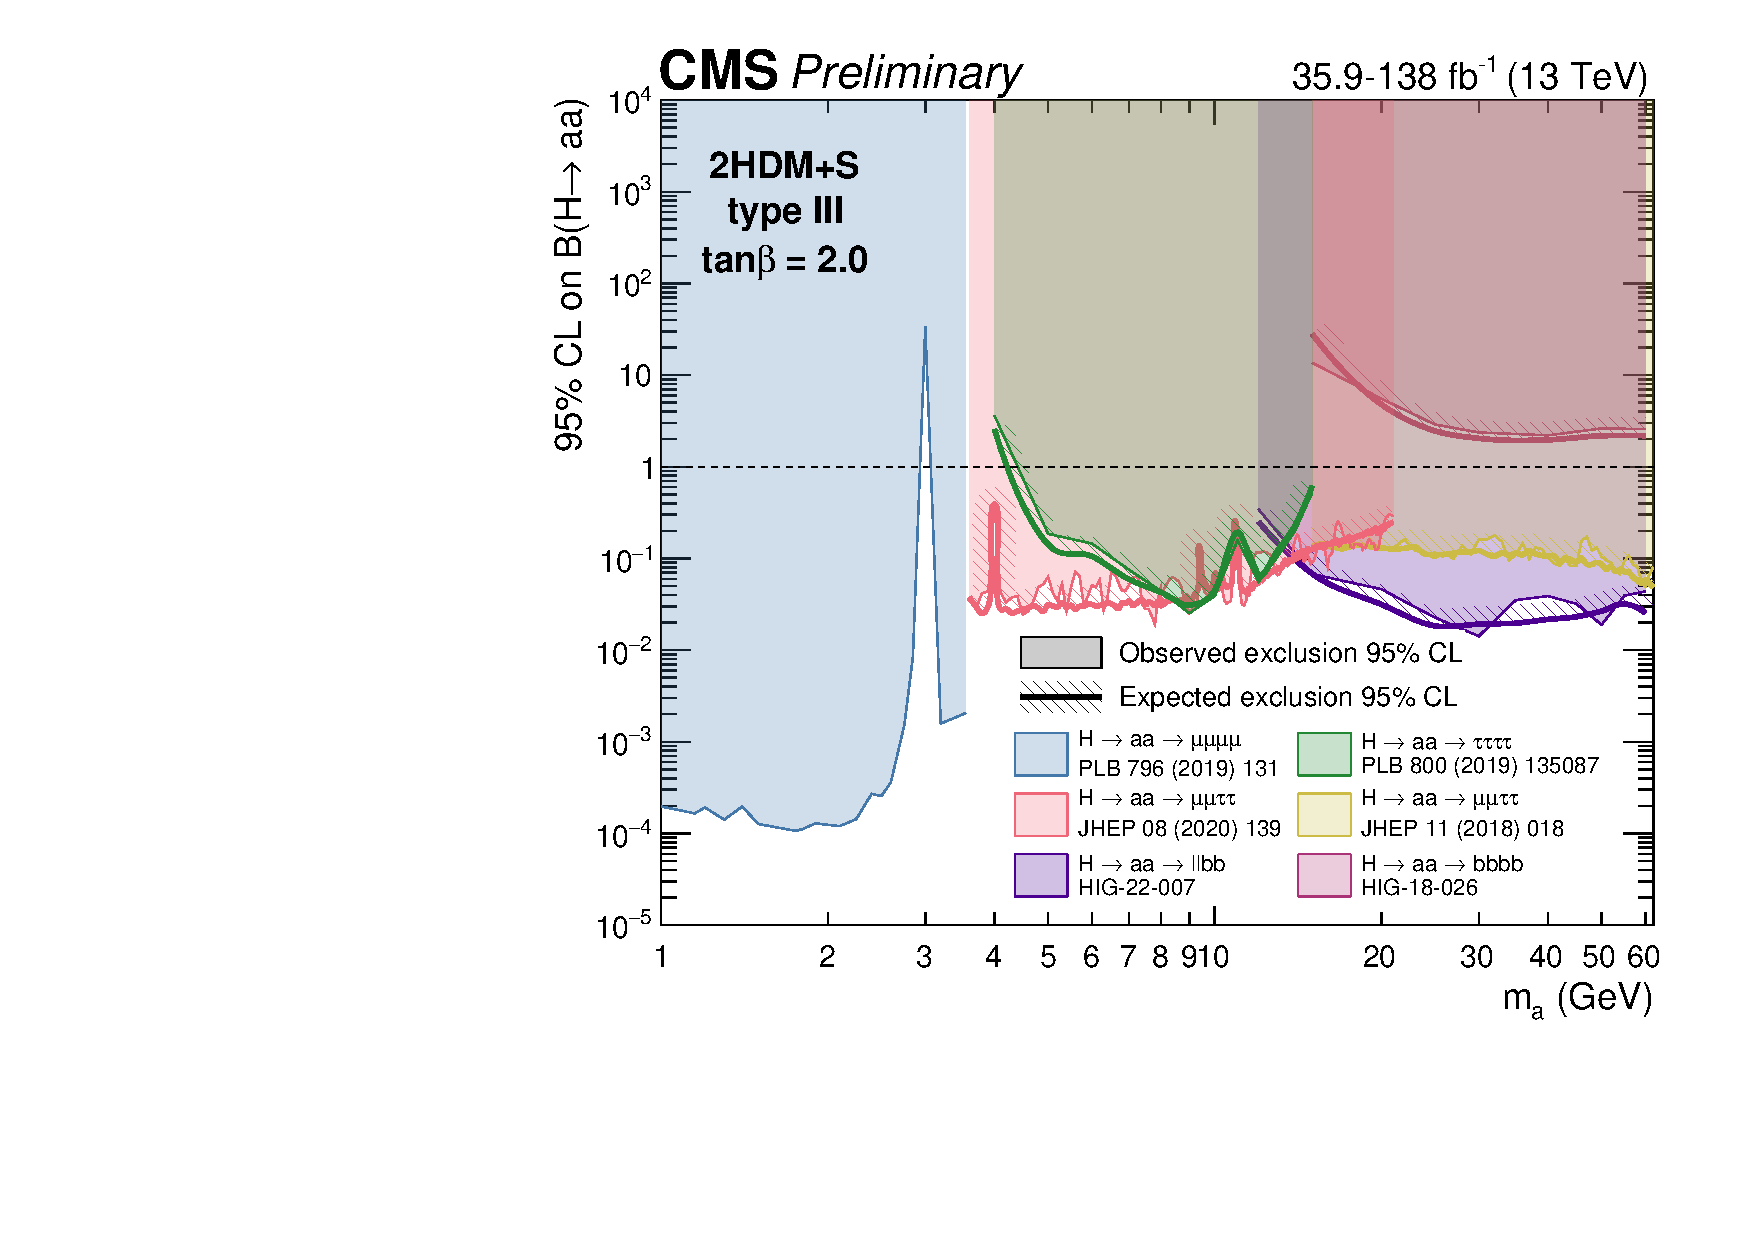
\includegraphics[width=0.6\textwidth]{figures/ch-10-results/summary_plot_full_run2_plot_BRaa_Type3_tanbeta2.pdf}
    \end{center}
    \caption[Summary plot of current observed and expected 95\% CL limits on the branching ratio of the 125 GeV Higgs boson to two pseudoscalars, normalized to the Standard Model Higgs production cross-section, $\frac{\sigma(h)}{\sigma_{\text{SM}}} \times B(h \rightarrow aa)$, in the 2HDM+S type III scenario with $\tan\beta = 2.0$, obtained at CMS with data collected at 13 TeV.]{Summary plot of current observed and expected 95\% CL limits on the branching ratio of the 125 GeV Higgs boson to two pseudoscalars, normalized to the Standard Model Higgs production cross section, $\frac{\sigma(h)}{\sigma_{\text{SM}}} \times B(h \rightarrow aa)$ in the 2HDM+S type-III scenario with $\tan\beta = 2.0$, obtained at CMS with data collected at 13 TeV \cite{twiki_2HDM+S_summary-plots}. Results from different final states studied at CMS are overlaid on this figure: $\mu\mu\mu\mu$ (\textit{blue}), $\tau\tau\tau\tau$ (\textit{green}), boosted $2\mu 2\tau$ (\textit{red}), resolved $2\mu 2\tau$ (\textit{yellow}), $bbbb$ (\textit{magenta}), and the combined result for $\ell\ell bb$ ($\ell = \mu, \tau$) (\textit{purple}).}
      \label{fig:summary_plot_typeIII_tan_beta_2p0}
  \end{figure}
  
